\documentclass[12pt]{article}
\usepackage[T1]{fontenc}

% Set page size and margins
% Replace `letterpaper' with`a4paper' for UK/EU standard size
\usepackage[a4paper,top=2cm,bottom=2cm,left=3cm,right=3cm,marginparwidth=1.75cm]{geometry}

% Useful packages
\usepackage{amsmath}
\usepackage{graphicx}
\usepackage{amsfonts}
\usepackage{fancyhdr}
\setlength{\headheight}{16pt}
\pagestyle{fancy}

\usepackage{hyperref}
\hypersetup{
    colorlinks,
    citecolor=black,
    filecolor=black,
    linkcolor=black,
    urlcolor=black
}

\usepackage{glossaries}
\usepackage{subfigure}
%\usepackage{dot2texi}

\makenoidxglossaries



\loadglsentries{lexique}


\usepackage[table,xcdraw, x11names, svgnames, rgb]{xcolor}
\usepackage[utf8]{inputenc}
\usepackage{eso-pic}
\usepackage{tikz}
\usetikzlibrary{shapes,arrows,positioning, snakes}
\usepackage{float}
\usepackage{textcomp}
\usepackage{soul}
\usepackage{listings}
\newcommand{\hilight}{\makebox[0pt][s]{\color{green!50}\rule[-3.6pt]{1.0\linewidth}{12pt}}}

\usepackage{tikz}
\usepackage{listofitems} % for \readlist to create arrays


\tikzstyle{mynode}=[thick, draw=blue, fill=blue!20,circle, minimum size=22]

\lstdefinestyle{xmlStyle}{
    language=XML,
    basicstyle=\ttfamily\small,
    numbers=left,
    numberstyle=\tiny\color{gray},
    stepnumber=1,
    numbersep=10pt,
    backgroundcolor=\color{white},
    showspaces=false,
    showstringspaces=false,
    showtabs=false,
    frame=single,
    tabsize=2,
    captionpos=b,
    breaklines=true,
    breakatwhitespace=false,
    title=\lstname,
    keywordstyle=\color{blue},
    commentstyle=\color{gray},
    stringstyle=\color{red},
}

\definecolor{mygray}{rgb}{0.5,0.5,0.5}
\lstdefinestyle{command}{
  backgroundcolor=\color{white},
  basicstyle=\ttfamily\color{black},
  keywordstyle=\color{blue},
  commentstyle=\color{mygray},
  stringstyle=\color{red},
  showstringspaces=false,
  upquote=true,
  morekeywords={sudo, ls, cd, mv, cp, rm, mkdir, chmod, chown, grep, find},
  captionpos=b,
  frame=single,
  numbers=left,
  numberstyle=\tiny\color{mygray},
  breaklines=true,
  breakatwhitespace=true,
  tabsize=2,
  keepspaces=true,
  caption={Linux Command},
  label=command,
}
\lstdefinestyle{bashstyle}{
  backgroundcolor=\color{white},
  basicstyle=\ttfamily\color{black},
  keywordstyle=\color{blue},
  commentstyle=\color{mygray},
  stringstyle=\color{red},
  showstringspaces=false,
  upquote=true,
  morekeywords={sudo, ls, cd, mv, cp, rm, mkdir, chmod, chown, grep, find},
  captionpos=b,
  frame=single,
  numbers=left,
  numberstyle=\tiny\color{mygray},
  breaklines=true,
  breakatwhitespace=true,
  tabsize=2,
  keepspaces=true,
  caption={Script bash},
  label=command,
}

\lstdefinestyle{cstyle}{
    language=C,
    basicstyle=\ttfamily,
    keywordstyle=\color{blue},
    commentstyle=\color{green!40!black},
    stringstyle=\color{red},
    identifierstyle=\color{black},
    captionpos=b,
    numbers=left,
    numberstyle=\tiny\color{gray},
    frame=single,
    breaklines=true,
    showstringspaces=false,
    tabsize=4,
    morekeywords={int, char, void, if, else, while, for, return, typedef, struct, include},
    columns=flexible
}

\lstdefinestyle{makefilestyle}{
    language=make,
    basicstyle=\ttfamily,
    keywordstyle=\color{blue},
    commentstyle=\color{green!40!black},
    captionpos=b,
    stringstyle=\color{red},
    identifierstyle=\color{black},
    numbers=left,
    numberstyle=\tiny\color{gray},
    frame=single,
    breaklines=true,
    showstringspaces=false,
    tabsize=4,
    morekeywords={ifeq, endif, else, ifdef, ifndef, define, endef, export, unexport, obj},
    columns=flexible
}
\lstdefinestyle{config}{
    language=make,
    basicstyle=\ttfamily,
    keywordstyle=\color{blue},
    commentstyle=\color{green!40!black},
    captionpos=b,
    stringstyle=\color{red},
    identifierstyle=\color{black},
    numbers=left,
    numberstyle=\tiny\color{gray},
    frame=single,
    breaklines=true,
    showstringspaces=false,
    tabsize=4,
    morekeywords={ifeq, endif, else, ifdef, ifndef, define, endef, export, unexport, obj},
    columns=flexible
}

% YANL style for listings (mainly ROS2 params files)
\lstdefinestyle{yaml}{
    morekeywords={true,false,null,y,n},
    sensitive=false,
    morecomment=[l]{\#},
    morestring=[b]',
    morestring=[b]",
    basicstyle=\ttfamily,
    keywordstyle=\color{blue},
    commentstyle=\color{green!40!black},
    captionpos=b,
    stringstyle=\color{red},
    identifierstyle=\color{black},
    numbers=left,
    numberstyle=\tiny\color{gray},
    frame=single,
    breaklines=true,
    showstringspaces=false,
    tabsize=4,
    columns=flexible
}


\bibliographystyle{plain} % We choose the "plain" reference style

\renewcommand{\epsilon}{\varepsilon} 
\renewcommand{\phi}{\varphi} 
\title{Final Year Project Report\vspace{10pt}\\
**************************************************\\
Multi Agent Scene Exploration and Mapping \\
for Continuous Digital Twin Creation\vspace{10pt}\\
**************************************************}
\author{BELPOIS Vincent \\ Under the supervision of Dr. Ivan \textsc{Mutis}}

\begin{document}
\emergencystretch 3em
\date{2024}
\maketitle
\thispagestyle{empty}

\vspace{10mm}

\begin{center}

\includegraphics[width = 6cm]{Images/logo_ensma.png}
\end{center}
\vspace{2cm}
\begin{center}
    
\includegraphics[width = 8cm]{Images/IIT_Logo_stack_186_blk.png}
\end{center}
\vspace{1cm}
\begin{center}
    
\includegraphics[width = 6cm]{Images/logo_iconsense_bloack_text.png}
\end{center}
\newpage
\thispagestyle{empty}
\mbox{}




\AddToShipoutPictureBG{%
\put(15,7){
\includegraphics[scale = 0.02]{Images/logo_ensma.png}}
\put(480,10){
\includegraphics[width = 100pt]{Images/IIT_Logo_stack_186_blk.png}}
\put(400,14.9){
\includegraphics[width = 75pt]{Images/logo_iconsense_bloack_text.png}}
}



\newpage
\section*{Acknowledgments}

    Acknowledgments.
    
\newpage
\thispagestyle{empty}
\mbox{}
\newpage
\thispagestyle{empty}
{\small \tableofcontents}

\newpage
\thispagestyle{empty}
\mbox{}
\newpage

\section{Introduction}

    The internship took place at the Illinois Institute Technology (IIT) in Chicago, the largest city of the state of the state of Illinois and the Midwest of the United States.

    \subsection{Presentation of IIT}

    The Illinois Institute of Technology (IIT) is a private research university in Chicago, Illinois. It was established in 1940 by the merger of the Armour Institute and Lewis Institute. The university has programs in computer science, architectural and building sciences, mechanical engineering, information technologies, bioenginnering and biomedical engineering, civil engineering, aerospace, aeronautical and astraunotical engineering, chemical engineering, electrical and electronics engineering, and more.


    \subsection{Presentation of the lab}

    I was part of the iConSenSe Lab, a lab that focuses on advanced computing, informatics, sensing, and semantics technologies for civil and construction engineering. The lab currently focuses mainly on how virtual and mixed reality can enhance the construction industry, through VR based training. As construction Environments can be dangerous, a VR based training for safety rules and procedures can be very useful, as dangerous scenarios can be simulated safely.
    But the lab also explores technologies that could improve the construction quality and speed. Specifically, robotics could improve repetitive tasks on construction sites like picking up trash, or moving materials.


    \subsection{Context and goal of the project}   
    
    The problem we wish to tackle during this internship is the creation of point clouds for quality assurance purposes and progress tracking during construction. This is currently done with stationary 3D scanners that sit on tripods that need to be moved multiple times to cover the whole site. As this scanning process takes a long time to perform, they can not be performed regularly, and they require an operator to be present.
   
    We propose a system where multiple robotics agents can explore the construction site autonomously, performing the task daily or while construction is happening. Each agent carries a LIDAR sensor and fuses the data with the other agents in real time. This would allow a continuous digital twin to be made from the captured point cloud data and compared to the building information modeling (BIM) data. This could allow for fine grain inventory tracking of equipment, raw materials in the form of bags, pallets boxes, or piles of aggregate.
   
    We demonstrate a solution to this problem by showcasing exploration of a construction site like environment using a wheeled robot and a quadruped robot, with the intention of adding a quadcopter to perform mapping in areas that are inaccessible to the other platforms. This solution currently does not provide collaboration between the different agents but aims to build towards this objective. 

\newpage

\section[Setting up the physical agents]{Setting up the physical agents}
\label{section:big title}%label to reference section

        The goal of this project was to have three different kinds of platforms, to showcase the versatility of the algorithms considered. We chose to focus on a wheeled platform, a quadruped robot, and a quadcopter. Each platform could show its strengths and weakness in certain situations, while the algorithms would remain largely similar between the platforms. This section explains how the various agents were set up in terms of the hardware modifications, the sensors being fitted, and the software setup.

        %Three platforms were used in this project: a six-wheeled platform, a quadcopter, and a quadruped platform. Each platform was chosen for its specific characteristics, with the goal of having a multi-agent system that could explore and map a scene. The wheeled platform was chosen for its stability and ability to carry heavy loads. The quadcopter was chosen for its ability to fly and provide a bird's-eye view of the scene. The quadruped platform was chosen for its ability to climb stairs and navigate bumpy terrain.

    \subsection{Wheeled platform setup}

        The wheeled platform was chosen for its stability on flat terrain and with other projects in mind, its ability to carry heavy loads. The intent was to have a robotic arm mounted for other projects. Some previous work had already been done on the platform, but the person was apparently unsuccessful. These earlier attempts had left the platform in a partially modified state, requiring a comprehensive reassessment and redesign of both the mechanical and electrical systems. Despite these setbacks, the robust chassis of the six-wheeled platform still presented an excellent foundation for our project, offering the potential for further development.

        \subsubsection{Mechanical modifications}
        As it arrived, the six-wheeled platform only consisted of a stainless steel chassis, six DC motors, and wheels, as can be seen in Figure \ref{fig:wheeled_latform}. The platform required several mechanical modifications to accommodate the necessary components for autonomous operation. Specifically, it needed a mount for a LIDAR sensor and an embedded computer on its top surface (see Figure \ref{fig:motor_driver_mount}). The inside was reserved for the motors, battery, and power circuitry. Additionally, a mounting solution for the motor drivers inside the chassis was essential (see Figure \ref{fig:motor_driver_mount}), as the previous version didn't secure them in place and had several drivers stop functioning. These modifications were designed and implemented to ensure proper integration of all components while maintaining the structural integrity of the platform, the integration of the LIDAR and the embedded computer can be seen in Figure \ref{fig:full_cad_model}.
        
        \begin{figure}[H]
            \centering
            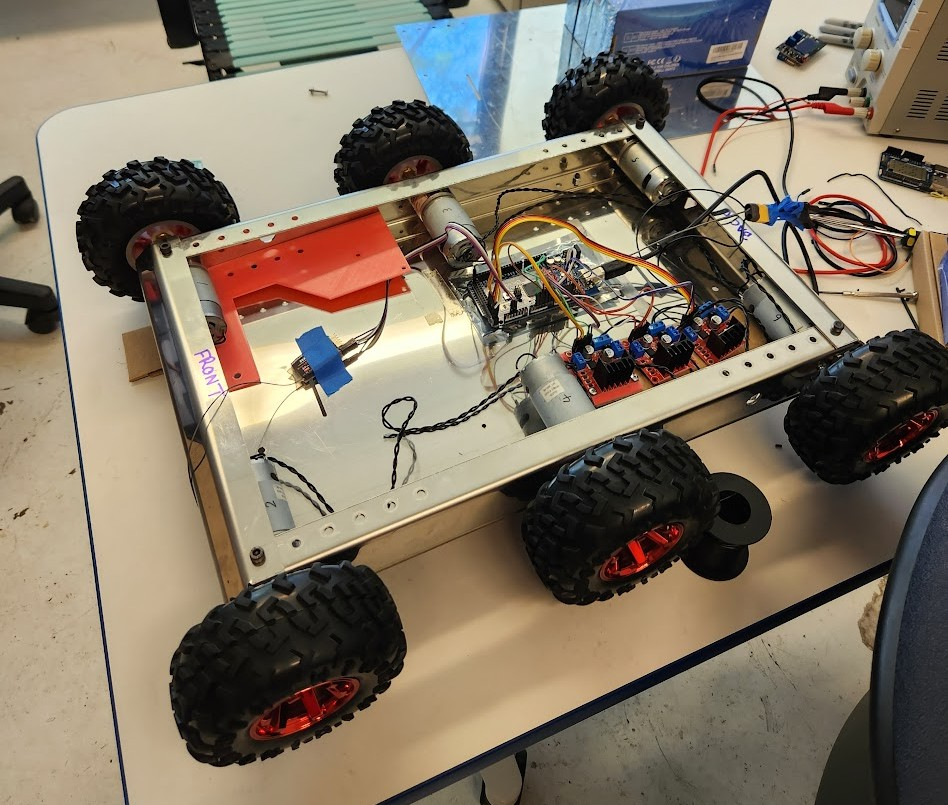
\includegraphics[width=0.5\textwidth]{Images/wheeled_platform_empty.jpg}
            \caption{Chassis of the six-wheeled platform during the installation of the motor drivers}
            \label{fig:wheeled_latform}
        \end{figure}


        \begin{figure}[H]
            \centering
            %MOTOR DRIVER MOUNT CAD
            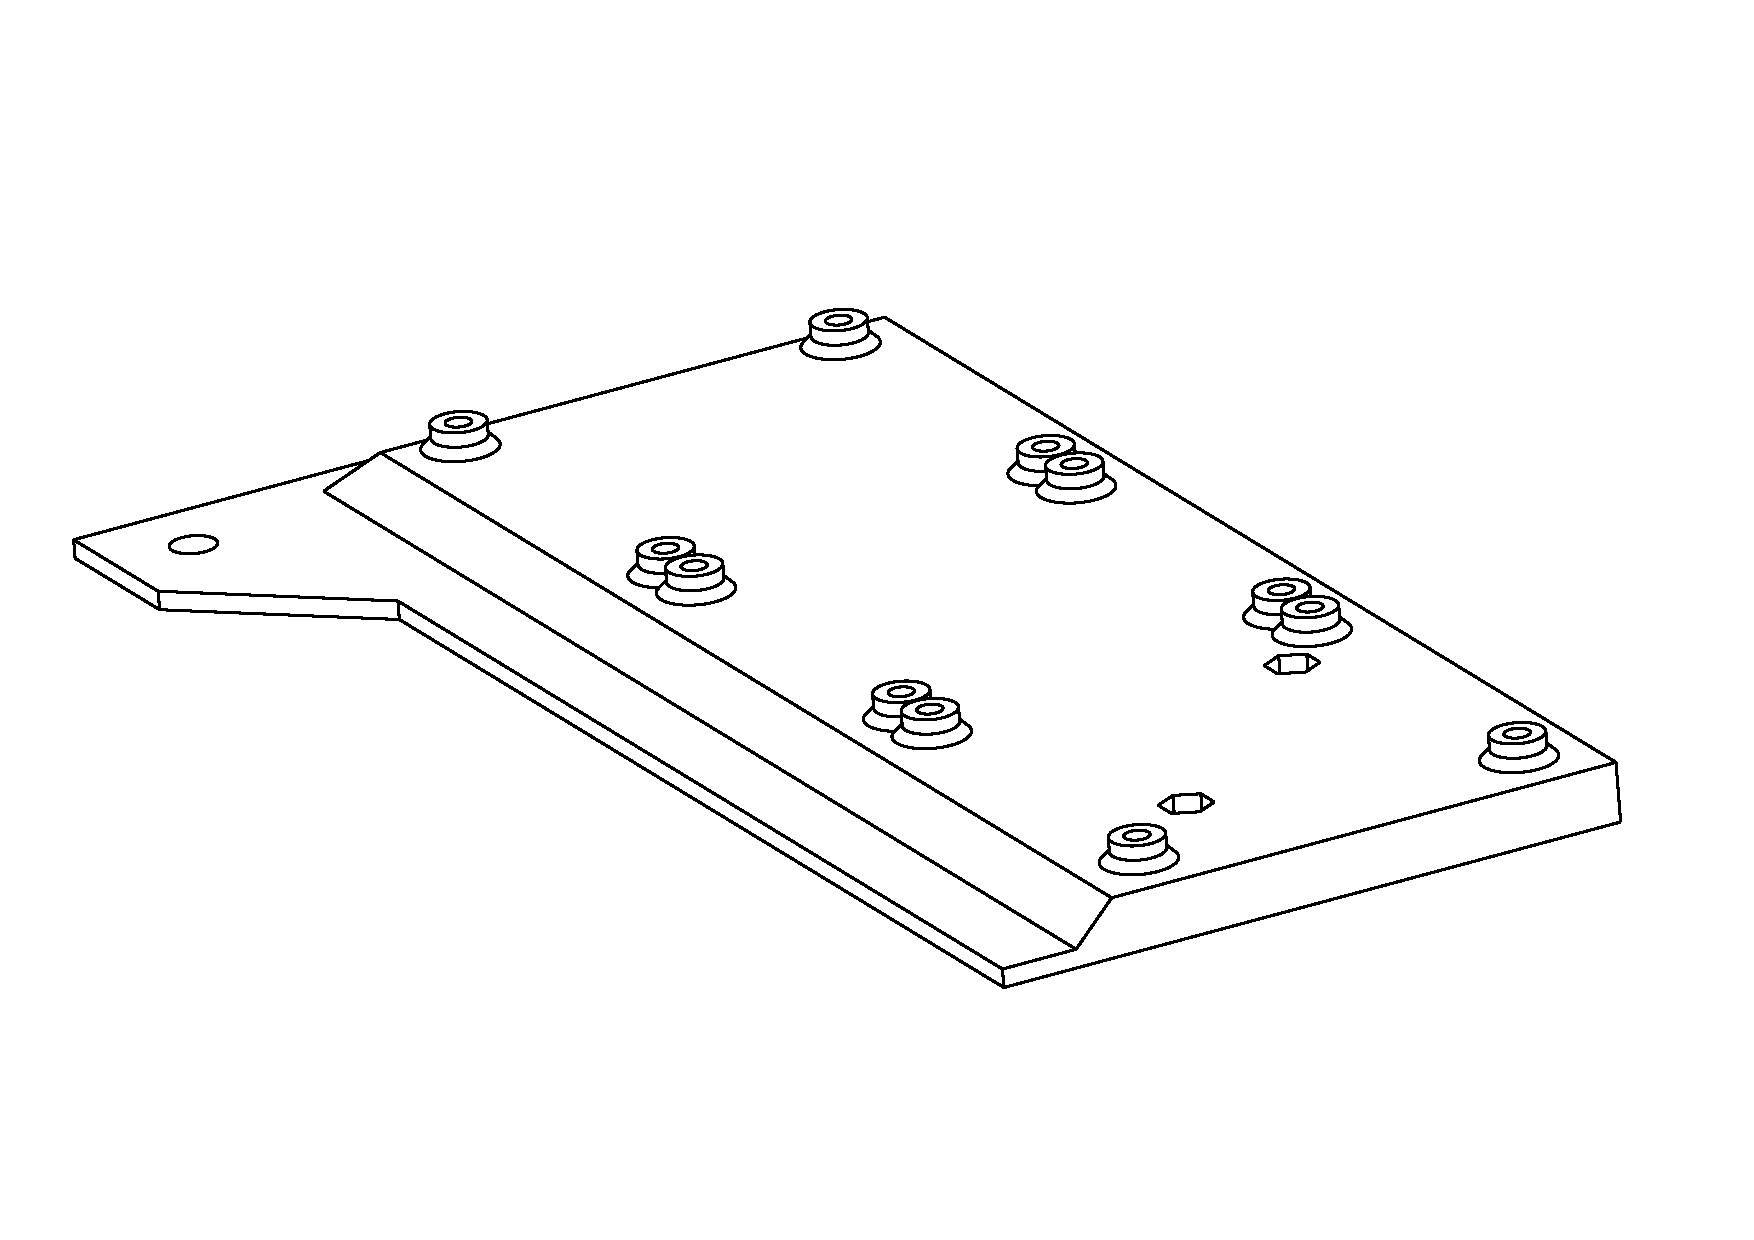
\includegraphics[width=0.3\textwidth]{Images/Motor_driver_holder.pdf}
            \caption{Drawing of CAD model of the motor driver mounting solution}
            \label{fig:motor_driver_mount}
        \end{figure}
        
        To further accelerate development of the construction of the robots, a 3D printer was purchased and set up by myself. We chose the Bambu Lab P1P 3D printer for its large enclosed build volume, which would allow us to print engineering materials such as ABS, Nylon, or carbon fiber filed materials. It required a nozzle to be changed to hardened steel to be able to handle fiber filled filaments, which I performed and tested by printing protection cages for the LIDARs. The printer was set up in the lab and was used to print the parts needed for the mechanical modifications of the platforms. It was also used to print parts for other projects in the lab, such as storage for VR headsets, and all kinds of brackets.

        \begin{figure}[H]
            \centering
            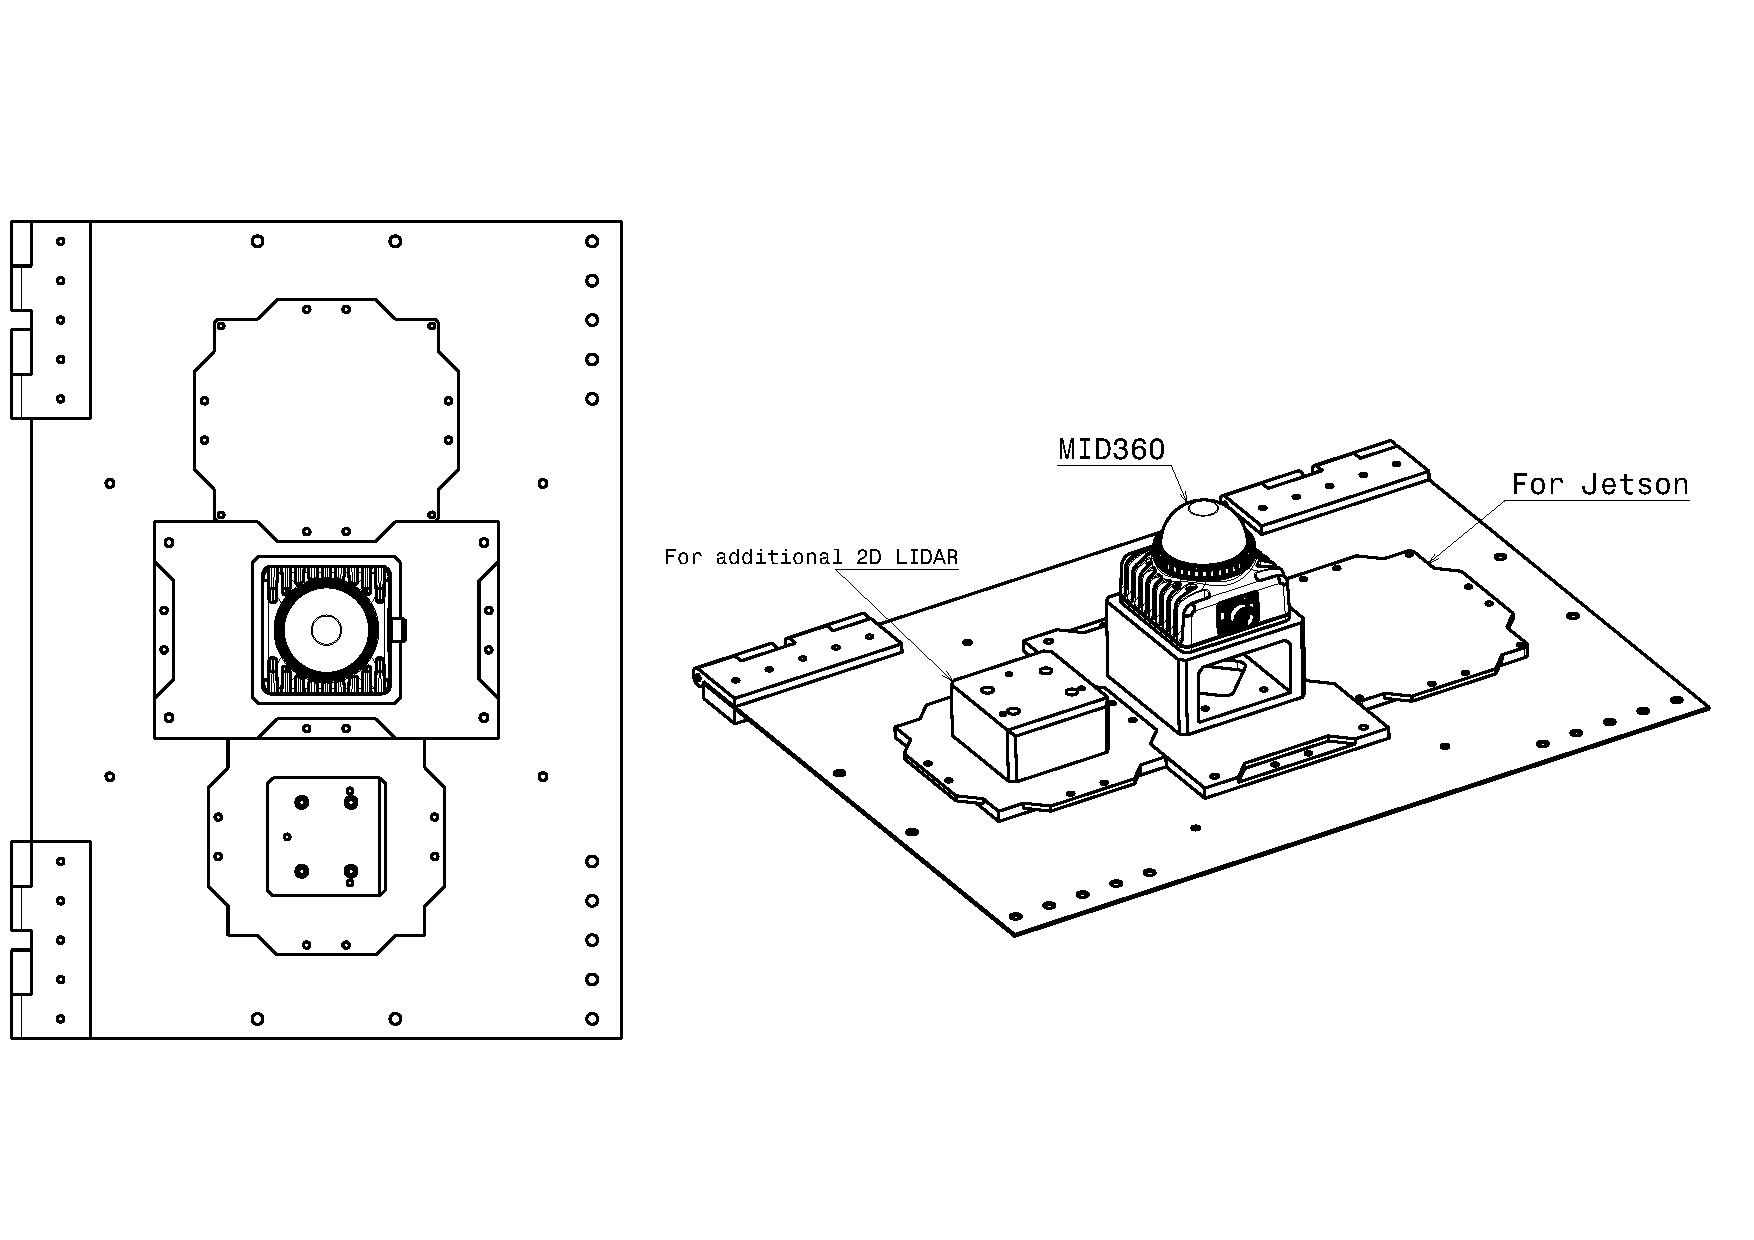
\includegraphics[width=0.8\textwidth]{Images/RoverV1.pdf}
            \caption{Drawing of CAD model of the modified six-wheeled platform's top}
            \label{fig:full_cad_model}
        \end{figure}

        \subsubsection{Electronics architecture}
            The essential electronic components needed to get the platform running were mainly DC motor drivers to drive the motors, a LIDAR sensor and an embedded computer.
            
            Difficulties were encountered when trying to use the drivers someone else tried beforehand as they were under powered : at stall, the motors required around 5 amps of current, as measured with a bench top power supply, and the drivers I was trying to use were only capable of delivering 2 amps per channel or a total of 4 amps when combining outputs. The drivers in question were the based on the LN298N which were in terms replaced by the 7A dual motor drivers from DFRobot. A physical comparison can be seen in Figure \ref{fig:drivers_comparison}.
        
            
            \begin{figure}[h]
                \centering
                %INSERT (a) (b) PICTURE OF BOTH DRIVERS
                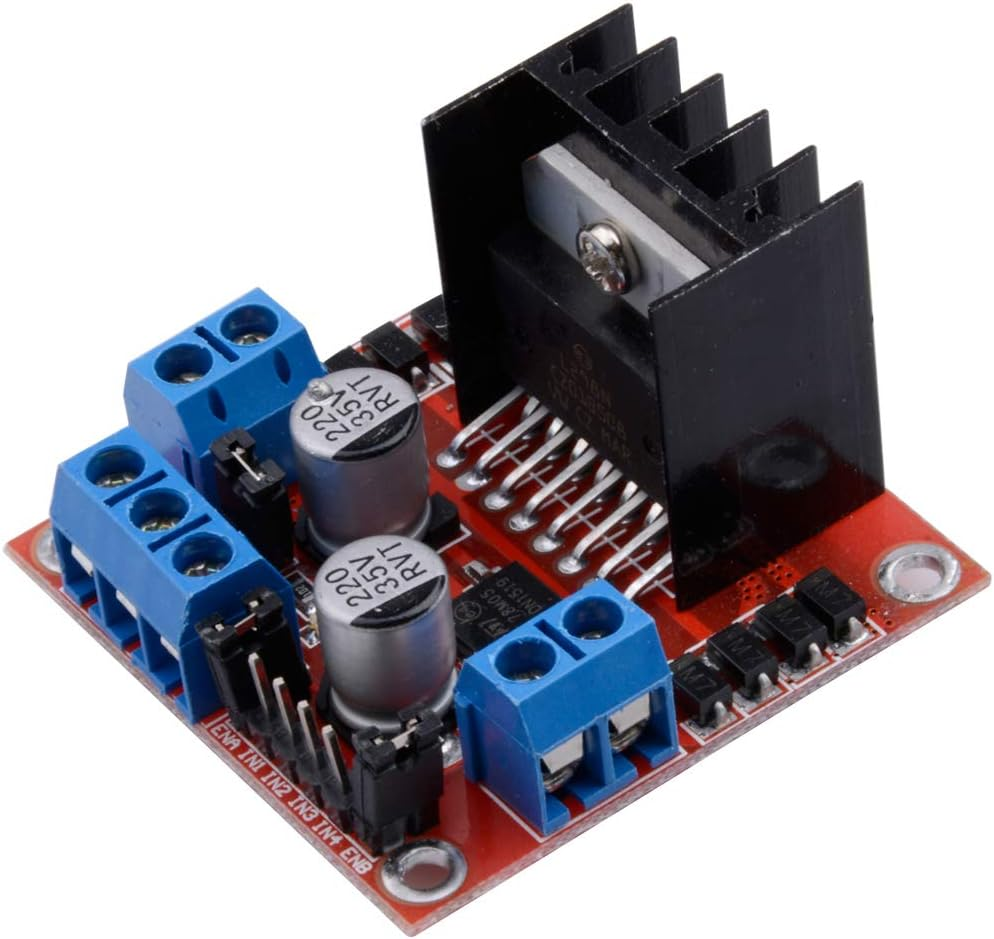
\includegraphics[width=0.3\textwidth]{Images/olddrivers.jpg}
                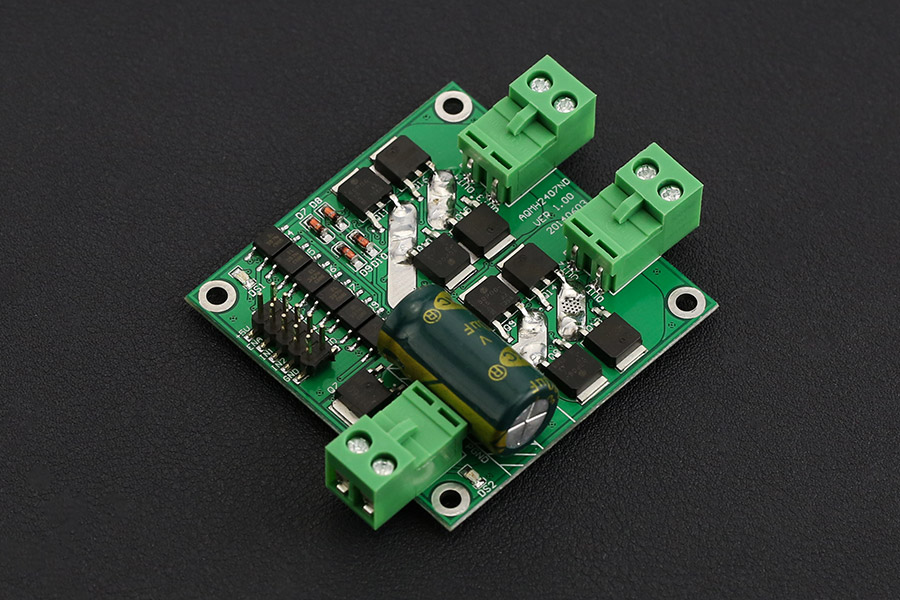
\includegraphics[width=0.4\textwidth]{Images/newdrivers.jpg}
                \caption{L298N (left) and DFRobot 7A dual DC Motor Driver (right)}
                \label{fig:drivers_comparison}
            \end{figure}

            The three motor drivers were connected to a microcontroller through custom made cables, as the cables previously used were undersized for the current of the motors. The connection can be seen in Figure \ref{fig:driver_to_pico}, as well as the connection from the microcontroller to the radio receiver.
            I chose to use a Raspberry Pi Pico microcontroller for its many outputs, totaling 22 general purpose input outputs (GPIO). Each driver required 6 control signals or 3 per motor: two signals are used to control the direction of the motor according to Table \ref{tab:motor_control}, while the third signal's duty cycle determines the speed.

            A radio control (RC) receiver was also connected to interrupt capable GPIOs of the microcontroller to be able to control the platform manually. We use interrupts for those signals as to measure the pulse duration accurately and thus infer the control signal sent via radio. Three channels of the RC receiver were used to control the speed, the direction and the mode of the platform. The mode refers to whether or not the platform is in manual control or in autonomous mode and is connected to channel 5 of the radio which has a two-way switch.

            Finally, the Pico is connected to an Nvidia Jetson Orin single board computer (SBC) via USB. This connection is used both to reprogram the Pico, and to send speed and direction commands to each motor via a serial communication. 

            We chose a Jetson Orin as it has a powerful GPU, which is not the case for many other SBCs like Raspberry Pis, and is designed for robotics applications in mind. Even though the algorithms we are using don't make use of the GPU and the CUDA cores, other applications like machine vision, or certain machine learning based terrain traversability methods could benefit from it \cite{beycimen2023comprehensive}. Small form factor computers featuring x86 based processors were also considered and would have offered more CPU performance, but powering them and interfacing with them would have been more difficult as they are not designed for robotics.
            
            To summarize the different connections of all the components, Figure \ref{fig:overall_electical_system} shows the electrical connections of these components on the modified six-wheeled platform, excluding power distribution and regulation.


            \begin{table}[h!]
                \centering
                \begin{tabular}{|c|c|c|c|}
                \hline
                IN1 & IN2 & ENA/ENB & Motor1/2 Behavior \\ \hline
                0   & 0   & x       & Stop (brake)      \\ \hline
                1   & 1   & x       & Vacant            \\ \hline
                1   & 0   & 1       & Forward 100\%     \\ \hline
                0   & 1   & 1       & Reverse 100\%     \\ \hline
                1   & 0   & PWM     & Forward at PWM speed \\ \hline
                0   & 1   & PWM     & Reverse at PWM speed \\ \hline
                \end{tabular}
                \caption{Motor control signal table, where 1 is a high signal and 0 is a low signal}
                \label{tab:motor_control}
            \end{table}

            \begin{figure}[H]
                \centering
                %OVERALL ELECTRICAL SYSTEM (excluding power)
                
                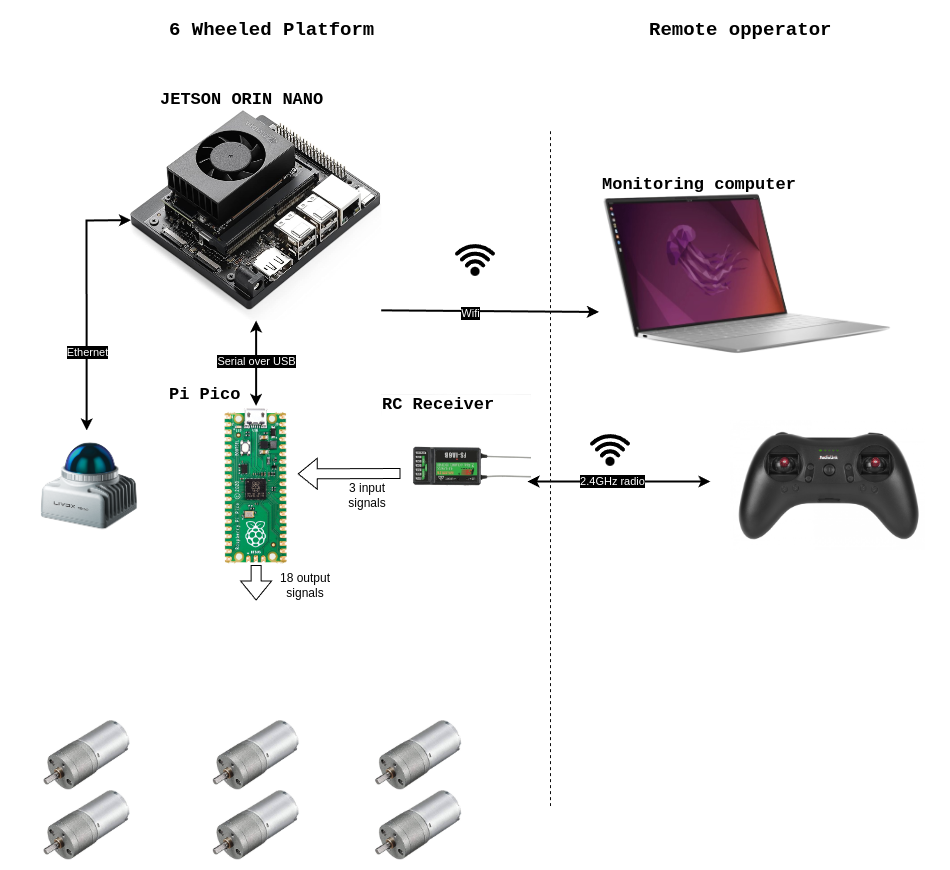
\includegraphics[width=0.8\textwidth]{Images/PFE-Page-2.drawio.png}
                \caption{Overall electrical system, excluding power distribution and regulation}
                \label{fig:overall_electical_system}
            \end{figure}


            
            
            \begin{figure}[h]
                \centering
                \mbox{}\clap{
                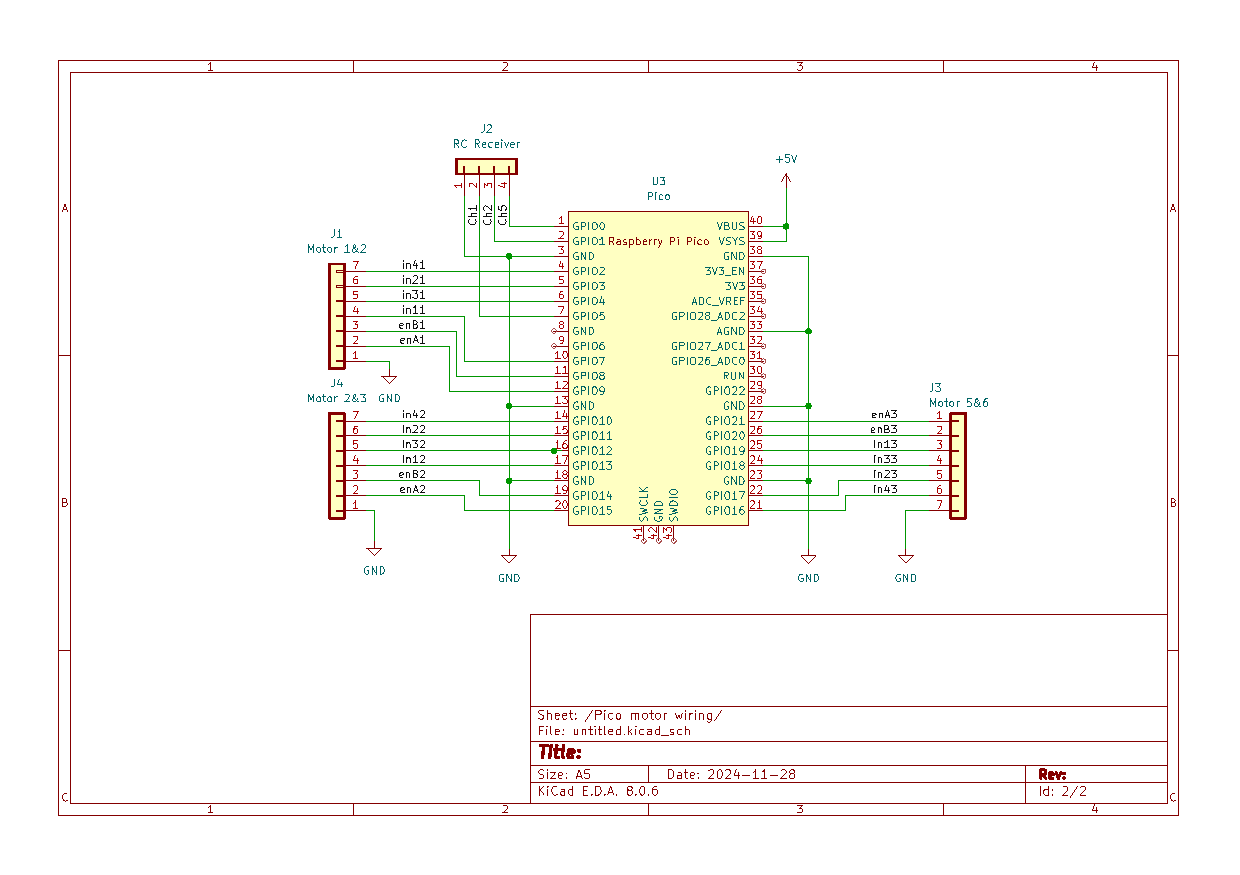
\includegraphics[width=0.9\paperwidth]{Images/PicoWiring.pdf}
                }
                \caption{Wiring of the Raspberry Pi Pico to the motor drivers and to the RC receiver}
                \label{fig:driver_to_pico}
            \end{figure}

        
        
        \subsubsection{Software architecture}

        %How the software on the jetson communicates with the microcontroller and how it communicates with the LIDAR. The choice of the odometry algorithm will be explain in another section (master, comparison of multiple algo)

        The robot operating system (ROS) was chosen as the software framework for the platform running on the Jetson Orin embedded computer. Specifically, ROS2 Humble Hawksbill was selected due to its extensive package availability and compatibility with the Jetson Orin's hardware. Indeed, I was made aware of the struggles of another researcher running a ROS based robot on an Nvidia Jetson Nano and how Ubuntu, and ROS version mismatch may bring problems. 
        
        This version of ROS2 provides a robust and flexible framework for developing and integrating various components of the platform, including sensor processing, navigation, and control. For real-time critical tasks such as motor control and RC radio interrupts, the Raspberry Pi Pico microcontroller was utilized, leveraging its ability to handle low-level, time-sensitive operations. The microcontroller's firmware was developed from the ground up by myself, guaranteeing reliable execution of motor control and interrupt handling tasks. By combining the strengths of ROS2 on the Jetson Orin with the real-time capabilities of the Raspberry Pi Pico, the platform achieves a robust and efficient software architecture that enables seamless integration of autonomous navigation, sensor processing, and manual control. This software architecture is illustrated in Figure \ref{fig:SW_architecture}.

        \begin{figure}[H]
            \centering
            %Software stack, from jetpack to ros2 to the nodes to the microcontroller
            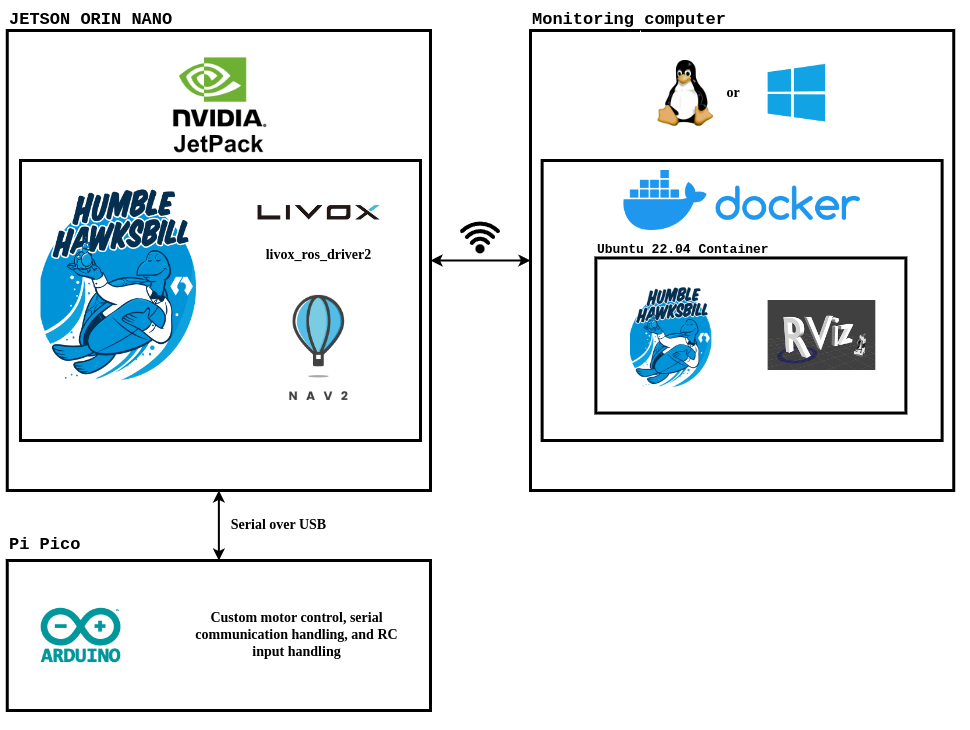
\includegraphics[width=0.8\textwidth]{Images/Software architecture rover.drawio.png}
            \caption{Software architecture}
            \label{fig:SW_architecture}
        \end{figure}


        \subsubsection{ROS 2 setup}
        
        As the distribution of Linux that we use on the Jetson is derived from Ubuntu 22.04, ROS2 can be installed using the Debian packages provided by the ROS2 foundation. The installation process is straightforward \cite{ros2_installation} and is well documented on the ROS2 website. ROS2 packages are often built for multiple architecture include x86, and ARM32. The Jetson Orin being an ARM64 architecture, the packages are directly compatible with it. 

        The specific distribution of Linux that we decided to install is Jetson Linux 36.4, also called Jetpack 6.1. This distribution is based on Ubuntu 22.04 and the Linux kernel 5.15. The main advantage of using this Linux distribution over any other is the included Nvidia drivers, and the included libraries like CUDA\cite{cuda}, TensorRT \cite{tensorrt}, cuDNN\cite{cudnn}, VPI and many others. These libraries are essential for the use of the Jetson Orin as a computer vision and machine learning platform. The inference capabilities were not explored during this internship, but the embedded computer could be used for future sim to real \cite{peng2018sim} experiments. 

        In ROS2 a controller was created for handling the differential control of the robot. This packaged followed the interfaces provided by ros2\_control, allowing the seamless control of the robot both in simulation and in real life. The package I created for this is called \texttt{skid\_drive\_controller} and is largely inspired by the differential controller provided by the ros2\_control package.
        
        \noindent
        \begin{minipage}{0.45\textwidth}
            As can be seen in Figure \ref{fig:ros_control_diagram}, taken from the ros2\_control documentation, controllers request interfaces from the controller manager. The controller manager has previously received information from sensors, actuators, or systems that want to provide command or state interface. In our case, a modified version of the \texttt{diff\_drive\_arduino} takes care of providing one control interface and one state interface per wheel. Our \texttt{skid\_drive\_controller} then takes care of receiving data like wheel velocity from the state interfaces, and sends commands to the control interfaces. In the case of the Gazebo simulation, the simulator provides the state and command interfaces to the resource manager, which make our controller unaware of the fact that it is running in simulation.
        \end{minipage}%
        \hspace{3pt}
        \begin{minipage}{0.5\textwidth}
            \begin{figure}[H]
            \centering
                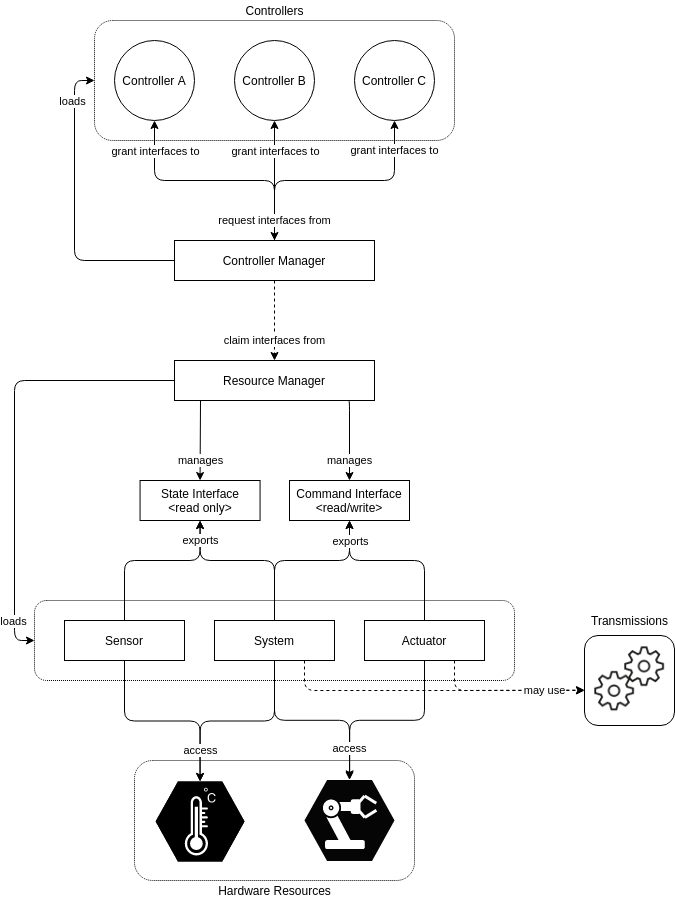
\includegraphics[width=0.99\textwidth]{Images/ros2_control.png}
                \caption{ROS2\_control architecture}
                \label{fig:ros_control_diagram}
                \end{figure}
        \end{minipage}

        % What nodes did I create, explain the setup with nav2 working.
        % TODO : Write a small paragraph in order to explain how ROS2 is setup and what external packages we need

        \subsubsection{Issues encountered}
            
        %Explain the state reached (nav2 navigation kinda working) and why the other platform was created

        The 6-wheeled rover, with its stainless steel frame and weak DC motors lacking encoders, was not the most suitable platform for the task of autonomous navigation. The lack of encoders on the motors made odometry calculations based on the LIDAR and inertial measurement unit unreliable. An attempt was made to do closed-loop control with the aforementioned odometry, but the noise and the lack of per-wheel odometry made it impossible to have a stable and reliable control.

        After encountering too many issues with the existing platform, we decided to create a new platform using closed-loop stepper motors, also called servos. Their closed-loop control and high torque at low speed would make them ideal for slow movements, thereby making the task of autonomous navigation feasible. A comparison of both platforms can be seen in Figure \ref{fig:rover_comparison}.

        \begin{figure}[H]
            \centering 
            \subfigure[Version 1 of the rover]{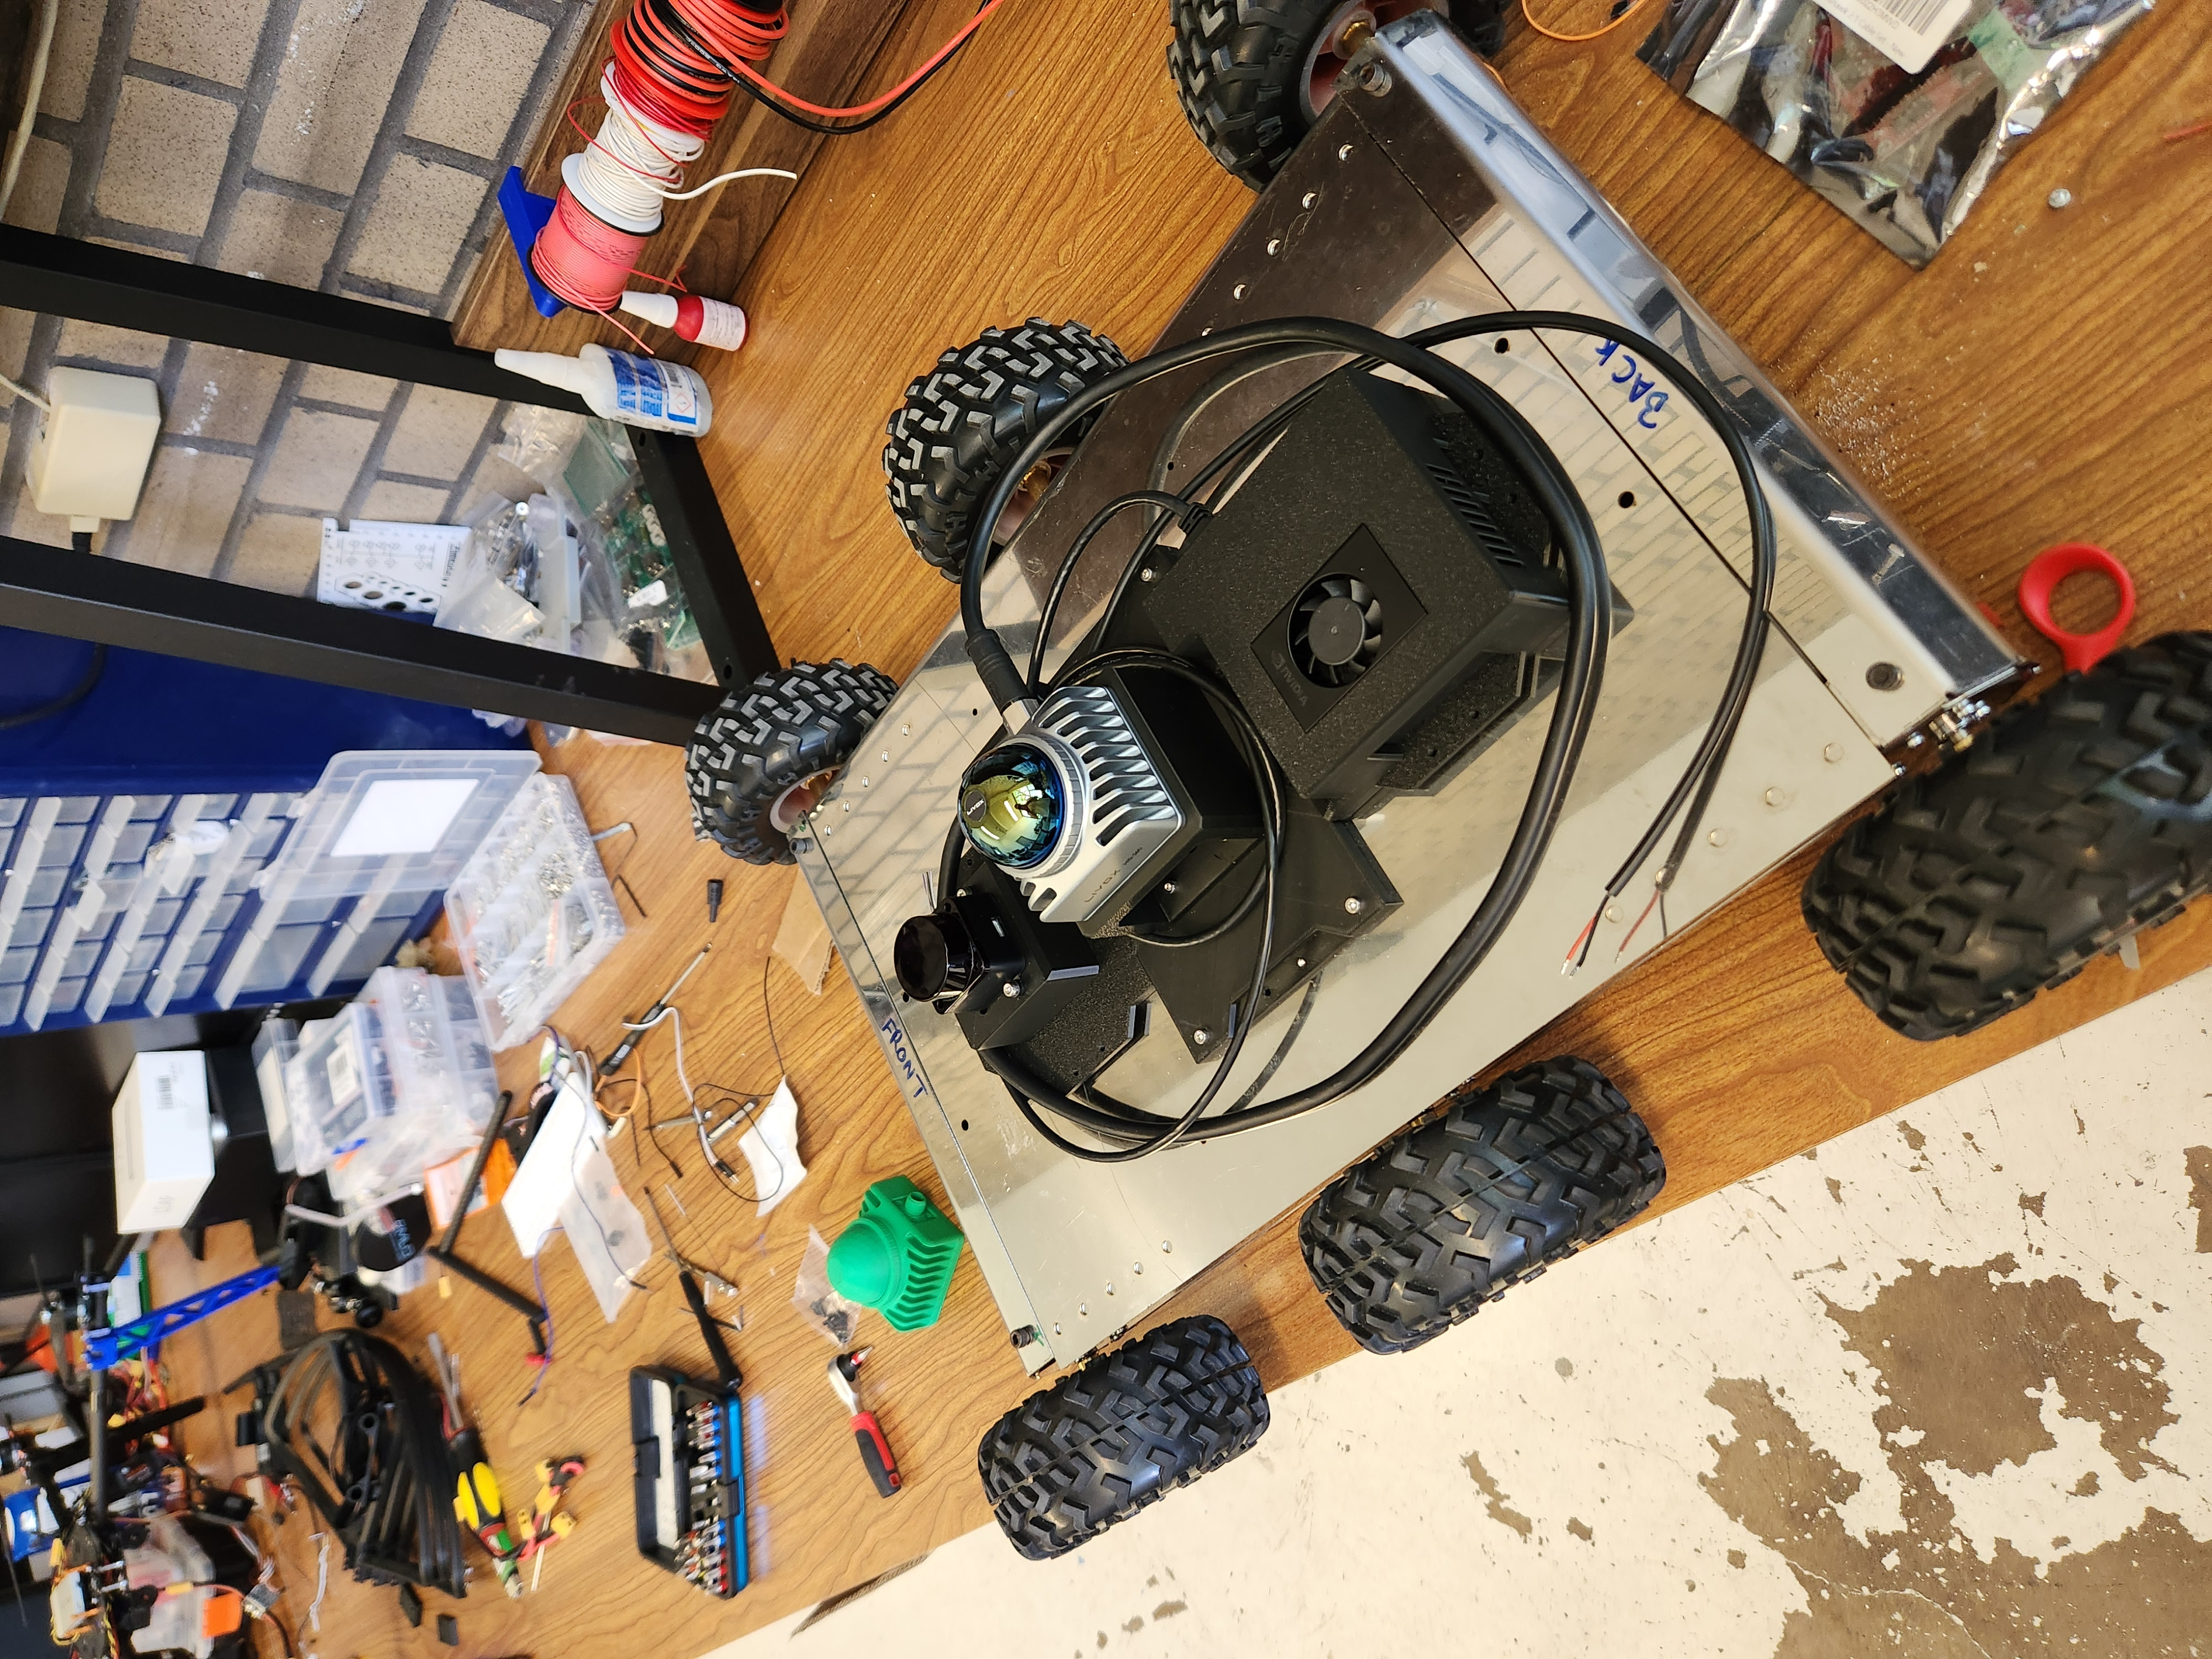
\includegraphics[width=0.4\textwidth, angle=270]{Images/roverv1closed.jpg}}
            \subfigure[Version 2 of the rover]{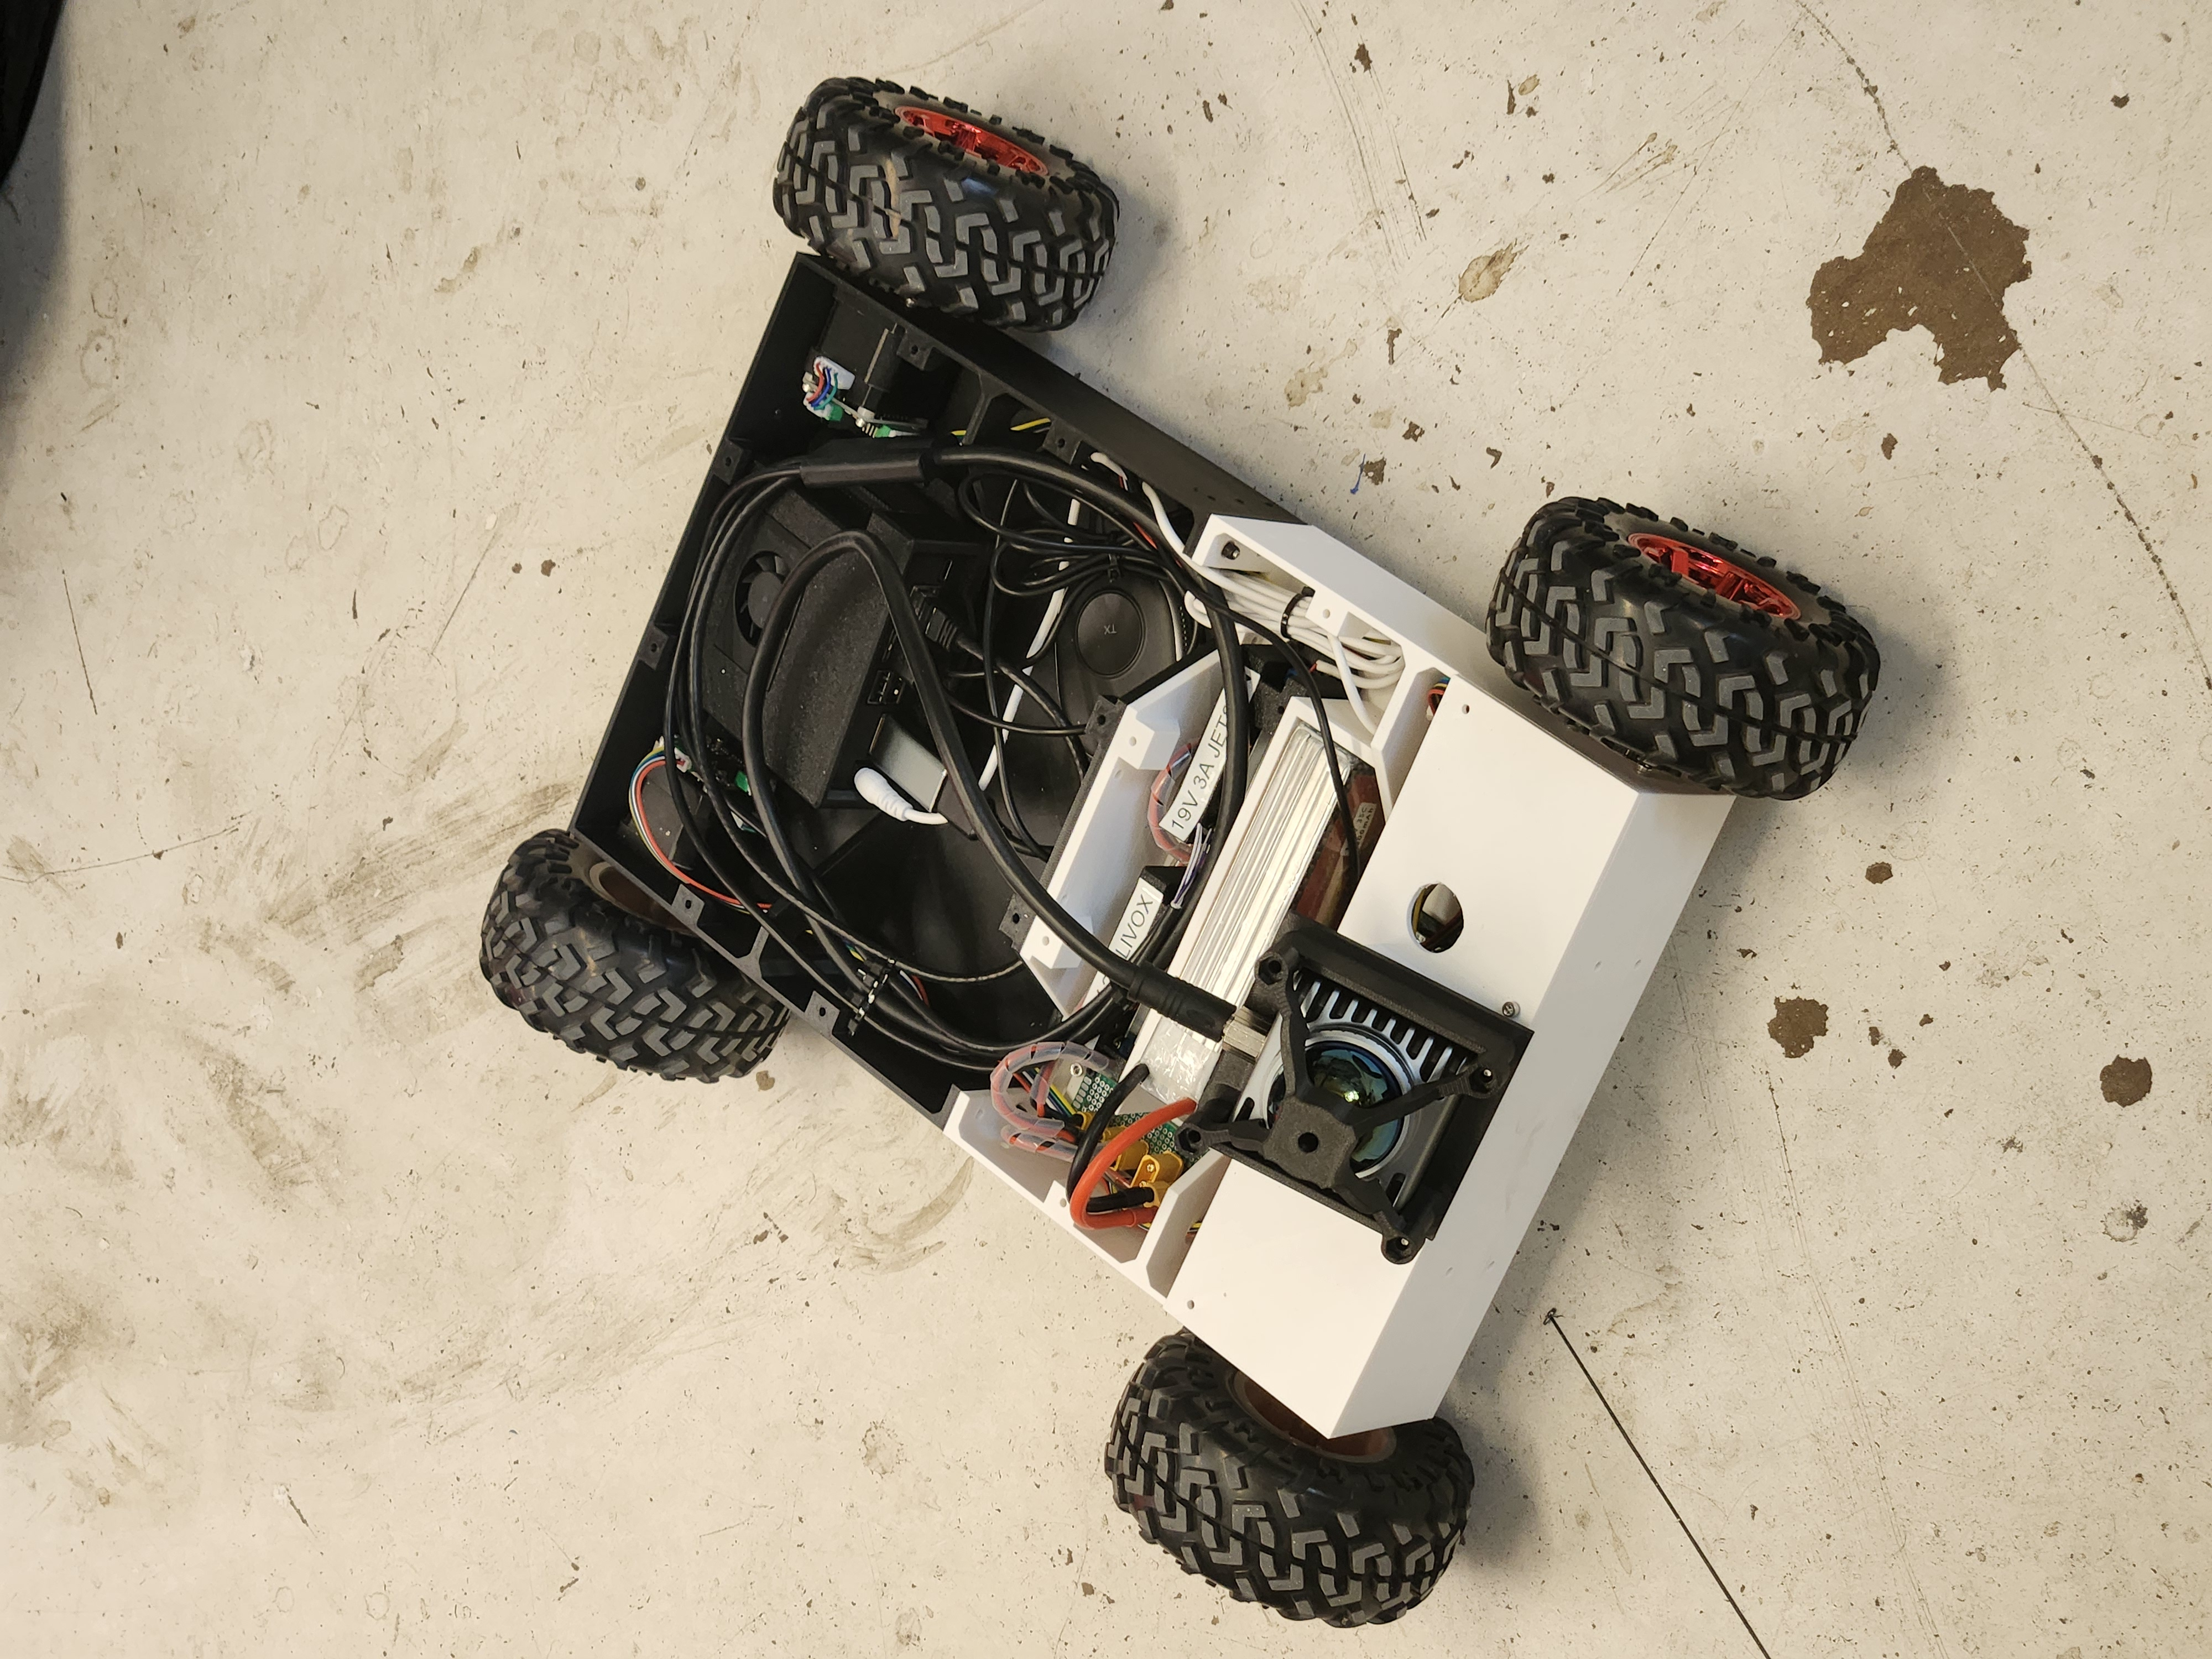
\includegraphics[width=0.4\textwidth, angle=270]{Images/roverv2openened.jpg}}       
            \caption{Rover version 1 and 2}
            \label{fig:rover_comparison}
        \end{figure}

        The new chassis is entirely 3D printed, making it fit exactly to our needs as can be seen by the CAD model in Figure \ref{fig:crawlerv2_cad}. This make the overall platform more compact and lighter. The LIDAR was also placed in the front at an angle to more easily cover the ground, which is needed for the terrain analysis that will be described in section \ref{section:terrain_analysis}. The new platform is now four wheeled, but was designed with modularity in mind to be able to add two additional wheels and motors in the center of the chassis.


        \begin{figure}[H]
            \centering
            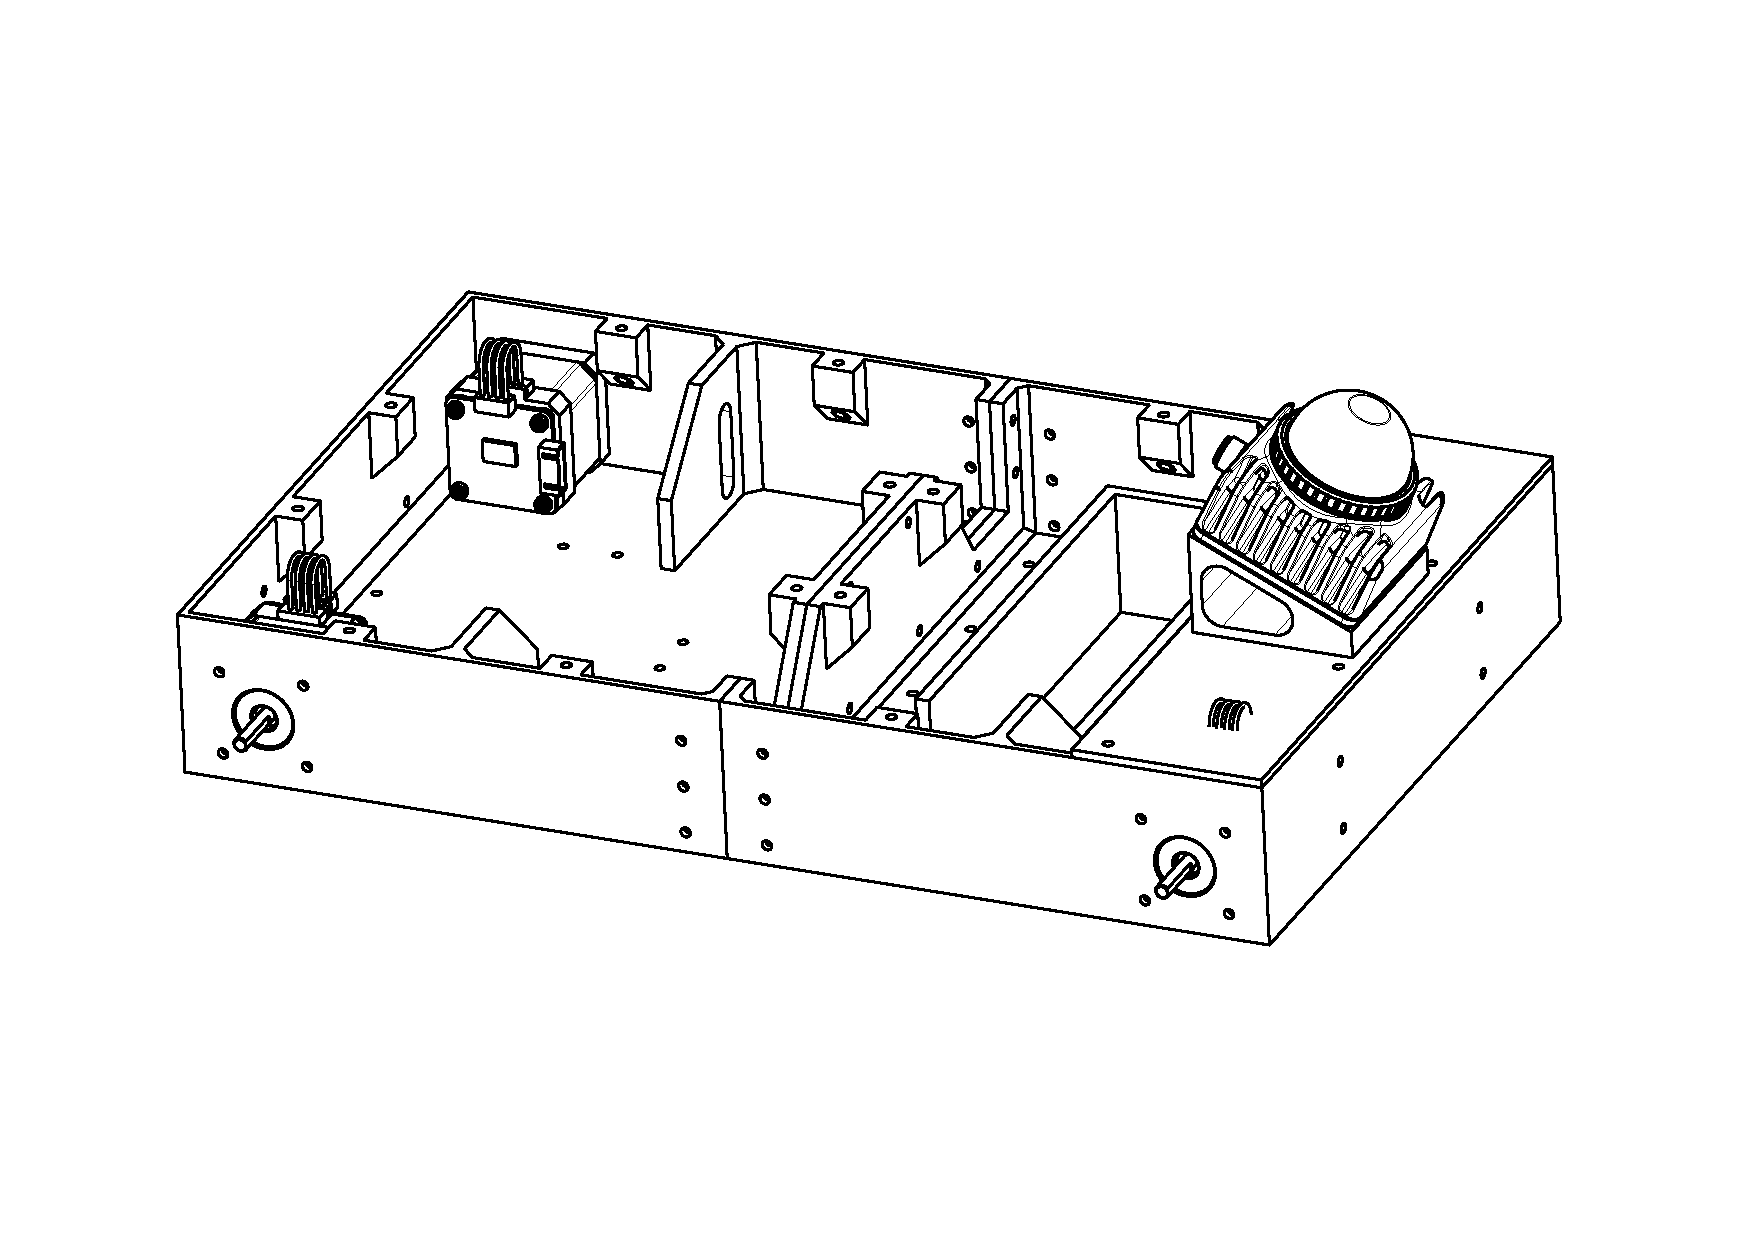
\includegraphics[width=0.8\textwidth]{Images/roverv2.pdf}
            \caption{Drawing of CAD model of the new rover with the top removed}
            \label{fig:crawlerv2_cad}
        \end{figure}


    \subsection{Quadcopter setup}
            
            % Explain the platform's starting point and the goal
            % Explain the different drones that were at my disposal and which one was selected for our application (the one that could easel;y carry the LIDAR, jetson while not being too big)

            One of the agents in our multi-agent system is a quadcopter, chosen for its ability to provide aerial perspective and navigate in three-dimensional space. After evaluating several drone options available to us, we selected a model that struck an optimal balance between payload capacity and size. This drone was capable of easily carrying the Livox Mid-360 LIDAR sensor and the Nvidia Jetson Orin embedded computer, while still maintaining a compact form factor suitable for indoor and outdoor operations.

            The quadcopter platform required several modifications to integrate our specific sensor suite and computational hardware.

            \subsubsection{Mechanical modifications}

                I designed and 3D printed new landing legs that fit on the arms of the quadcopter. Those landing legs were designed to increase the landing stability, which I noticed was a problem in the manual flight I performed, and to reduce the blind spots of the LIDAR which was to be placed in the center of the underside of the drone.

                I also took the opportunity to redesign the battery mounting mechanism which was bulky, heavy, and suitable to only one size of battery, to be much simpler and use Velcro straps as can be seen in Figure \ref{fig:landing_legs}. This resulted in a saving of around 150 grams and thus increased the flight time of the drone. The Mid-360 LIDAR was mounted on the underside of the drone, in the center, to provide a full 360-degree view of the surroundings. 
                

                \begin{figure}[H]
                    \centering
                    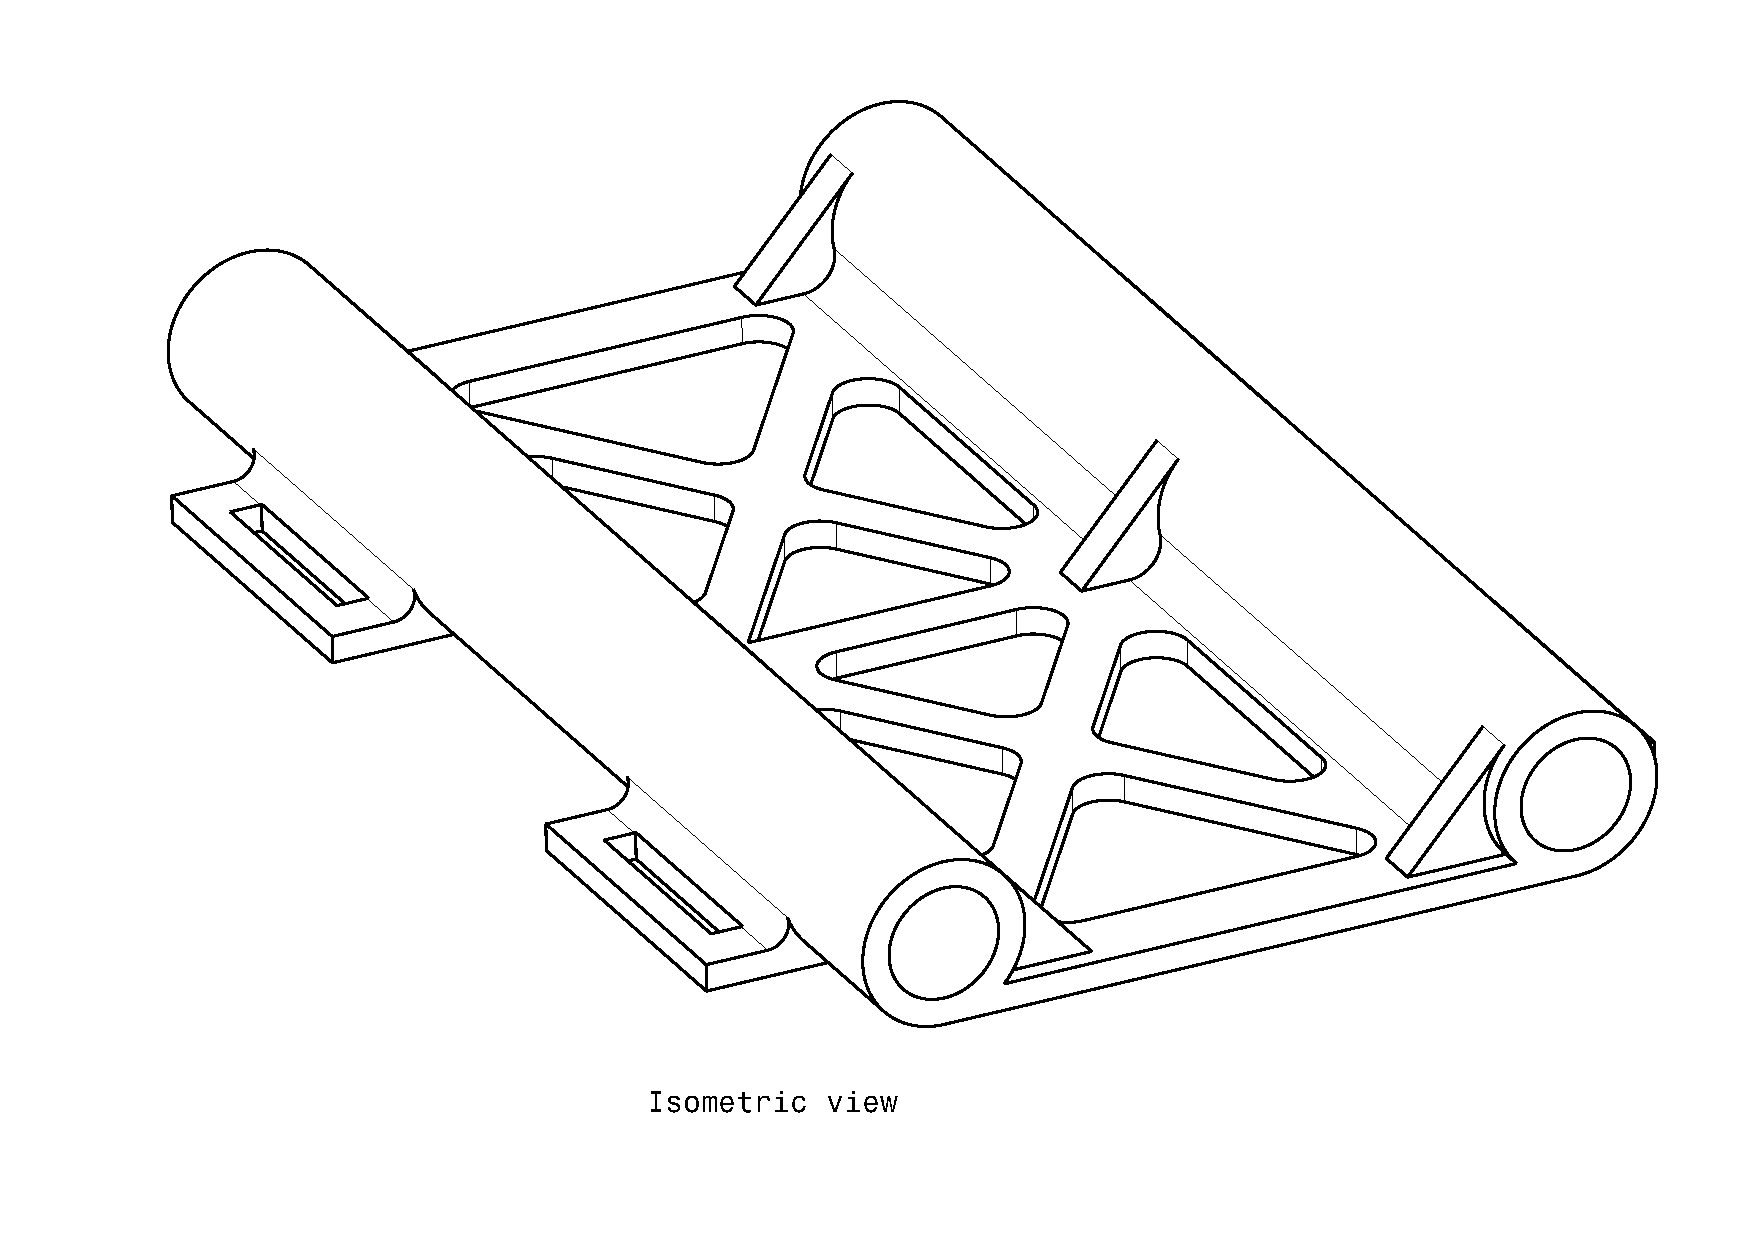
\includegraphics[width=0.6\textwidth]{Images/BatteryTrayDrawing.pdf}
                    \caption{Drawing of CAD model of new battery tray}
                    \label{fig:landing_legs}
                \end{figure}    
            \subsubsection{Electronics architecture}

                % Similarly to the rover, the jetson is still connected to the LIDAR via ethernet 
                % The drone is controlled by a PLACEHOLDER_CONTROLLER, which is connected to the jetson via USB

                To keep the architecture similar to the one used on the wheeled robot, the quadcopter was also equipped with an Nvidia Jetson Orin embedded computer and a Livox Mid-360 LIDAR. The computer and the LIDAR get their power from the drone's battery, which is regulated to 19V and 12V respectively.

            \subsubsection{Software architecture and setup}
                
                % don't know what planner to use, something complicated or just a grid coverage planner
                Time didn't allow for the implementation of a full navigation stack on the drone. As such, only a theoretical architecture, similar to the previous platform, was planned.
                
                The goal was to use a modified version of TARE planner for aerial navigation that would consider paths in 3D for the local planner, as demonstrated by the Carnegie Mellon University \cite{cao2023representation}. The embedded computer would then send the command orders to the flight computer, a Cube Orange+, via MavLINK one one of the flight computer's USB port.

                For safety reasons, an operator with a radio controller would have been required for testing, as it is required by law to have the capability to have manual control at all time and to have the drone in view. 

                As time was running out, the drone was not fully operational and only manual testing was performed.


                % TODO : add diagram of how everything should have connected
                % TODO : and explaine how far things went 
            
    \subsection{Quadruped platform setup}

        A quadruped was chosen as the third platform as it can navigate rough terrain and climb stairs. The platform chosen was the Unitree GO2, a quadruped robot with a 3D LIDAR and an embedded computer.

        \subsubsection{Compute backpack}

        Even though the Unitree GO2 has a LIDAR of its own and an embedded computer based on the Rockchip RK3588S inside, we decided to add an additional LIDAR on top of the platform and as such, we needed an additional embedded computer.

        As is the case with the wheeled platform and the drone, we chose to use a Livox Mid-360 LIDAR and a Nvidia Jetson Orin embedded computer. Even though the quadruped already carries a 3D LIDAR, we chose to use a Mid-360 as the ladder produces around ten times more points per second (21600 points per second for the Unitree L1 LIDAR against the 200000 points per second of the Mid-360).

        \begin{figure}[H]
            \centering
            \begin{minipage}{0.45\textwidth}
                The compute backpack also provides access to a power port through an Amass XT-30connector and a gigabit Ethernet port on the robot that are usually covered by a plastic cover. Those ports are covered by the handle of the GO2, but a replacement plate with holes was designed as can be seen in Figure \ref{fig:handle_cover}.
            \end{minipage}%
            \hfill
            \begin{minipage}{0.5\textwidth}
                \centering
                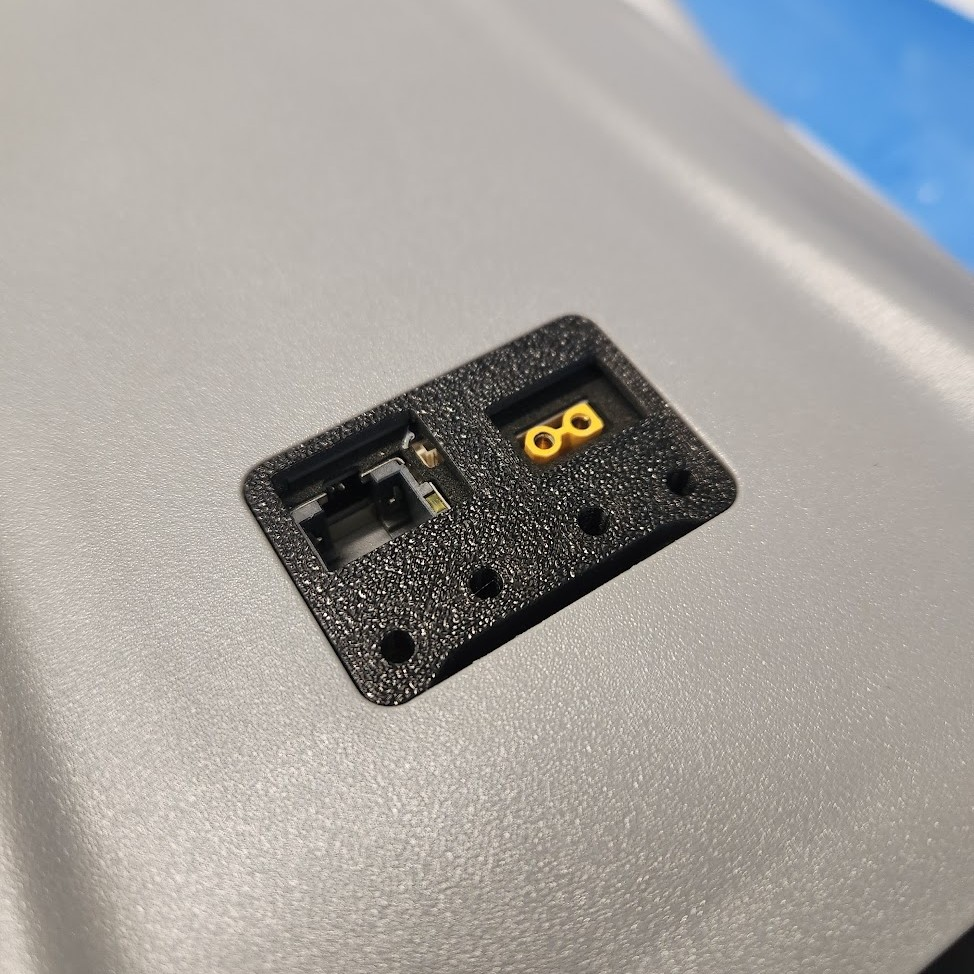
\includegraphics[width=0.75\textwidth]{Images/PortsWithCover.jpg}
                \caption{Handle and covered connectors}
                \label{fig:handle_cover}
            \end{minipage}
        \end{figure}
        To fit the Nvidia Jetson, the LIDAR, and the power regulators needed for both of them, the top part of the robot was scanned, and a new top part was designed and 3D printed. The CAD model of top part and the scan can be seen in Figure \ref{fig:scanner_and_cad}. This holds the LIDAR on the back of the robot to be sure to cover the grounds during the scanning process. The angle was determined as to not have any of the robot itself in the field of view of the LIDAR. Additionally, the compute backpack was designed to accommodate other experiments like mounting a robotic arm on the robot. For that purpose, all four sides figure threaded mounting holes.

        \begin{figure}[H]
            \centering
            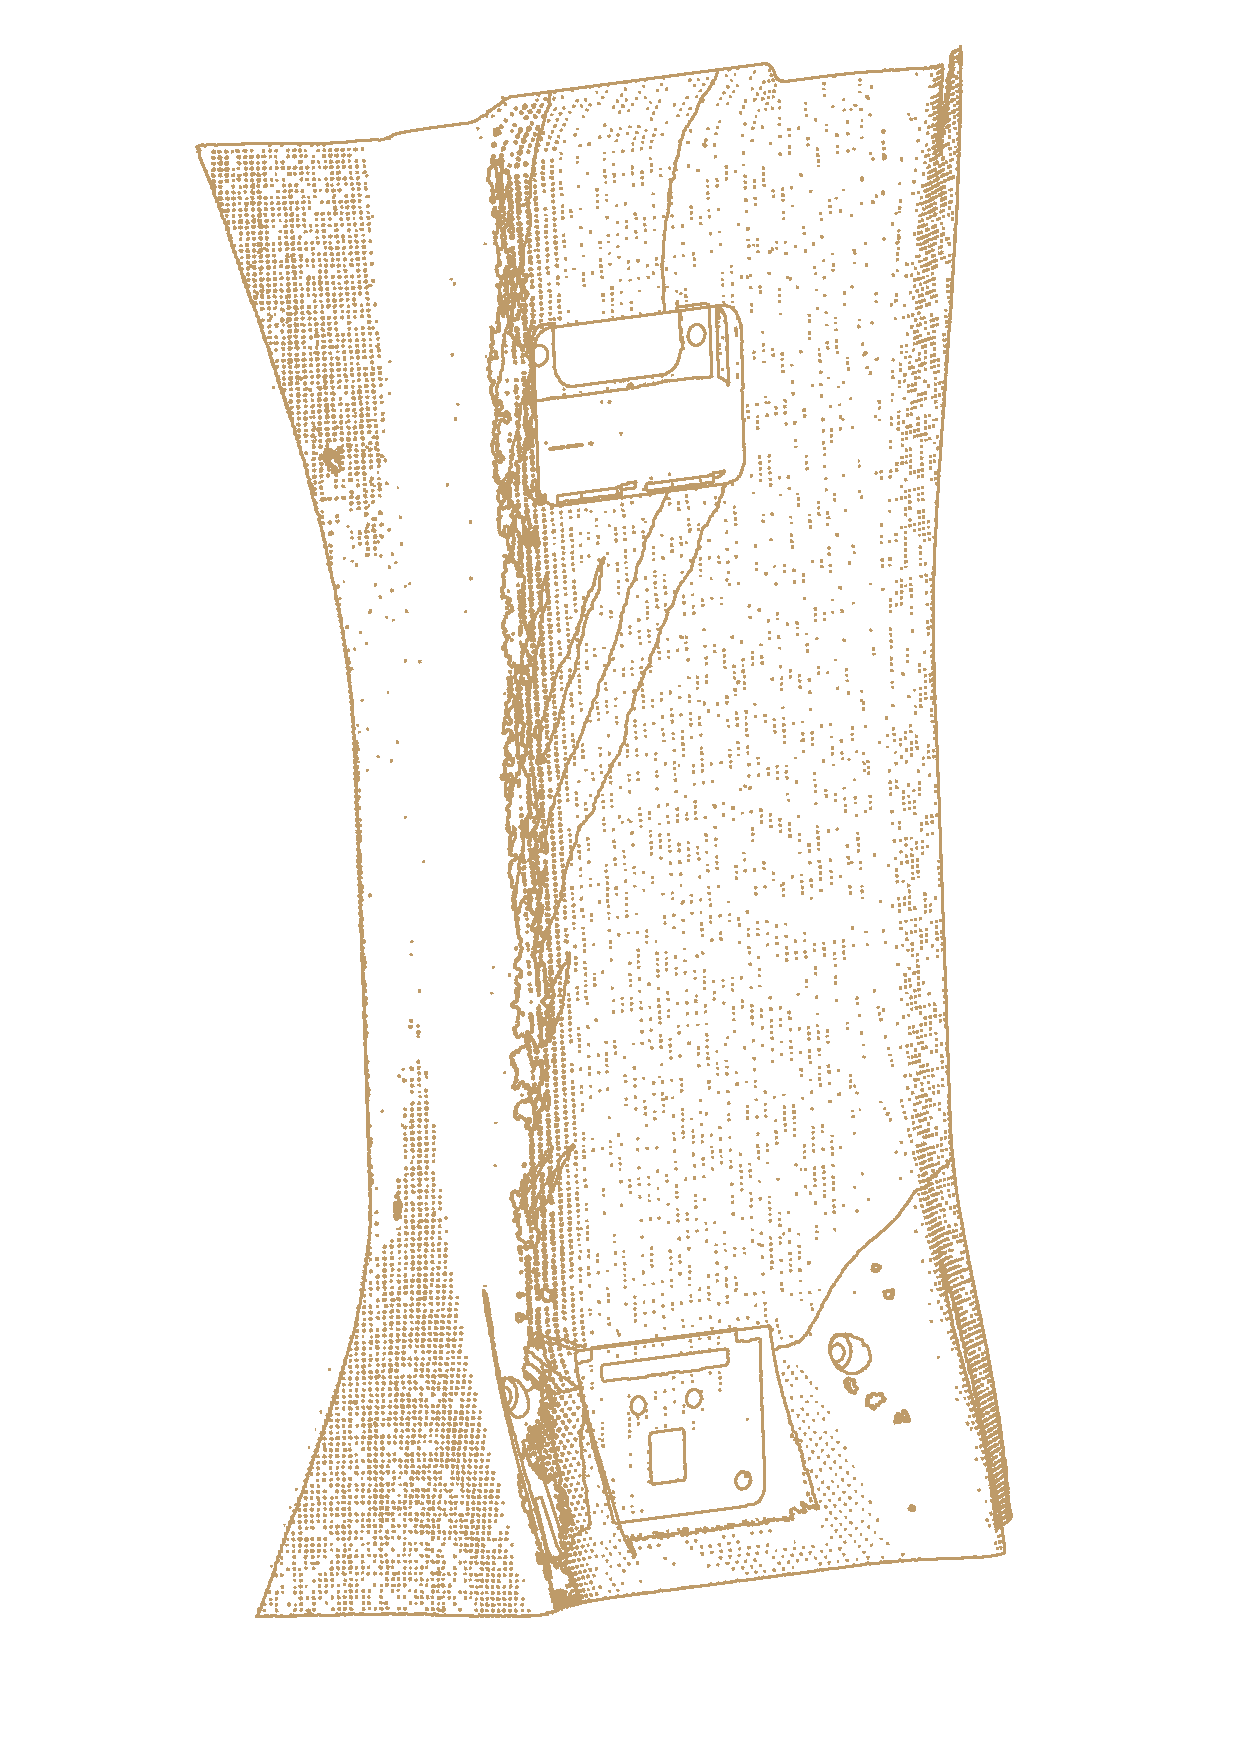
\includegraphics[width=0.3\textwidth]{Images/ScanGO2Top.pdf}
            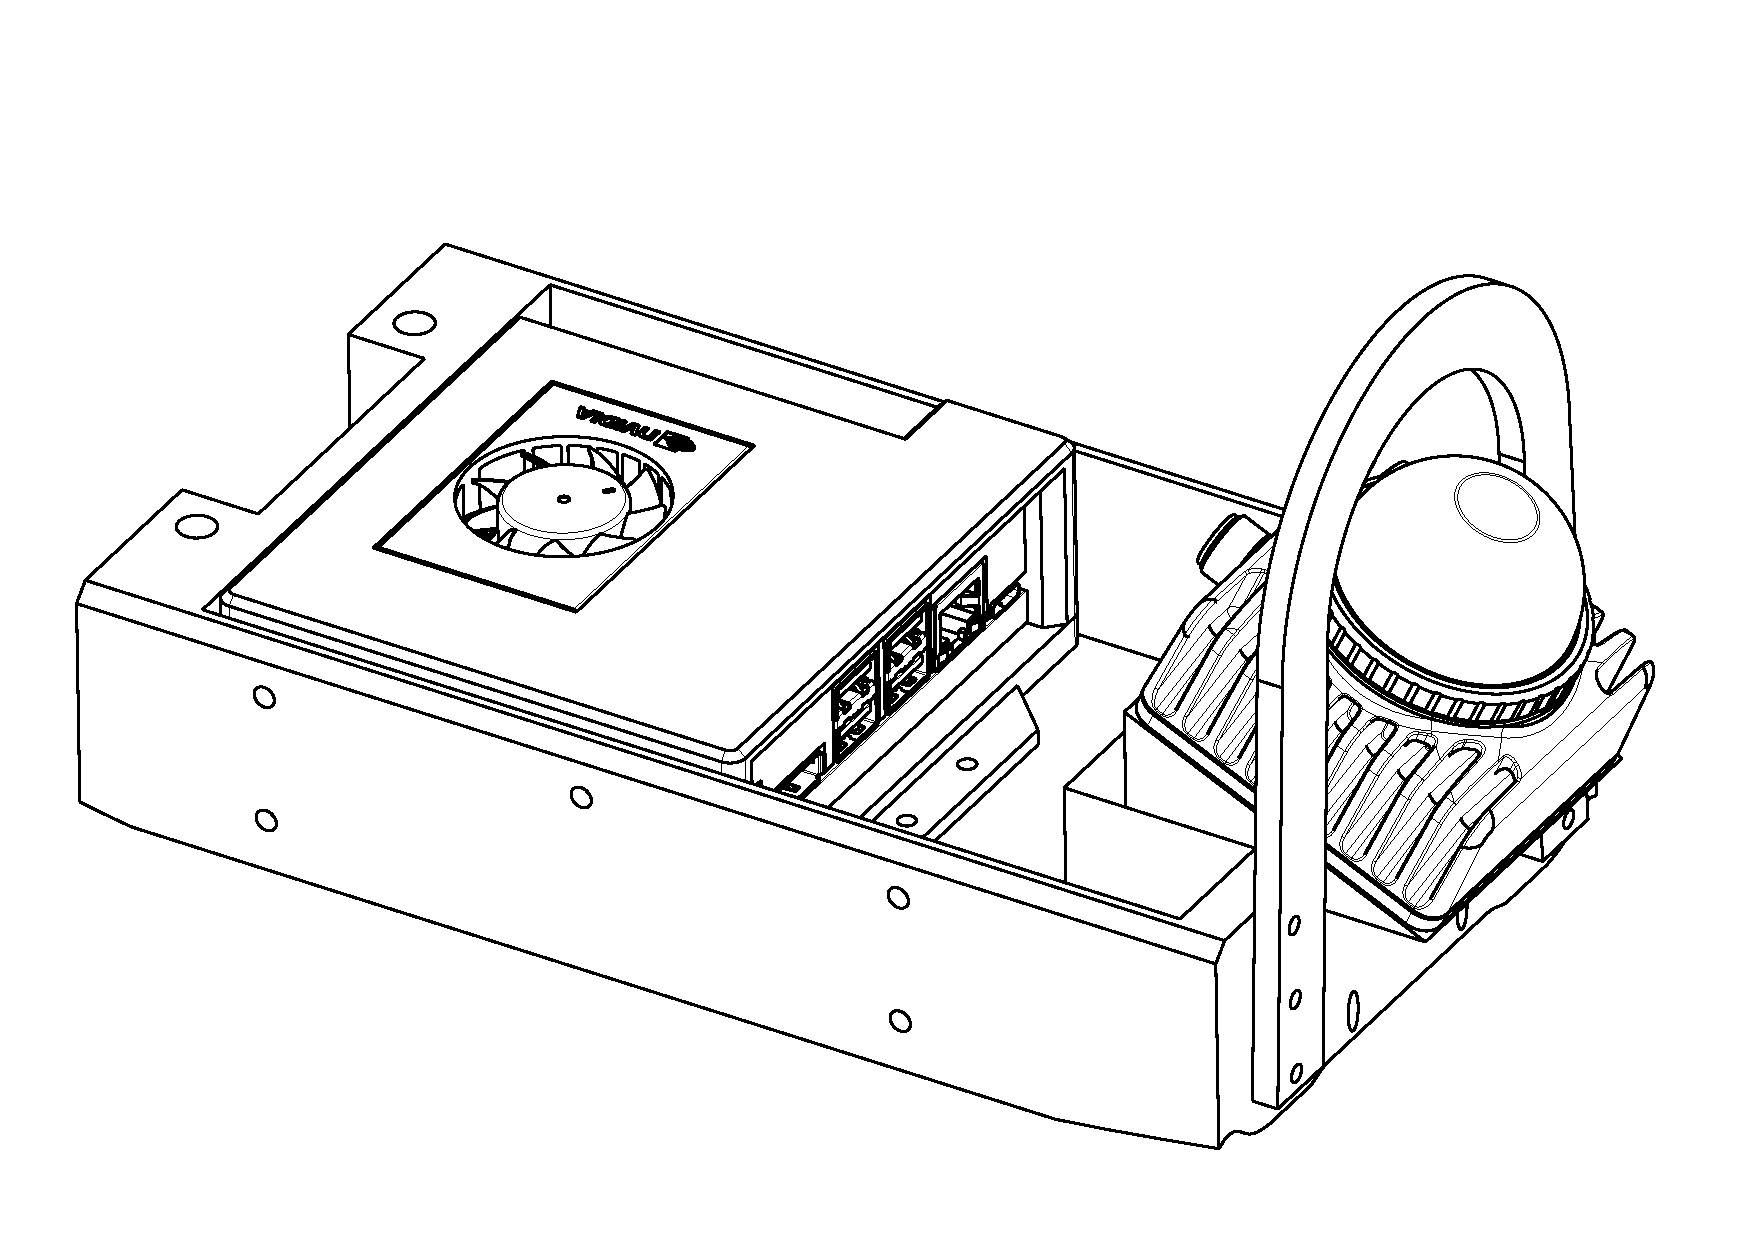
\includegraphics[width=0.6\textwidth]{Images/ComputeBackpack.pdf}
            \caption{Scanned top of GO2 robot and drawing of CAD model of the compute backpack }
            \label{fig:scanner_and_cad}
        \end{figure}

        The compute backpack's shell was 3D printed in PETG, as it is less brittle than many other filaments like PLA or ABS. This was done so that the shell be able to withstand potential falls of the robot. The compute backpack with the Jetson Orin, the Mid-360 LIDAR, the power regulators and the cabling can be seen in Figure \ref{fig:compute_backpack}. For development purposes, a video transmitter is also fitted to provide an easy way to see the Jetson's desktop without having to connect a monitor to it. As this is powered by USB, it doesn't require any additional power source.

        \begin{figure}[H]
            \centering
            \includegraphics[width=0.75\textwidth]{Images/go2_backpack.jpg}
            \caption{Compute backpack mounted on quadruped}
            \label{fig:compute_backpack}
        \end{figure}


        
        \subsubsection{Communication with the quadruped}

        To send command to the quadruped, Unitree offers a controller, a phone app, an SBUS port, a UWB remote, and an upgraded version of the robot that support CycloneDDS communication via Ethernet.

        The controller uses both Bluetooth and a longer range 2.4GHz radio to communicate with the robot. This controller is only capable of sending movement commands, predefined non-modifiable actions, and initiate calibration. The Bluetooth seems to be used for initialization but is not required at longer ranges and all control commands are sent via the 2.4GHz radio.

        The phone app uses WebRTC, a real time communication protocol commonly used for web browser communication. In the case of the quadruped, the robot can either act as an access point (AP mode) and the phone then connects to the Wifi created, or both the phone and robot can connect to an existing Wifi network in station mode (STA mode). This communication is not encrypted and thus provides an easy communication to the robot that we can emulate \cite{go2_webrtc}. Compared to the remote control, we also get information back from the robot, including but not limited to : joint angles, preprocessed LIDAR data, odometry estimation, camera feed. This communication method has the advantage that it is simple and gives us most of the data, that is why it was used for the first control tests of communication between a laptop and the robot. It however doesn't provide data at a high rate of speed at only 10 Hz for most of the data, and doesn't give access to the raw LIDAR measurements for example. It also doesn't allow us to control each joint individually if we wanted to implement additional gaits in the future.

        The SBUS, or Serial Bus, port that is present on the top of the robot is meant for use with long range radio controllers, often used in radio controlled drones. This only gives us high level control of the movement and does not provide any data back.

        The UWB, or Ultra Wide Band, remote is an optional feature of the robot that provides the capability of person following to the robot. This remote also features a small joystick for manual control and uses the same technologies as the main controller. The UWB uses multiple antennas in the robot to estimate the position of the tracker that a person carries, giving a rough estimation of the position of the remote which the robot can then follow. However, this is not something that will help us in the control of the robot.

        Finally, the robot also features an Ethernet port, connected to the internal computer, as can be seen in Figure \ref{fig:handle_cover}, and as will be discussed in section \ref{section:go2_battery} this can provide a Data Distribution Service (DDS) using the CycloneDDS protocol. This protocol was developed by Eclipse and is an implementation of the Object Management Group (OMG) DDS. This protocol is used in many industrial applications and is known for its low latency and high reliability. CycloneDDS is one of the ROS MiddleWares (RMW) that can be used, and it is often praised for it's low latency and low CPU and memory usage. This way of communicating also offers the most control from very low level commands of each joint and raw LIDAR data, up to high level commands like predefined gaits and actions defined by Unitree. This is the communication method that we will use for the final implementation of the project.
    

        \begin{figure}[H]
            \centering
            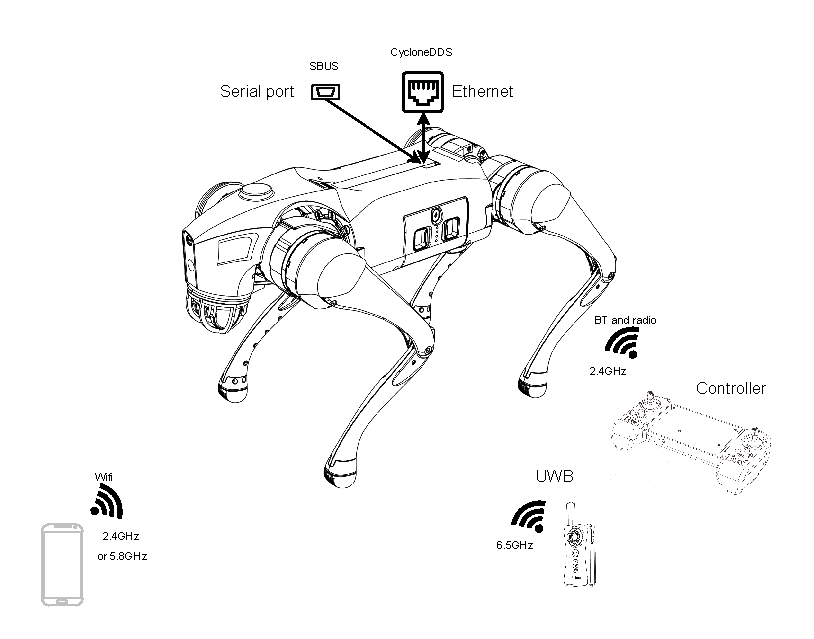
\includegraphics[width=0.8\textwidth]{Images/go2-communication.pdf}
            \caption{Communication methods with the GO2 robot}
            \label{fig:go2_communication}
        \end{figure}

        % explain how we use webRTC to communicate with the robot (explain whatit is and how it works)
        % explain how we could use the cycloneDDS because we have access to the newly jailbreaked robot
        
    \subsection{Issues encountered}
        \label{section:go2_battery}
        %Big battery issue, reverse engineering of the battery, jailbreaking of the robot
        As delivered, the robot was not functional as the battery was discharged beyond the point of no return. The battery was disassembled (see Figure \ref{fig:disassembled_battery}) and partly reverse engineered to understand the problem. Even though the battery was not repairable, the reverse engineering allowed us to understand the battery's BMS and how it communicated with the robot. In Table \ref{table:battery_protocol} it can be seen that I was able to partly reverse engineer the battery communication protocol. This was shared with others from the open source community actively trying to design a replacement motherboard for the robot. The battery was then replaced by a new one and offered around two hours of walking with the LIDAR and the Jetson Orin powered on.

        \begin{figure}[h]
            \centering
            \subfigure[Disassembled battery]{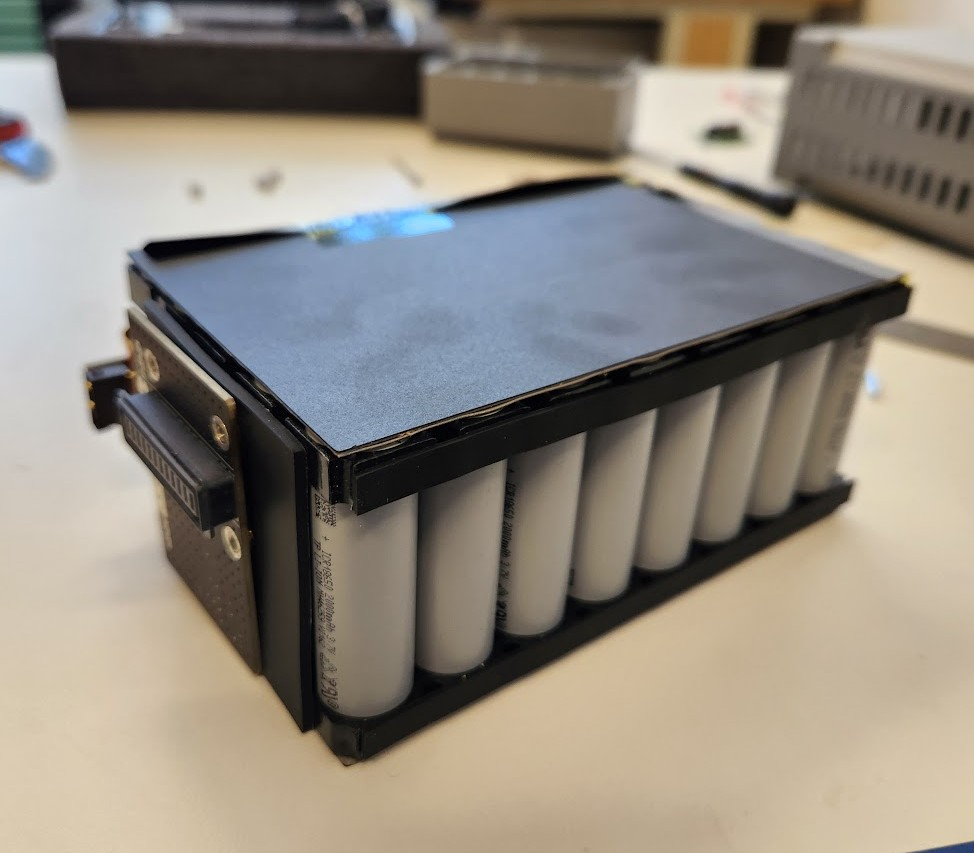
\includegraphics[width=0.4\textwidth]{Images/teardown_battery.jpg}}
            \subfigure[Battery Management System (BMS)]{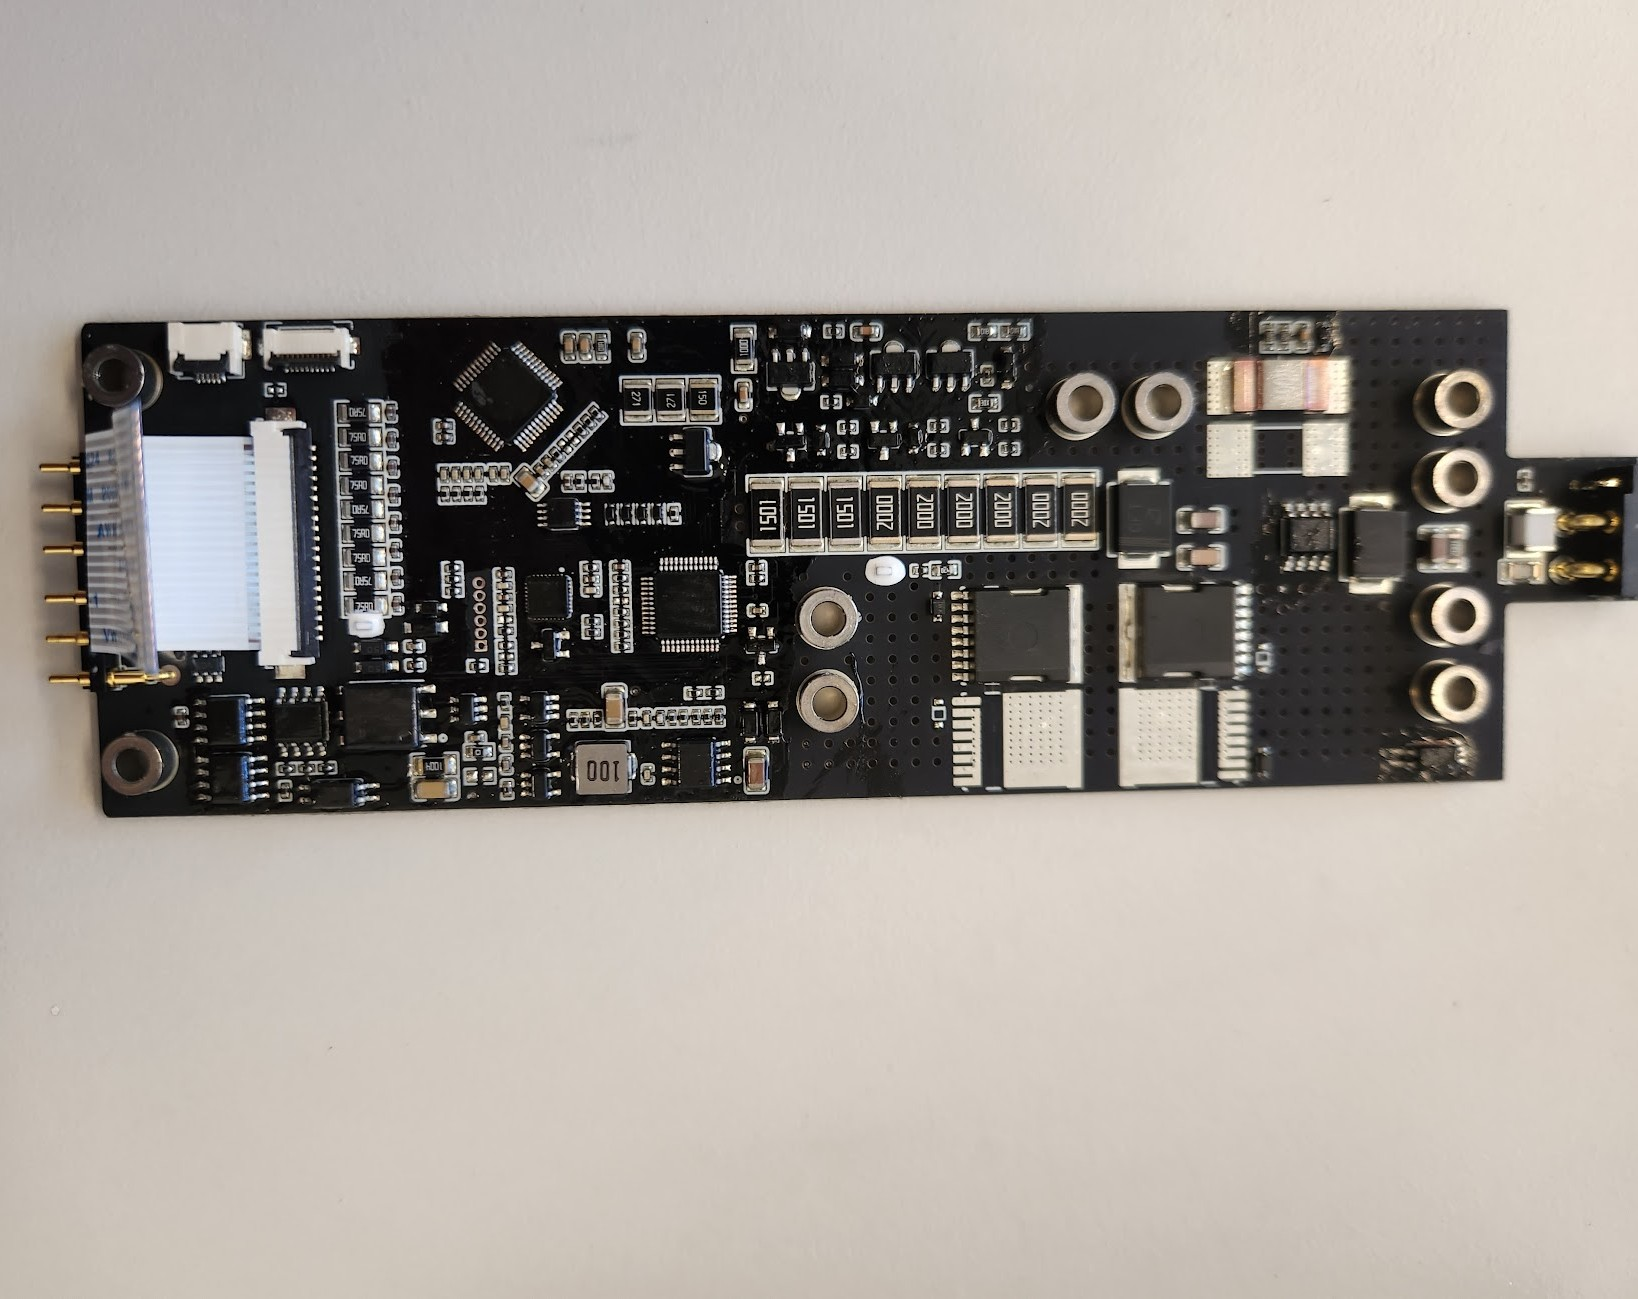
\includegraphics[width=0.44\textwidth]{Images/BMS.jpg}}
            \caption{Disassembled battery and Battery Management System (BMS)}
            \label{fig:disassembled_battery}
        \end{figure}

        \begin{table}
            \centering
            \begin{tabular}{|c|c|c|c|}
                \hline
                Byte & Data & Conversion & Comment \\
                \hline
                0 & EF FE & -4098 & start of battery message \\
                2 & 3C 03 & 15363 & start of battery message \\
                4 & 0F 00 & 3840 & cell 8 voltage in mV \\
                6 & 0F 01 & 3841 & cell 7 voltage in mV \\
                8 & 0F 01 & 3841 & cell 6 voltage in mV \\
                10 & 0F 03 & 3843 & cell 5 voltage in mV \\
                12 & 0F 01 & 3841 & cell 4 voltage in mV \\
                14 & 0E FF & 3839 & cell 3 voltage in mV \\
                16 & 0F 01 & 3841 & cell 2 voltage in mV \\
                18 & 0F 01 & 3841 & cell 1 voltage in mV \\
                20 & 77 FB & 30715 & battery total voltage in mV \\
                22 & 01 29 & 297 &  \\
                24 & FF F8 & -8 &  \\
                26 & FF FF & -1 &  \\
                28 & 64 00 & 100 & SoC in percent \\
                30 & 09 BF & 2495 & temperature 24.95 C \\
                32 & 09 C6 & 2502 & temperature 25.02 C \\
                34 & 09 A4 & 2468 & temperature 24.68 C \\
                36 & 09 A8 & 2472 & temperature 24.72 C \\
                38 & 00 00 & 0 &  \\
                40 & 57 70 & 22384 &  \\
                42 & 09 01 & 2305 & number of charge or discharge cycles \\
                44 & 0D 06 & 333 &  \\
                46 & 00 00 & 0 &  \\
                48 & 00 00 & 0 &  \\
                50 & 00 00 & 0 &  \\
                52 & 00 FF & 255 &  \\
                54 & 00 00 & 0 &  \\
                56 & 47 80 & 18304 & crc32 \\
                58 & 7E 9D & 32413 & crc32 \\
                \hline
                \end{tabular}
                \label{table:battery_protocol}
            \caption{Partly decoded battery protocol}
        \end{table}


        One of the other issues encountered happened after a software update of the robot. We weren't able to connect via SSH to the Linux computer inside the robot. This required many days of reverse engineering of the new firmware with the help of other people online.

        The update had removed a vulnerable update mechanism that previously allowed us to gain a root shell to the robot. With that shell, we were then able to change the password of the robot and gain access to the robot via SSH. The new firmware had also prevented us from using the Ethernet port of the robot to communicate to the robot using the CycloneDDS which is one of the Data Distribution Services that ROS can use. This functionality of the robot is usually reserved for the educational version of the GO2, but the company doesn't offer any upgrade from the standard version to the educational version.

        As such, I helped the open source community to design a new unlocking method. For reference, in the previous version, only a version number in a single file needed to be changed from a 2 to a 4 to unlock every functionality of the robot. The new update brought many new challenges as every binary was now heavily obfuscated and had increased in size by a factor of 10, every file's checksum was now verified by a yet unknown program, no debugger could be attached as every binary checked their parent process, and many other obfuscation techniques were used.

        The anti debugger technique was quickly bypassed as only the name of the parent process was checked against a list of names, \texttt{gdb-server} not being part of this list made it easy to debug the binaries. Every binary also checked for the presence of a \texttt{tracepid} value, which was solved at first with kernel module that hides the presence of the \texttt{tracepid} value. Other threads were also created to continue monitoring those values in the binaries, but patching the \texttt{pthread\_create} instructions to \texttt{MOV X0, \#0} solved that problem.

        Once the location of the checksum check was identified in a binary, the instruction responsible for the comparison was patched to always return true : the previous instruction \texttt{BL <compare>} was replaced by \texttt{MOV X0, \#0}.

        Finally, the version check was bypassed by consolidating two instruction in one, to in terms have room to set the value of the register \texttt{X0} to 4 as can be seen in Table \ref{tab:patched_instructions}.
        

        % Please add the following required packages to your document preamble:
        % \usepackage[table,xcdraw]{xcolor}
        % Beamer presentation requires \usepackage{colortbl} instead of \usepackage[table,xcdraw]{xcolor}
        \begin{table}[]
            \centering
            \mbox{}\clap{
            \begin{tabular}{|l|l|l|l|l|}
            \hline
            \textbf{Address} & \textbf{Original value} & \textbf{Original Instruction}      & \textbf{Patched value} & \textbf{Patched instruction}       \\ \hline
            \texttt{565BD80} & \texttt{E0 7B BF A9}   & \texttt{stp     x0, x30, {[}sp,\#-0x10{]}!} & \texttt{80 00 80 D2}            & \texttt{mov x0, \#4}                    \\ \hline
                                & \texttt{63 4D 00 94}   & \texttt{bl      sub\_566F310              } & \texttt{E0 7B BF A9}            & \texttt{stp x0, x30, {[}sp,\#-0x10{]}!} \\ \hline
                                & \texttt{84 00 00 18}   & \texttt{ldr     w4, \#0x565BD98           } & \texttt{63 4D 00 94}            & \texttt{bl sub\_566F310}                \\ \hline
                                & \texttt{84 7C 40 93}   & \texttt{sxtw    x4, w4                    } & \texttt{64 00 00 98}            & \texttt{ldrsw X4, \#0x565BD98}          \\ \hline
            \end{tabular}
            }
            \label{tab:patched_instructions}    
            \caption{Patched instructions for version check}
        \end{table}




    \newpage

\section{Mapping, planning, and exploration}

    There are three main components to the software architecture of the multi-agent system: mapping, planning, and exploration. Mapping first involves knowing where the robot is and how it is moving, or it's odometry. Planning is often divided in two scales, a local one where we consider what movements the robot is capable of doing, a global one that aims to find the best path to a distant goal. Exploration uses the two former process to determine where the robot should go to maximize the information gathered.

    \subsection{Mapping}

        Mapping is the action of aligning the robot's acquired LIDAR scans in relation to the initial pose. For that, one or multiple methods of odometry are needed. 
        \subsubsection{Introduction to SLAM}
        SLAM or Simultaneous Location And Mapping is the action of using a scanner, in our case a LIDAR, for both the construction of a map, and utilizing this map to infer our position. In 2D, algorithms like Monte Carlo based particle filters \cite{fox1999monte}, or graph based approaches \cite{macenski2021slam} are used and have not been lately improved. In 3D, the problem is much more complex and the algorithms are much more computationally expensive. 
        
        When using SLAM as an odometry method, problems like drift can occur. As can be seen in Figure \ref{fig:scan_basement}, the drift of the odometry can be seen in map acquired in a large basement : a doubling of the corridors one the right of the image can be seen. This drift is due to inaccuracies in the odometry, often acquired in areas with few features to align the scans to. This can be remedied with methods that use loop closure \cite{chen2021inertial} \cite{liu2022enhanced}.

        \begin{figure}[H]
            \centering
            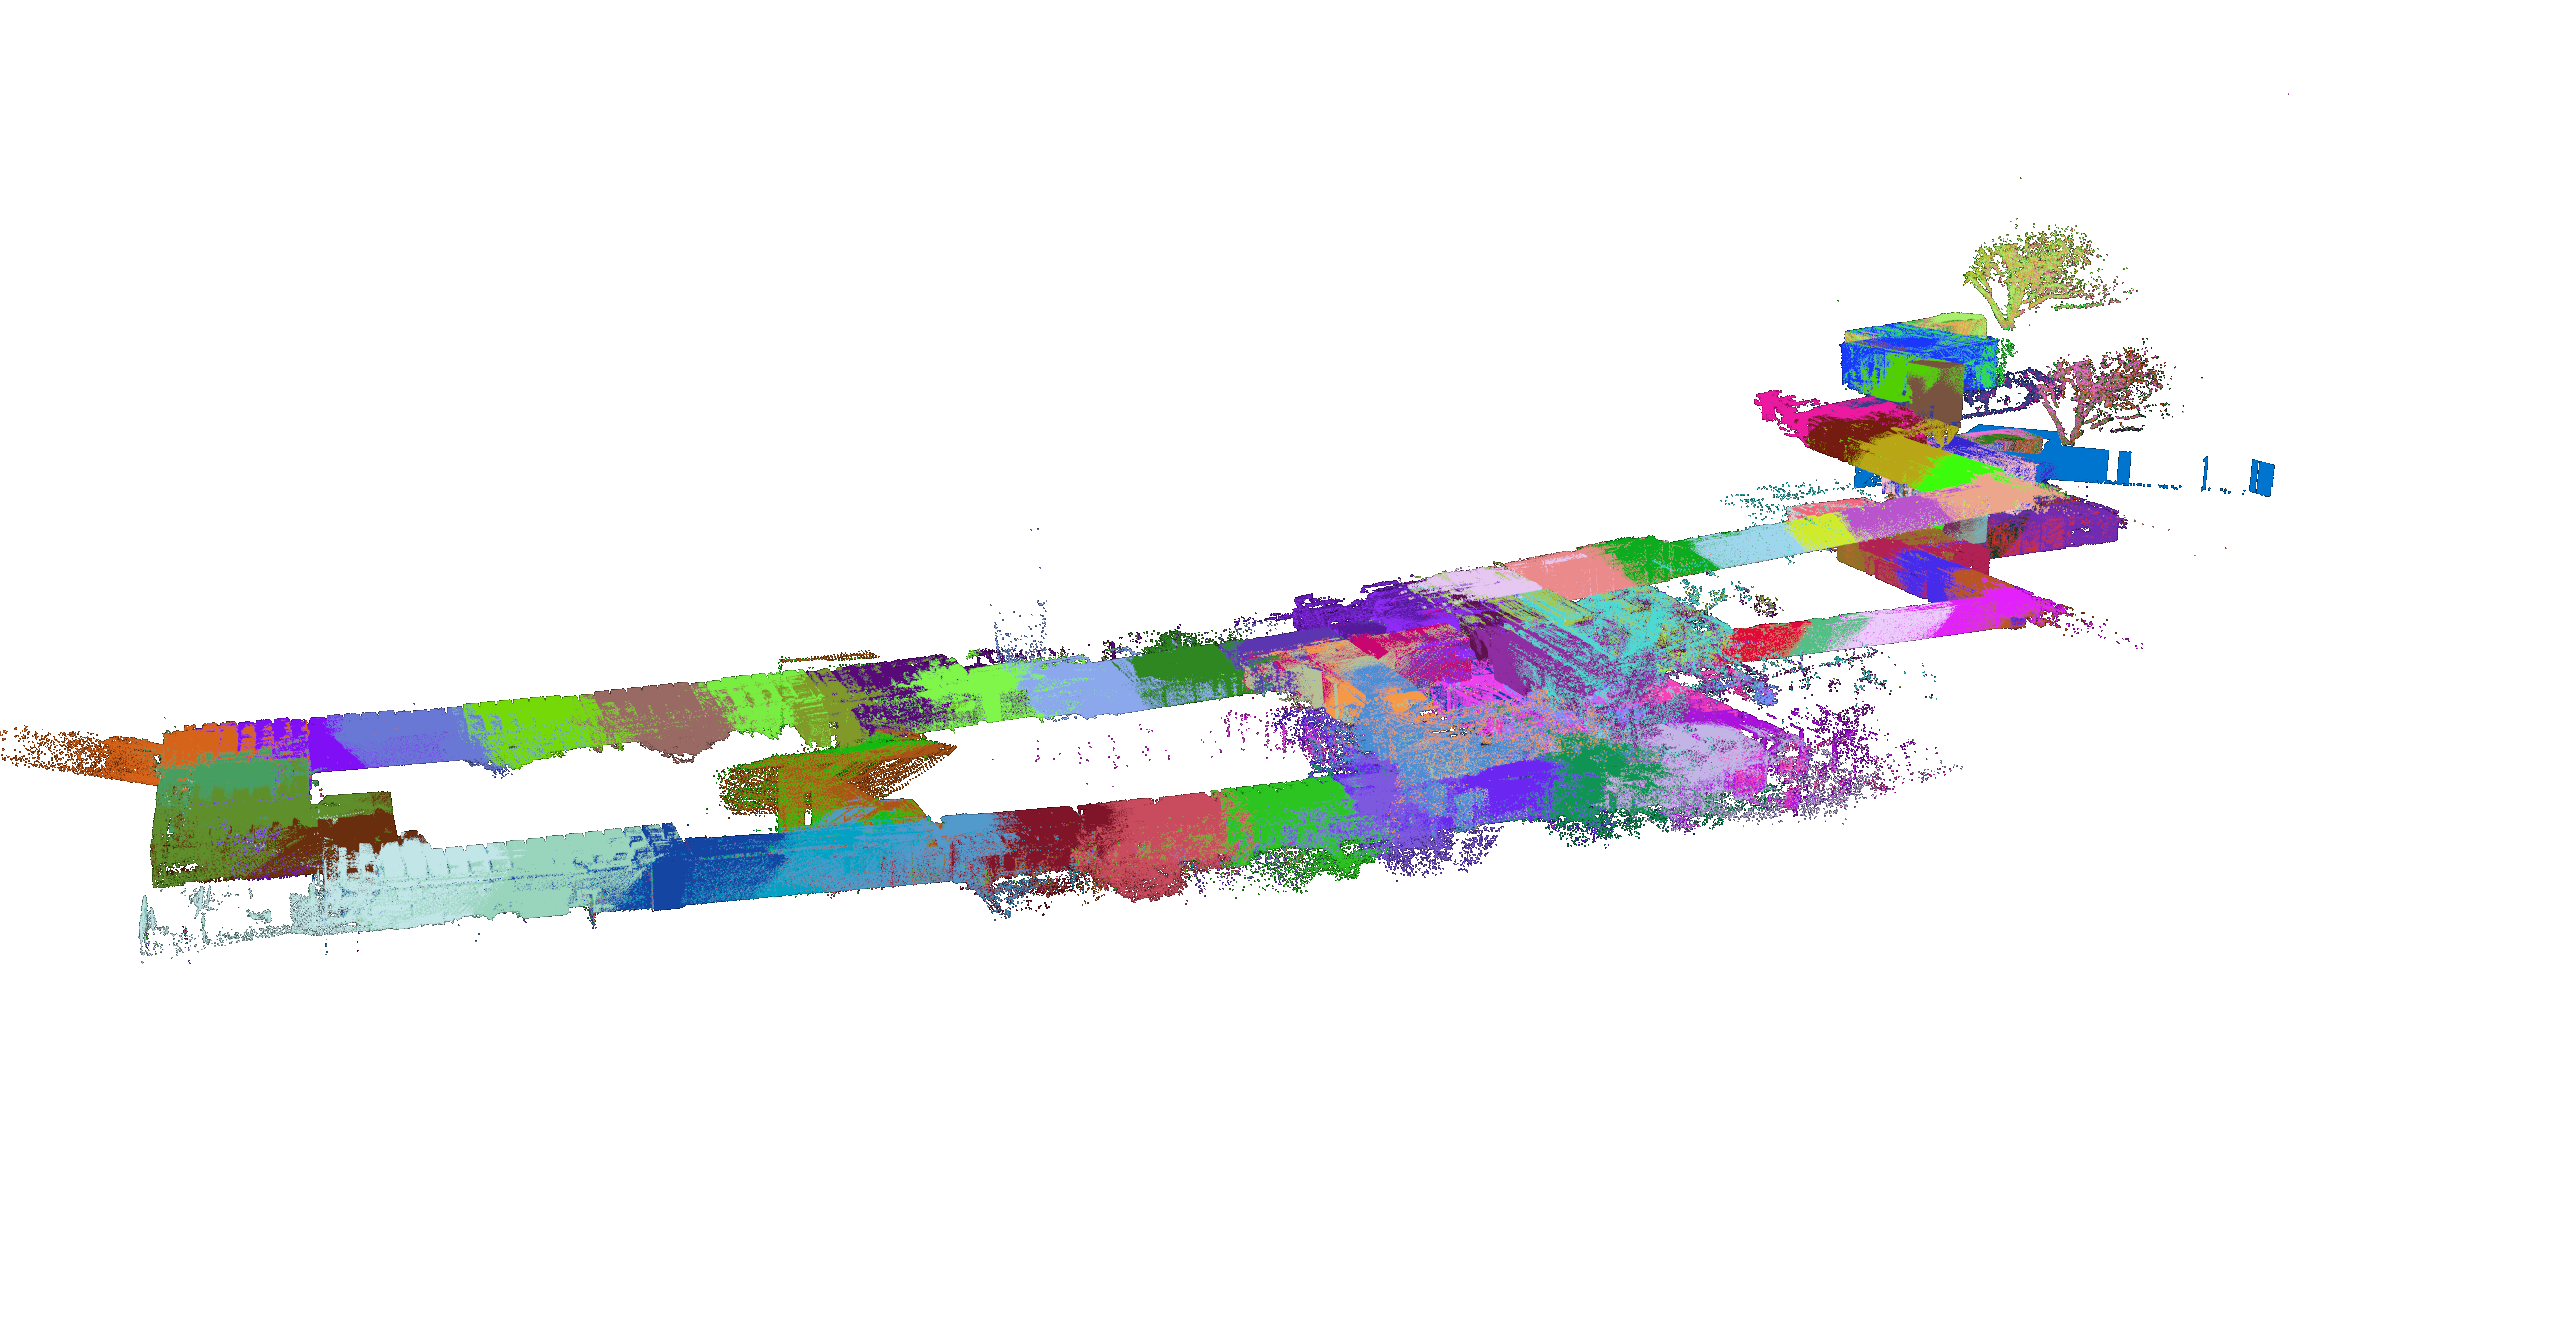
\includegraphics[width=0.9\textwidth]{Images/scan_basement_no_bg.png}
            \caption{Scan of a large IIT basement (150m in length) showing the drift of the odometry. Each color represents a 10s scan.} 
            \label{fig:scan_basement}
        \end{figure}

        \subsubsection{LIDAR inertial odometry}
        \label{section:lidar_inertial_odometry}
        LIDARs are often paired with Inertial Measurement Units (IMUs) as algorithms can be conceived to make use of both the LIDAR and the IMU for odometry. Registration of features of the last scan of the LIDAR with previous ones provide long term accuracy and minimize potential drift, while the IMU provide a high rate of movement data that can be used to both facilitate the alignment, as well as to undistort or unskew the scans that were captured during fast movements.
        
        As the Livox Mid-360 also carries an IMU, this is the reason why I turned myself to those kinds of algorithms for the odometry. 
        
        One such algorithm is FAST-LIO2 \cite{xu2022fast}, which I chose for being close to the state of the art and having a version available that was compatible with the Mid-360 LIDAR. A more detailed comparison of the different LIDAR inertial odometry algorithms will be presented in the section \ref{section:etatArt}. The steps this algorithm takes are shown in Figure \ref{fig:fastlio2}, taken from the paper. As an implementation of the algorithm was available, I did not have spend enough time to understand every step of it, but a state of the art of LIDAR inertial odometry algorithms will be presented in the next section to understand what were the improvements of FAST-LIO2 over previous works.
        
        \begin{figure}[h]
            \centering
            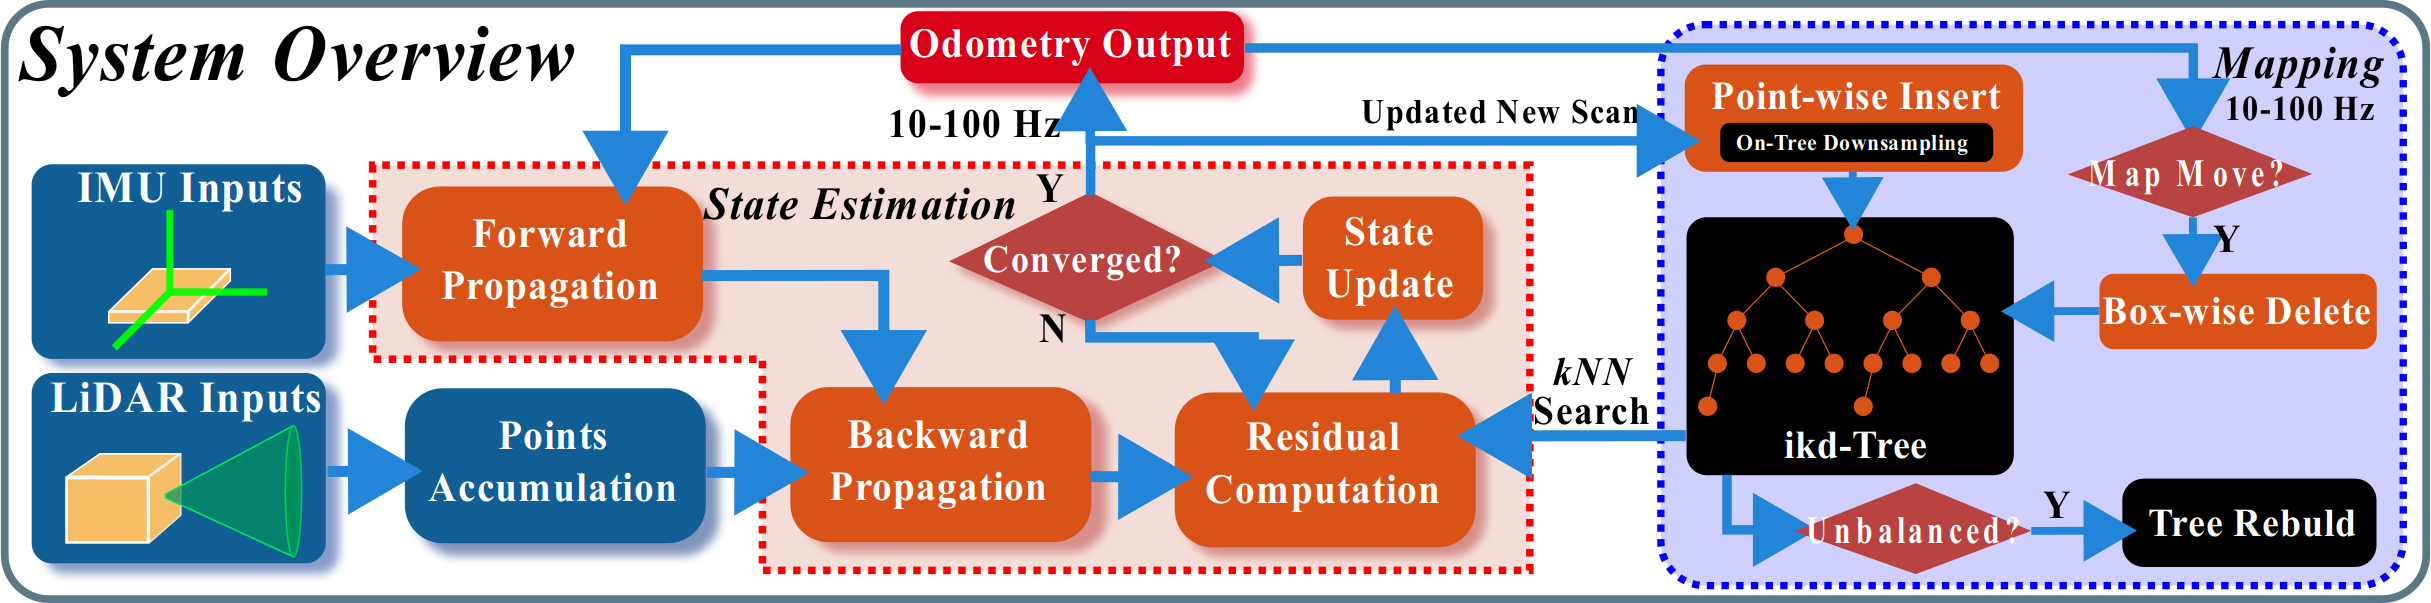
\includegraphics[width=0.95\textwidth]{Images/overview_fastlio2.png}
            \caption{FAST-LIO2 algorithm description taken from \cite{xu2022fast}}
            \label{fig:fastlio2}
        \end{figure}
        
        \subsubsection{Comparison of LIDAR inertial odometry algorithms}

        I chose to compare LIDAR inertial odometry algorithms as it is the sensor readings available to us. LIDAR inertial odometry algorithms can be divided in two categories based on how the LIDAR and IMU data are fused : loosely coupled and tightly coupled.

        Loosely coupled methods estimate the state of each sensor independently, combines the measurement with weights, and then determines the position of the robot. Those methods are useful when both sensors are independent and changes to them want to be tested. The weights can also be changed depending on the sensors used and on their accuracy and noise, or dynamically if a sensor fails or malfunctions. However, we have a LIDAR package that integrates an IMU, making the aforementioned benefits not relevant to us.

        Tightly coupled methods, on the other hand, use the measurements of all sensors to estimate the robot's position. This can mean using the IMU readings to pre process the LIDAR measurements. Those methods however require a more complex algorithm and can be more computationally expensive. They can also be more prone to failure as the failure of one sensor entails the failure of the odometry system.


        LOAM (LIDAR Odometry And Mapping) \cite{lee2024lidar} was the first loosely coupled method to be proposed and offered low computational requirements. It used the IMU measurements to estimate velocity while the LIDAR measurement used the velocity estimation for undistortion to offer better position estimation. LeGo-LOAM \cite{shan2018lego} improved on the works of LOAM by improving the performance of the pose estimation and by adding ground segmentation, making the method more robust in ground based applications.

        As for tightly coupled methods, one of the first to be proposed is in the Zebedee paper \cite{bosse2012zebedee} and showed the great accuracy tightly coupled methods can offer. It demonstrated stable mapping of a scene by placing a 2D LIDAR on a spring mobile base. LIPS \cite{geneva2018lips} formalized the closest point plane representation and added IMU preintegration for more accurate pose estimation. Ye et al. \cite{ye2019tightly} added joint optimization of the LIDAR and IMU measurements, improving the performance in high drift scenarios in long term mapping. This paper also added a rotation-contrained refinement which improves the consistency of the global map.
        FAST-LIO \cite{xu2021fast} greatly improved the performance of previous works by introducing the use of a tightly coupled iterated Kalman Filter. The high computing efficiency of the proposed gain calculation formula improves the performance, making this method interesting for real time applications on embedded systems. FAST-LIO2 \cite{xu2022fast} improved on FAST-LIO by getting rid of the feature extraction step and replacing it with a registration to the global map. It also improved performance by switching to an incrementally updated kd-tree data structure for map storage. 
        POINT-LIO \cite{he2023point} employs a different method to the previously mentioned algorithms by using a point-wise position estimation, providing a much higher frequency of odometry updates. As far as I am aware, this is the method used by Unitree in the GO2 for the LIDAR odometry they perform.

        \label{section:etatArt}


        \subsubsection{Terrain analysis}
        \label{section:terrain_analysis}
        % explain the two terrain analysis we do on the acquired point cloud

        To determine the navigable and non-navigable areas, the aligned point cloud gathered by the LIDAR and the odometry are analyzed. The first analysis is done at a close range, while the other has a longer range and a longer decay time. The topics that the two analysis subscribe and publish to are shown in Figure \ref{fig:terrain_analysis}. The extended range analysis is used by some planners to determine the best path to take while the close range analysis is used to determine the immediate surroundings of the robot as is showcased in Figure \ref{fig:terrain_analysis_comparison}.

        % The following figure shows that both terrain_analysis and terrain_analysis_ext 
        % subscribe to /odom, /registered_scan and publish /terrain_map and /terrain_map_ext respectively.
        \begin{figure}[H]
                \centering
                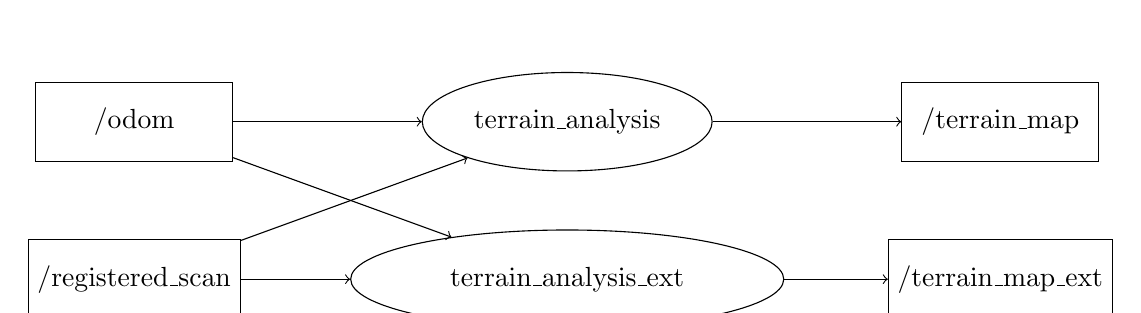
\begin{tikzpicture}[node distance=2cm, auto]
                        % Nodes
                        \node (odom) [draw, rectangle, minimum width=2.5cm, minimum height=1cm] {/odom};
                        \node (scan) [draw, rectangle, minimum width=2.5cm, minimum height=1cm, below of=odom] {/registered\_scan};
                        \node (ta) [draw, ellipse, minimum width=2.5cm, minimum height=1.25cm, right of=odom, node distance=5.5cm] {terrain\_analysis};
                        \node (ta_ext) [draw, ellipse, minimum width=5.5cm, minimum height=1.25cm, below of=ta] {terrain\_analysis\_ext};
                        \node (terrain_map) [draw, rectangle, minimum width=2.5cm, minimum height=1cm, right of=ta, node distance=5.5cm] {/terrain\_map};
                        \node (terrain_map_ext) [draw, rectangle, minimum width=2.5cm, minimum height=1cm, below of=terrain_map] {/terrain\_map\_ext};

                        % Arrows
                        \draw[->] (odom) -- (ta);
                        \draw[->] (scan) -- (ta);
                        \draw[->] (odom) -- (ta_ext);
                        \draw[->] (scan) -- (ta_ext);
                        \draw[->] (ta) -- (terrain_map);
                        \draw[->] (ta_ext) -- (terrain_map_ext);
                \end{tikzpicture}
                \caption{Subscriptions and publications of terrain\_analysis and terrain\_analysis\_ext}
                \label{fig:terrain_analysis}
        \end{figure}

        % TODO explain the algo used
        
        % TODO add a comparaison of the two obtained opontclouds
        \begin{figure}[H]
            \centering
            \subfigure[Close range terrain analysis]{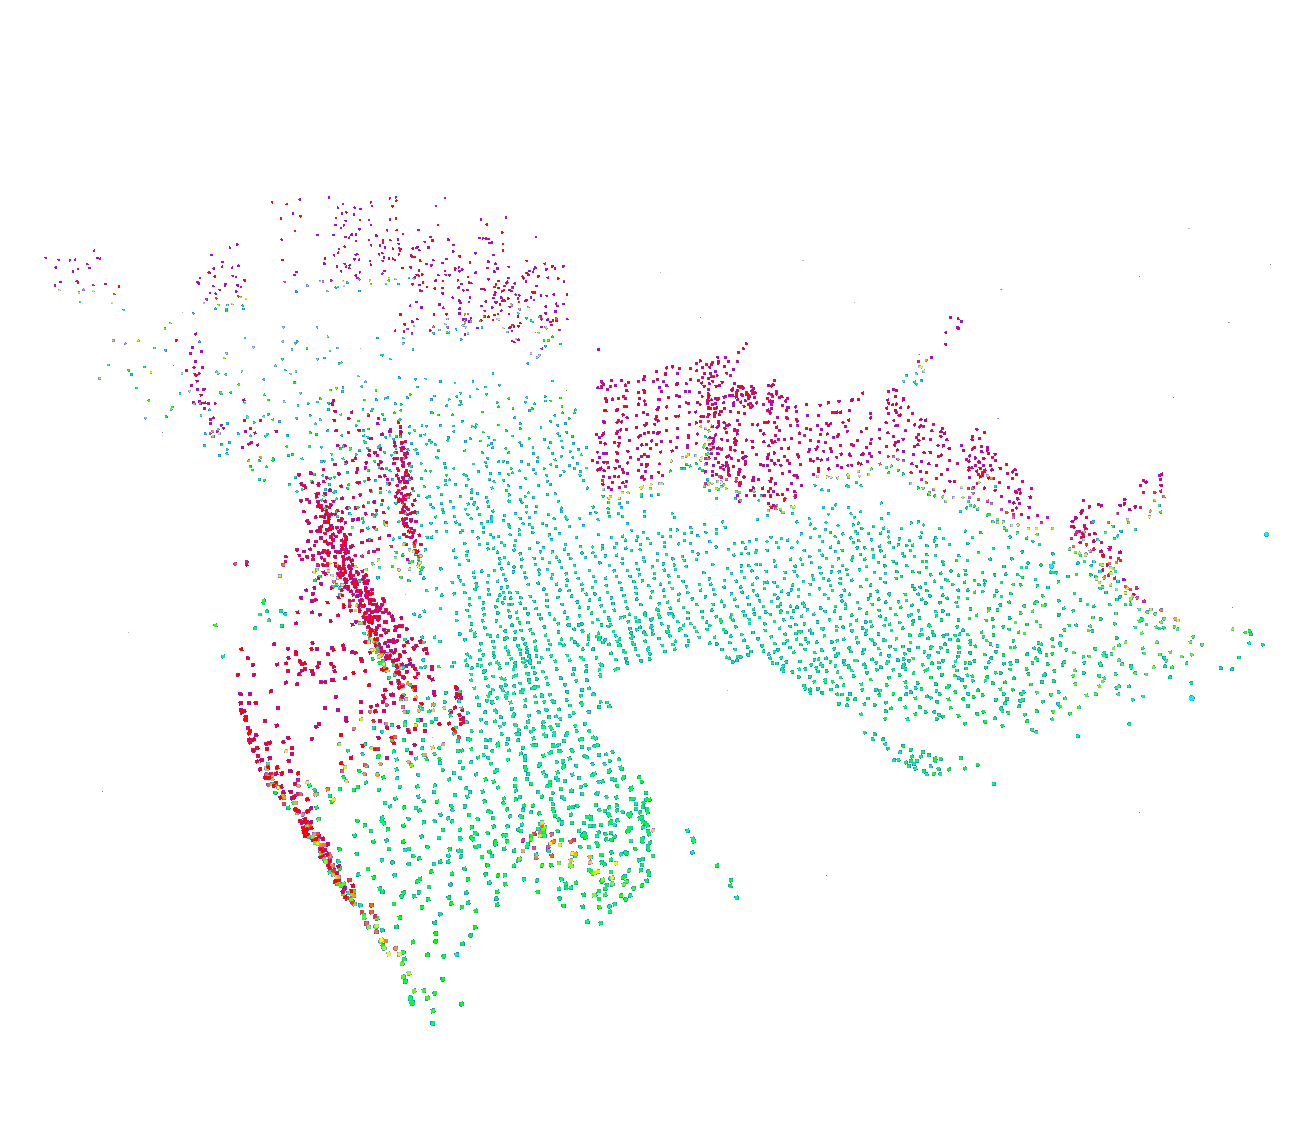
\includegraphics[width=0.45\textwidth]{Images/terrainAnalysis.png}}
            \subfigure[Extended terrain analysis]{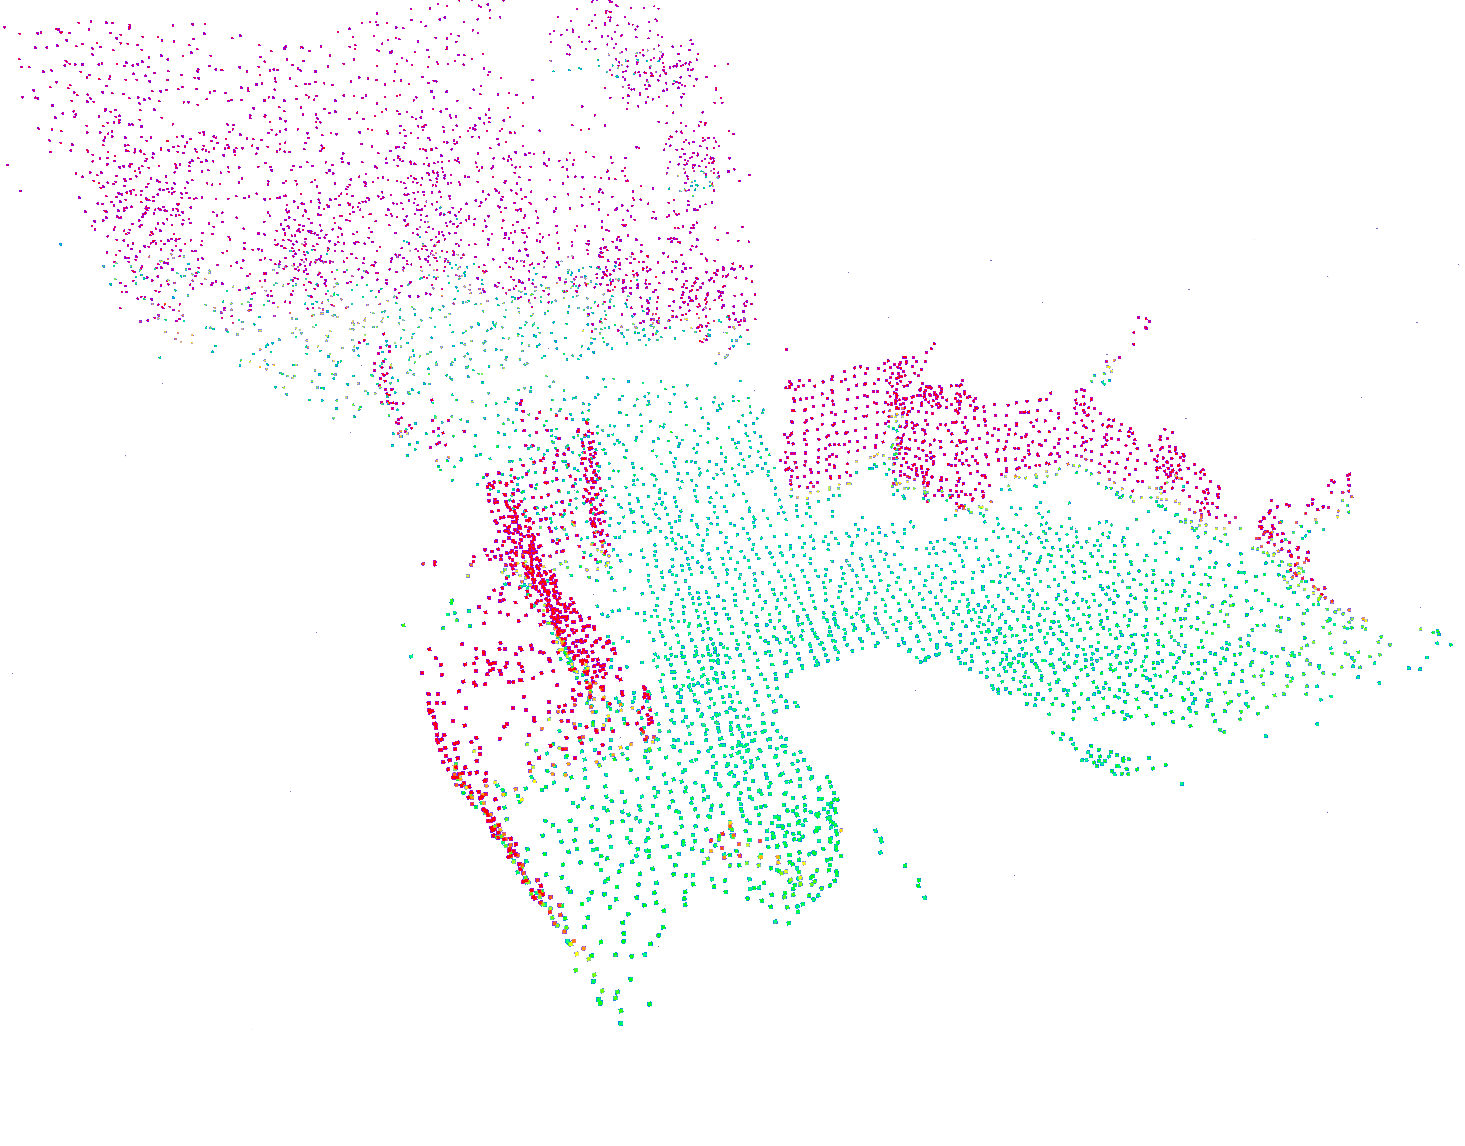
\includegraphics[width=0.45\textwidth]{Images/terrainAnalysisExt2.png}}
            \caption{Comparison of close range and extended range terrain analysis}
            \label{fig:terrain_analysis_comparison}
        \end{figure}

        This terrain analysis paradigm is derived from the works of Ji Shang et al. on fast likelihood-based collision avoidance \cite{zhang2020falco}, as is the local path planning that will be described in section \ref{section:local_path_planning}.

        % TODO add refewrence to this figure
        \begin{figure}[H]
            \centering
            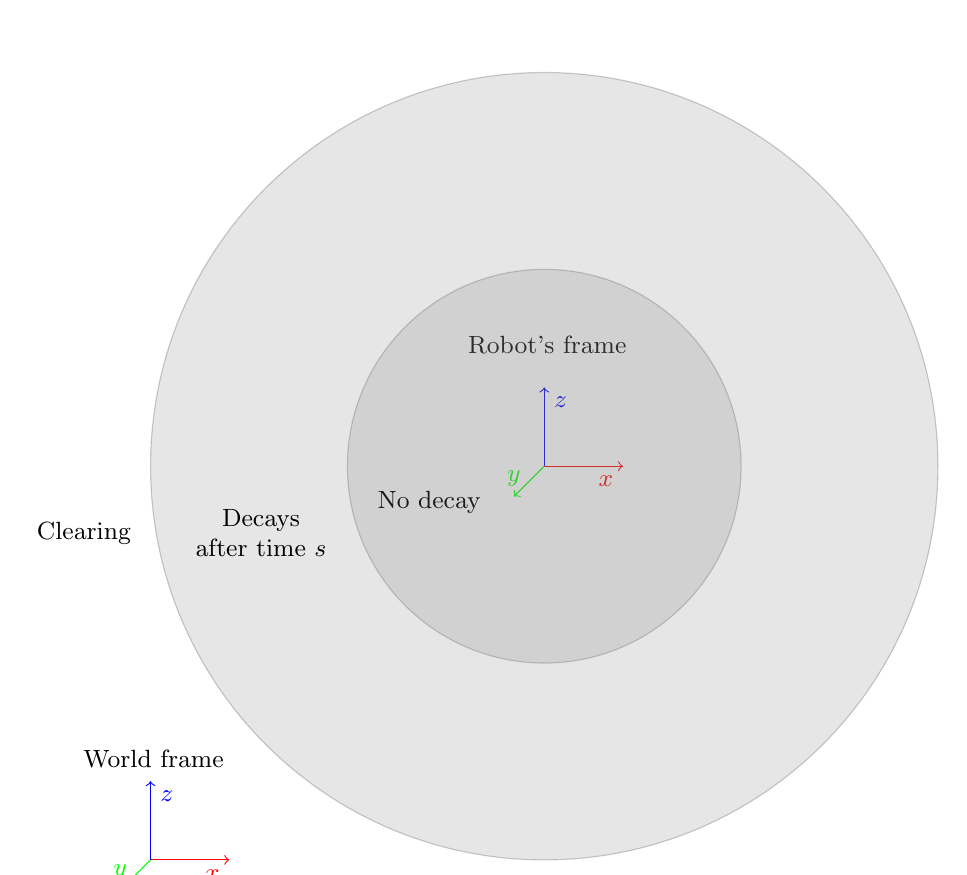
\begin{tikzpicture}[scale=1,font=\small]
                % Robot frame (datum)
                \draw[->,red] (0,0,0) -- (1,0,0) node[anchor=north east]{$x$};
                \draw[->,blue] (0,0,0) -- (0,1,0) node[anchor=north west]{$z$};
                \draw[->,green] (0,0,0) -- (0,0,1) node[anchor=south]{$y$};

                \node at (0.5,2,1.2) {Robot's frame};

                % Spheres
                \draw[fill=gray, opacity=0.2] (0,0,0) circle (2.5cm);
                \node at (-1,0,1.2) {No decay};

                \draw[fill=gray, opacity=0.2] (0,0,0) circle (5cm);
                \node at (-5,0,2.2) {Clearing};
                \node[text width=2cm, align=center] at (-2.75,0,2.2) {Decays after time $s$};

                % World frame (datum)
                \draw[->,red] (-5,-5,0) -- (-4,-5,0) node[anchor=north east]{$x$};
                \draw[->,blue] (-5,-5,0) -- (-5,-4,0) node[anchor=north west]{$z$};
                \draw[->,green] (-5,-5,0) -- (-5,-5,1) node[anchor=south]{$y$};

                \node at (-4.5,-3.25,1.2) {World frame};

            \end{tikzpicture}
            \caption{Decay of the terrain analysis in different zones}
            \label{fig:decay}
        \end{figure}

        The point cloud is split into three zones. In the first zone, the one closest to the robot, the terrain analysis voxels don't get modified but can only get added. This is done to ensure that the robot doesn't forget obstacles when they get closer than the minimum distance the LIDAR can measure. This value was set to $0.1\,\text{m}$ for the quadruped for example.
        The second zone is the zone within which a voxel that has not been hit by the LIDAR for a certain amount of time $s$ get removed. This ensures that the robot doesn't get stopped indefinitely by obstacles that have been removed from the point cloud, like in the case of a human passing by. The third and final zone is the zone within which we clear any terrain voxel present. This is done to ensure that the computation time and memory usage of the terrain analysis doesn't grow indefinitely. This value was set to $8\,\text{m}$ for the regular terrain analysis, and $30\,\text{m}$ for the extended terrain analysis for the quadruped.
        
        Currently, the two terrain analysis are done in parallel, executing the same calculations multiple times. An area of improvement would be to combine both to reduce the total computation time.

    \subsection{Planning}

        The problem of path planning in 2D is a well known problem in robotics and has been solved many times. However, the problem of path planning in 3D is much more complex, and only recently have efficient solutions been found. 

        \subsubsection{2D path planning}
        % Using nav2 as a base and how we convert from a 3D point cloud to a 2D one 
        As a first test of the wheeled and quadruped platform, a simple 2D navigation was put in place to showcase the navigation of the platforms on flat ground. Nav2 \cite{macenski2020marathon2} was used with a simple Smac planner \cite{macenski2024smac} to navigate the platforms. The 3D point cloud was converted to a 2D one by taking only a range of the points relative to the robot's height, the corresponding topic graph can be seen in Figure \ref{fig:pointcloud_to_laserscan}. This was done to showcase the navigation capabilities of the platforms and to test the odometry algorithms. Nav2 was chosen as it is a well known and well documented package that is compatible with every version of ROS2. 
                
        \begin{figure}[H]
            \centering
            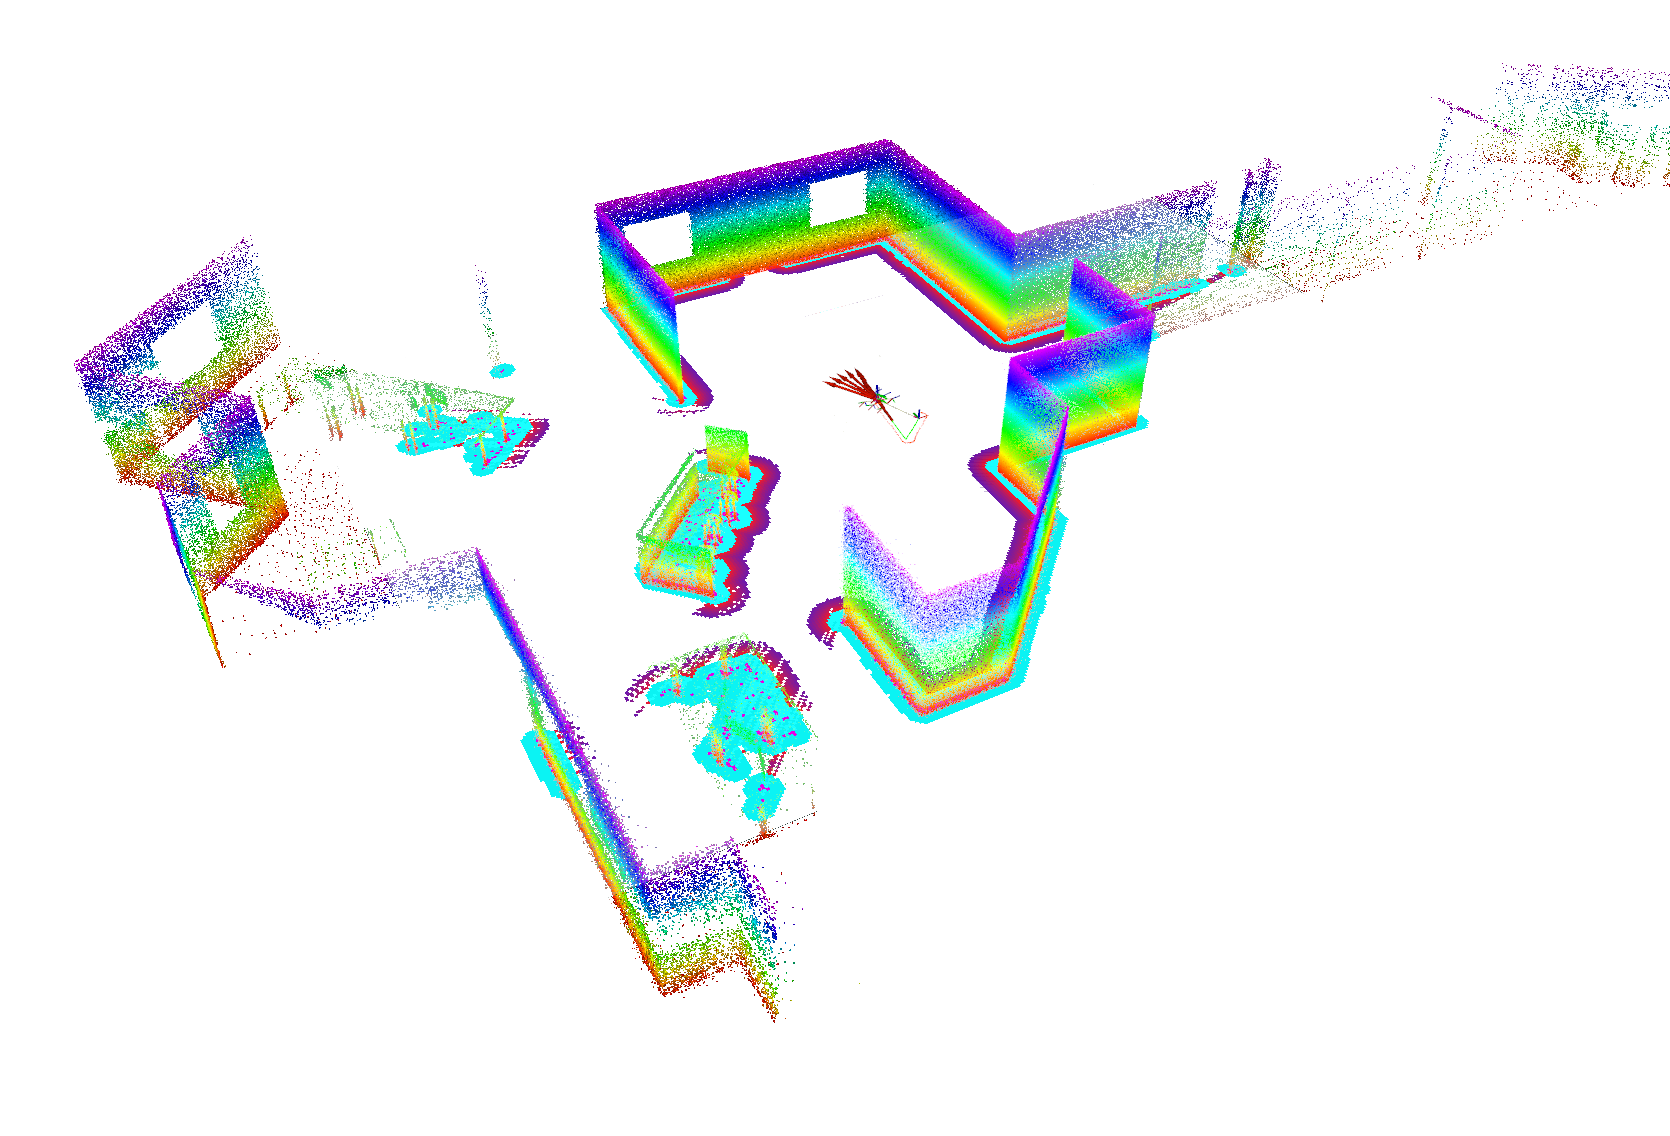
\includegraphics[width=0.8\textwidth]{Images/nav2_costmaps_alpha.png}
            \caption{Nav2 creating multiple costmaps in a simulation, a gradient of colors can be seen around the walls}
            \label{fig:nav2_costmaps}
        \end{figure}
        
        In Figure \ref{fig:nav2_costmaps}, the costmaps, used for navigation, generated by Nav2 can be seen. They represent areas that are free to navigate, areas that are occupied by obstacles, and areas that are unknown. In Figure \ref{fig:nav2_costmaps} they can be seen as purple and blue colored zones around walls and obstacles.  

        \begin{figure}[h]
            \centering
            \resizebox{0.75\textwidth}{!}{%
            
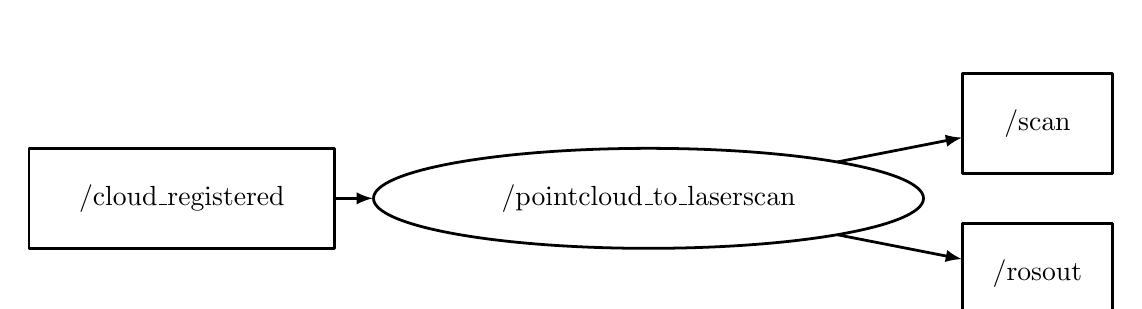
\begin{tikzpicture}[>=latex,line join=bevel,]
  \pgfsetlinewidth{1bp}
%%
\pgfsetcolor{black}
  % Edge: t___cloud_registered -> n___pointcloud_to_laserscan
  \draw [->] (110.35bp,45.0bp) .. controls (111.44bp,45.0bp) and (112.54bp,45.0bp)  .. (123.71bp,45.0bp);
  % Edge: n___pointcloud_to_laserscan -> t___scan
  \draw [->] (290.98bp,58.105bp) .. controls (303.05bp,60.467bp) and (315.21bp,62.845bp)  .. (335.8bp,66.875bp);
  % Edge: n___pointcloud_to_laserscan -> t___rosout
  \draw [->] (290.98bp,31.895bp) .. controls (303.05bp,29.533bp) and (315.21bp,27.155bp)  .. (335.8bp,23.125bp);
  % Node: t___scan
\begin{scope}
  \definecolor{strokecol}{rgb}{0.0,0.0,0.0};
  \pgfsetstrokecolor{strokecol}
  \draw (390.0bp,90.0bp) -- (336.0bp,90.0bp) -- (336.0bp,54.0bp) -- (390.0bp,54.0bp) -- cycle;
  \draw (363.0bp,72.0bp) node {/scan};
\end{scope}
  % Node: t___cloud_registered
\begin{scope}
  \definecolor{strokecol}{rgb}{0.0,0.0,0.0};
  \pgfsetstrokecolor{strokecol}
  \draw (110.0bp,63.0bp) -- (0.0bp,63.0bp) -- (0.0bp,27.0bp) -- (110.0bp,27.0bp) -- cycle;
  \draw (55.0bp,45.0bp) node {/cloud\_registered};
\end{scope}
  % Node: n___pointcloud_to_laserscan
\begin{scope}
  \definecolor{strokecol}{rgb}{0.0,0.0,0.0};
  \pgfsetstrokecolor{strokecol}
  \draw (223.0bp,45.0bp) ellipse (99.0bp and 18.0bp);
  \draw (223.0bp,45.0bp) node {/pointcloud\_to\_laserscan};
\end{scope}
  % Node: t___rosout
\begin{scope}
  \definecolor{strokecol}{rgb}{0.0,0.0,0.0};
  \pgfsetstrokecolor{strokecol}
  \draw (390.0bp,36.0bp) -- (336.0bp,36.0bp) -- (336.0bp,0.0bp) -- (390.0bp,0.0bp) -- cycle;
  \draw (363.0bp,18.0bp) node {/rosout};
\end{scope}
%
\end{tikzpicture}

            }   
            \caption{Conversion from a 3D pointcloud to a 2D scan}
            \label{fig:pointcloud_to_laserscan}
        \end{figure}
        
        
        \subsubsection{3D local path planning}
        \label{section:local_path_planning}

        The local path planning in a 3D environment makes use of the Falco paper \cite{zhang2020falco}. In this paper, a method is proposed where the environment is considered deterministically known within a certain range, usually the range of the LIDAR, and probabilistically known beyond the sensor's range. This contrasts with usual methods that require an online search of a graph that needs updating at every sensor reading. The proposed method by Ji Shang et al. eliminates the need for the online search, favoring a path that maximizes the likelihood to reach the goal, instead of selecting the shortest path like traditional methods.

        %! add reference to figure
        %TODO : add a figure of the local planner paths 
        \begin{figure}[H]
            \centering
            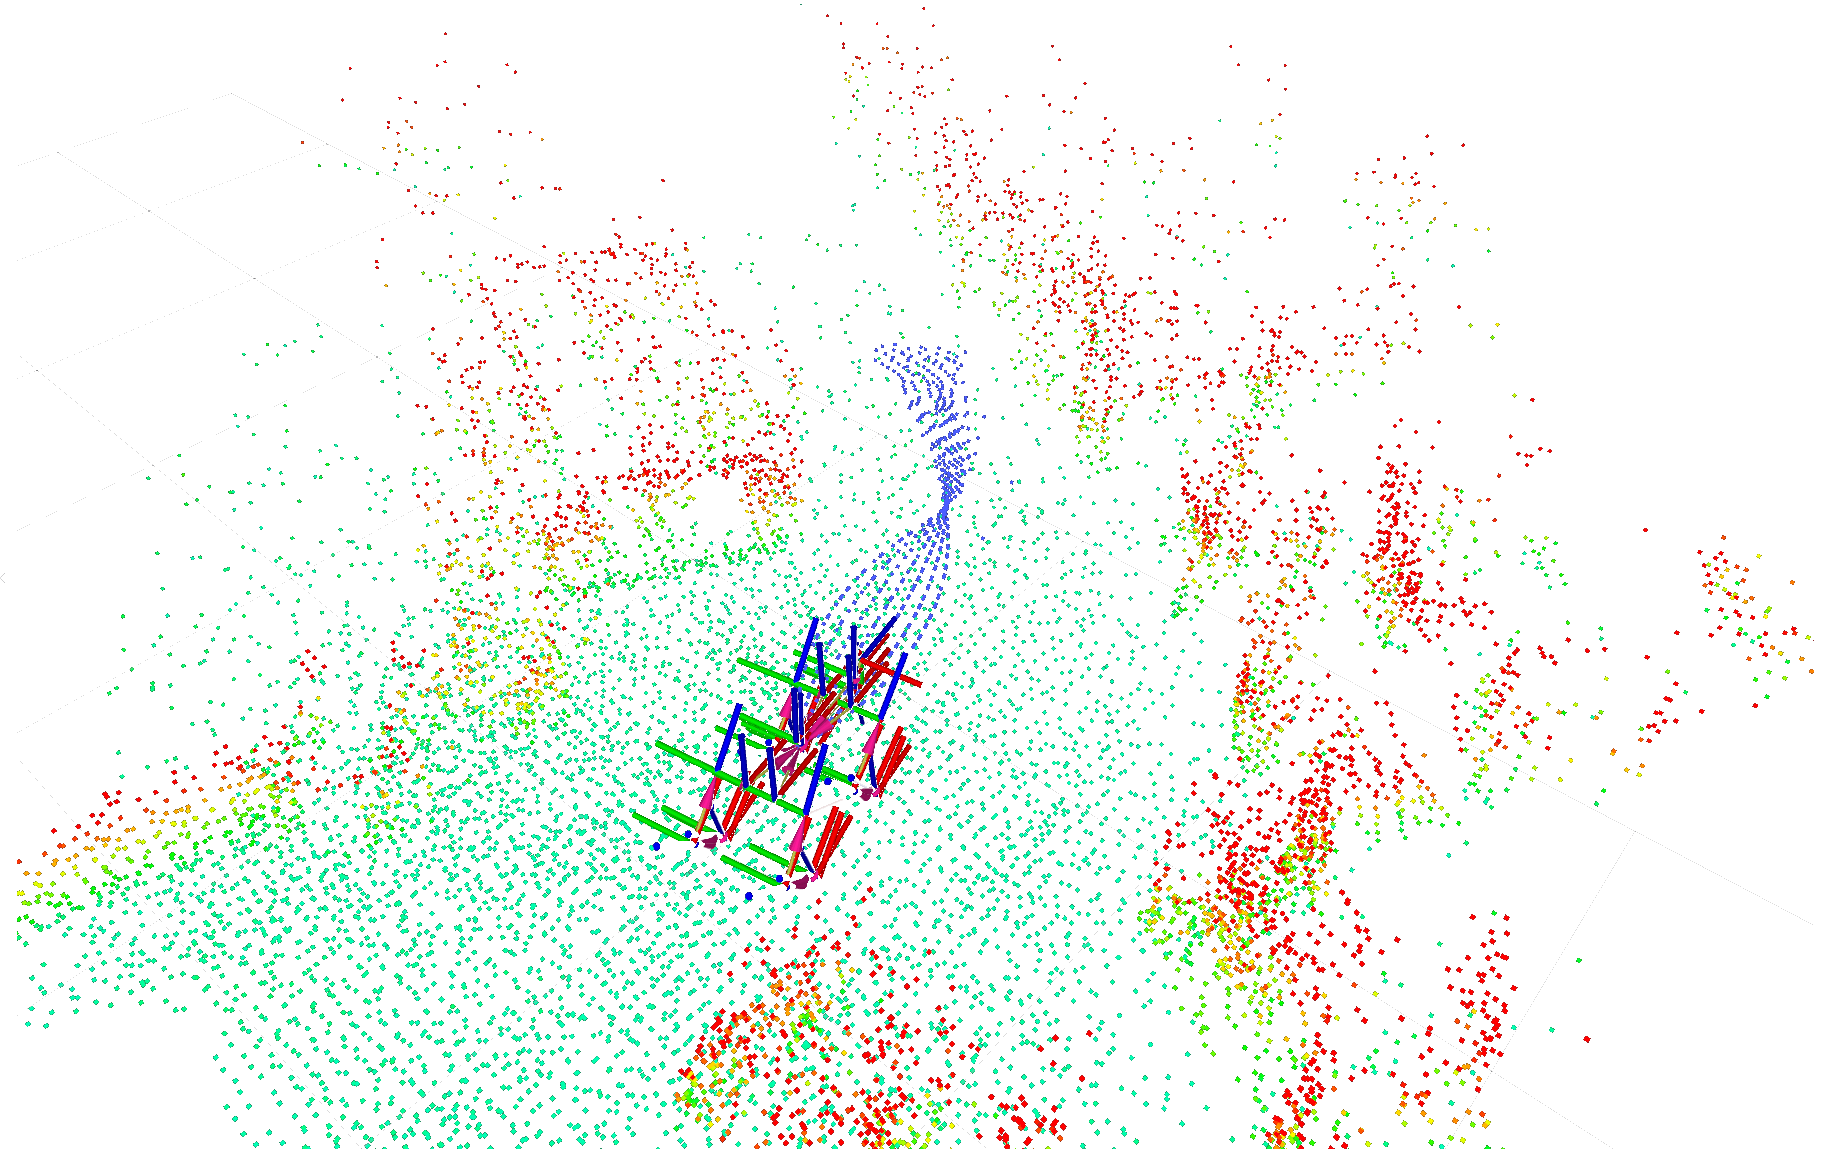
\includegraphics[width=0.75\textwidth]{Images/free_paths.png}
            \caption{Considered paths by the local planner in blue, with terrain analysis pointcloud, the robot is represented as a set of transformed axis}
            \label{fig:local_planner_paths}
        \end{figure}


        The local planner uses the terrain analysis mentioned in section \ref{section:terrain_analysis} to determine the navigable areas. It also subscribes to the odometry, referred to as "/state\_estimation" in Figure \ref{fig:local_planner}, and the registered scan. Its main goal is obtained from the topic "/way\_point" that is generated by the global planner. The local planner then publishes the best path to the topic "/path" that is used by the controller to move the robot, as well as all free paths considered on the topic "/free\_paths". As can be seen in Figure \ref{fig:local_planner}, the local planner also makes sure to only consider paths that are within the exploration boundary if one is defined by subscribing to the topic "/exploration\_boundary". The free paths considered by the local planner can be seen in Figure \ref{fig:local_planner_paths}.

        Setting the correct margin of inflation for the obstacles and the min/max obstacle height for the real robot was a challenge. The margin needed to be large enough to not run into walls and obstacles, but small enough so that the planner would go through tight doorways and passages. 

        To avoid collisions for the quadruped platform, the built-in collision avoidance was also turned on. This resulted in the robot stopping when either the local planner or the collision avoidance detected an obstacle. This was done to ensure the safety of the robot and the environment and proved very reliable in the tests that were done, avoiding collisions with static obstacles, but also with moving obstacles like humans.
        
        \begin{figure}[h]
            \centering
            \resizebox{0.6\textwidth}{!}{%
            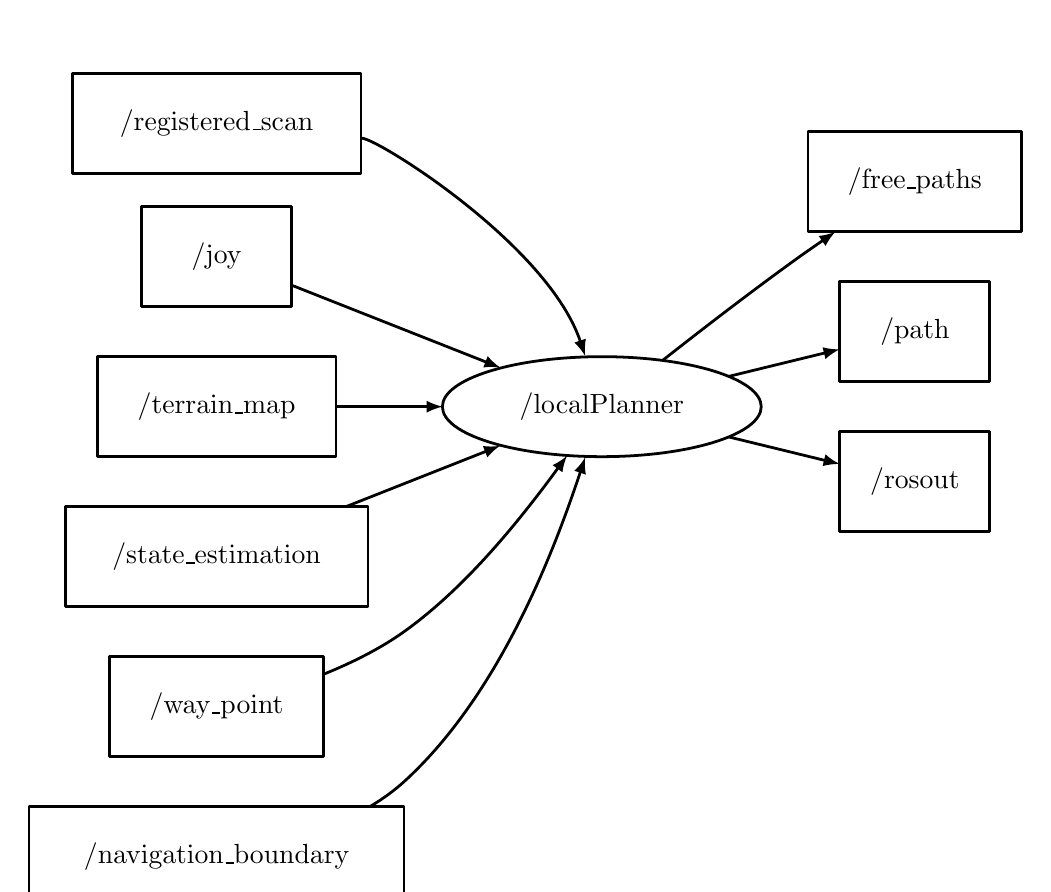
\begin{tikzpicture}[>=latex,line join=bevel,]
  \pgfsetlinewidth{1bp}
%%
\pgfsetcolor{black}
  % Edge: t___added_obstacles -> n___localPlanner
  %\draw [->] (122.25bp,433.02bp) .. controls (126.91bp,430.16bp) and (131.27bp,426.85bp)  .. (135.0bp,423.0bp) .. controls (178.86bp,377.8bp) and (195.74bp,302.78bp)  .. (203.31bp,252.17bp);
  % Edge: n___localPlanner -> t___free_paths
  \draw [->] (228.11bp,250.68bp) .. controls (241.92bp,261.55bp) and (260.52bp,275.91bp)  .. (277.39bp,288.0bp) .. controls (278.81bp,289.02bp) and (280.26bp,290.04bp)  .. (290.27bp,296.95bp);
  % Edge: n___localPlanner -> t___path
  \draw [->] (251.9bp,244.9bp) .. controls (261.86bp,247.33bp) and (272.29bp,249.88bp)  .. (291.82bp,254.64bp);
  % Edge: n___localPlanner -> t___rosout
  \draw [->] (251.9bp,223.1bp) .. controls (261.86bp,220.67bp) and (272.29bp,218.12bp)  .. (291.82bp,213.36bp);
  % Edge: t___registered_scan -> n___localPlanner
  \draw [->] (119.77bp,330.65bp) .. controls (125.26bp,330.64bp)  and (186.98bp,292.29bp)  .. (200.19bp,252.26bp);
  % Edge: t___check_obstacle -> n___localPlanner
  %\draw [->] (119.23bp,324.39bp) .. controls (124.76bp,321.61bp) and (130.14bp,318.48bp)  .. (135.0bp,315.0bp) .. controls (155.87bp,300.06bp) and (174.64bp,277.7bp)  .. (193.67bp,251.65bp);
  % Edge: t___joy -> n___localPlanner
  \draw [->] (94.533bp,277.72bp) .. controls (113.09bp,270.39bp) and (138.51bp,260.34bp)  .. (169.71bp,248.02bp);
  % Edge: t___terrain_map -> n___localPlanner
  \draw [->] (110.63bp,234.0bp) .. controls (119.5bp,234.0bp) and (129.07bp,234.0bp)  .. (148.87bp,234.0bp);
  % Edge: t___state_estimation -> n___localPlanner
  \draw [->] (114.4bp,198.13bp) .. controls (129.16bp,203.96bp) and (145.49bp,210.41bp)  .. (169.58bp,219.93bp);
  % Edge: t___way_point -> n___localPlanner
  \draw [->] (106.35bp,137.8bp) .. controls (116.16bp,141.79bp) and (126.39bp,146.84bp)  .. (135.0bp,153.0bp) .. controls (155.87bp,167.94bp) and (174.64bp,190.3bp)  .. (193.67bp,216.35bp);
  % Edge: t___navigation_boundary -> n___localPlanner
  \draw [->] (122.77bp,90.063bp) .. controls (127.16bp,92.679bp) and (131.31bp,95.645bp)  .. (135.0bp,99.0bp) .. controls (167.15bp,128.27bp) and (186.98bp,175.71bp)  .. (200.19bp,215.74bp);
  % Edge: t___speed -> n___localPlanner
  %\draw [->] (94.726bp,23.288bp) .. controls (108.3bp,27.23bp) and (124.24bp,33.912bp)  .. (135.0bp,45.0bp) .. controls (178.86bp,90.196bp) and (195.74bp,165.22bp)  .. (203.31bp,215.83bp);
  % Node: t___added_obstacles
% \begin{scope}
%   \definecolor{strokecol}{rgb}{0.0,0.0,0.0};
%   \pgfsetstrokecolor{strokecol}
%   \draw (122.0bp,468.0bp) -- (13.0bp,468.0bp) -- (13.0bp,432.0bp) -- (122.0bp,432.0bp) -- cycle;
%   \draw (67.5bp,450.0bp) node {/added\_obstacles};
% \end{scope}
  % Node: n___localPlanner
\begin{scope}
  \definecolor{strokecol}{rgb}{0.0,0.0,0.0};
  \pgfsetstrokecolor{strokecol}
  \draw (206.19bp,234.0bp) ellipse (57.39bp and 18.0bp);
  \draw (206.19bp,234.0bp) node {/localPlanner};
\end{scope}
  % Node: t___free_paths
\begin{scope}
  \definecolor{strokecol}{rgb}{0.0,0.0,0.0};
  \pgfsetstrokecolor{strokecol}
  \draw (357.39bp,333.0bp) -- (280.39bp,333.0bp) -- (280.39bp,297.0bp) -- (357.39bp,297.0bp) -- cycle;
  \draw (318.89bp,315.0bp) node {/free\_paths};
\end{scope}
  % Node: t___path
\begin{scope}
  \definecolor{strokecol}{rgb}{0.0,0.0,0.0};
  \pgfsetstrokecolor{strokecol}
  \draw (345.89bp,279.0bp) -- (291.89bp,279.0bp) -- (291.89bp,243.0bp) -- (345.89bp,243.0bp) -- cycle;
  \draw (318.89bp,261.0bp) node {/path};
\end{scope}
  % Node: t___rosout
\begin{scope}
  \definecolor{strokecol}{rgb}{0.0,0.0,0.0};
  \pgfsetstrokecolor{strokecol}
  \draw (345.89bp,225.0bp) -- (291.89bp,225.0bp) -- (291.89bp,189.0bp) -- (345.89bp,189.0bp) -- cycle;
  \draw (318.89bp,207.0bp) node {/rosout};
\end{scope}
  % Node: t___registered_scan
\begin{scope}
  \definecolor{strokecol}{rgb}{0.0,0.0,0.0};
  \pgfsetstrokecolor{strokecol}
  \draw (119.5bp,354.0bp) -- (15.5bp,354.0bp) -- (15.5bp,318.0bp) -- (119.5bp,318.0bp) -- cycle;
  \draw (67.5bp,336.0bp) node {/registered\_scan};
\end{scope}
  % Node: t___check_obstacle
%\begin{scope}
%  \definecolor{strokecol}{rgb}{0.0,0.0,0.0};
%  \pgfsetstrokecolor{strokecol}
%  \draw (119.0bp,360.0bp) -- (16.0bp,360.0bp) -- (16.0bp,324.0bp) -- (119.0bp,324.0bp) -- cycle;
%  \draw (67.5bp,342.0bp) node {/check\_obstacle};
%\end{scope}
  % Node: t___joy
\begin{scope}
  \definecolor{strokecol}{rgb}{0.0,0.0,0.0};
  \pgfsetstrokecolor{strokecol}
  \draw (94.5bp,306.0bp) -- (40.5bp,306.0bp) -- (40.5bp,270.0bp) -- (94.5bp,270.0bp) -- cycle;
  \draw (67.5bp,288.0bp) node {/joy};
\end{scope}
  % Node: t___terrain_map
\begin{scope}
  \definecolor{strokecol}{rgb}{0.0,0.0,0.0};
  \pgfsetstrokecolor{strokecol}
  \draw (110.5bp,252.0bp) -- (24.5bp,252.0bp) -- (24.5bp,216.0bp) -- (110.5bp,216.0bp) -- cycle;
  \draw (67.5bp,234.0bp) node {/terrain\_map};
\end{scope}
  % Node: t___state_estimation
\begin{scope}
  \definecolor{strokecol}{rgb}{0.0,0.0,0.0};
  \pgfsetstrokecolor{strokecol}
  \draw (122.0bp,198.0bp) -- (13.0bp,198.0bp) -- (13.0bp,162.0bp) -- (122.0bp,162.0bp) -- cycle;
  \draw (67.5bp,180.0bp) node {/state\_estimation};
\end{scope}
  % Node: t___way_point
\begin{scope}
  \definecolor{strokecol}{rgb}{0.0,0.0,0.0};
  \pgfsetstrokecolor{strokecol}
  \draw (106.0bp,144.0bp) -- (29.0bp,144.0bp) -- (29.0bp,108.0bp) -- (106.0bp,108.0bp) -- cycle;
  \draw (67.5bp,126.0bp) node {/way\_point};
\end{scope}
  % Node: t___navigation_boundary
\begin{scope}
  \definecolor{strokecol}{rgb}{0.0,0.0,0.0};
  \pgfsetstrokecolor{strokecol}
  \draw (135.0bp,90.0bp) -- (0.0bp,90.0bp) -- (0.0bp,54.0bp) -- (135.0bp,54.0bp) -- cycle;
  \draw (67.5bp,72.0bp) node {/navigation\_boundary};
\end{scope}
  % Node: t___speed
%\begin{scope}
%  \definecolor{strokecol}{rgb}{0.0,0.0,0.0};
%  \pgfsetstrokecolor{strokecol}
%  \draw (94.5bp,36.0bp) -- (40.5bp,36.0bp) -- (40.5bp,0.0bp) -- (94.5bp,0.0bp) -- cycle;
%  \draw (67.5bp,18.0bp) node {/speed};
%\end{scope}
%
\end{tikzpicture}

            }   
            \caption{localPlanner subscriptions and publications}
            \label{fig:local_planner}
        \end{figure}
        
        % \begin{figure}[h!]
        %     \centering
        %     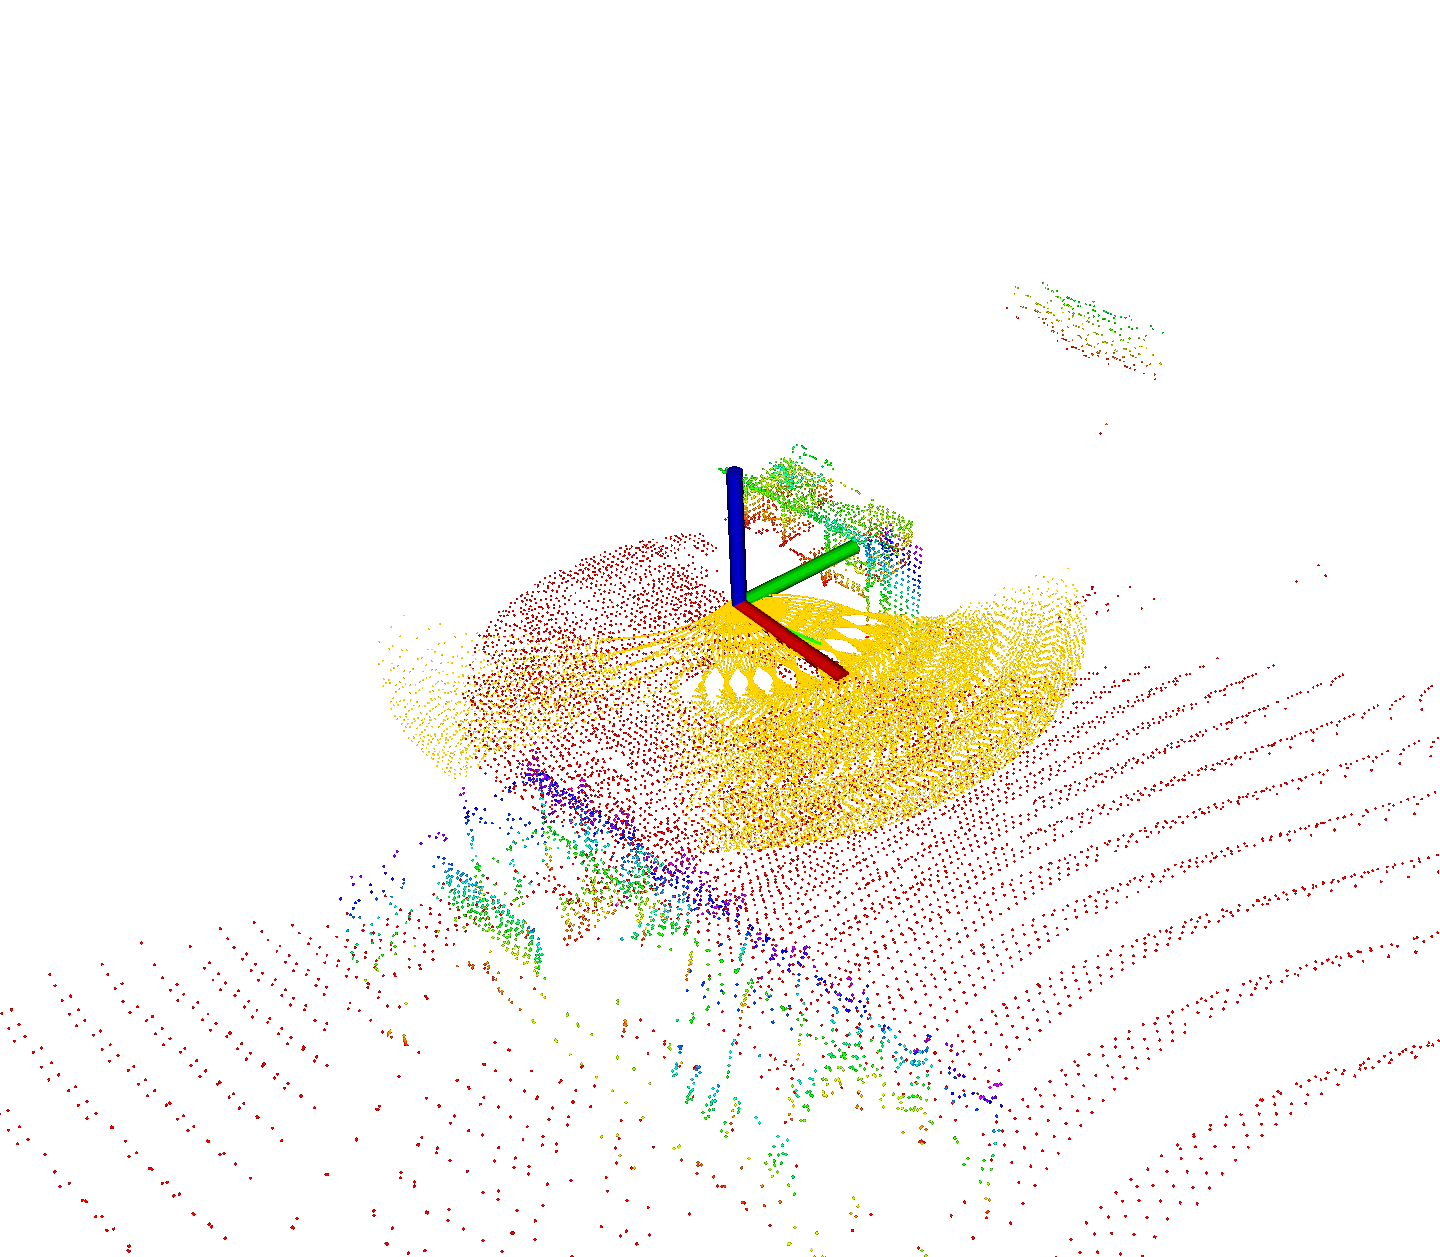
\includegraphics[width=0.65\textwidth]{Images/localPlannerSimCropped.png}
        %     \caption{Local planner in simulation, the yellow points are the considered paths, the other points are from the terrain analysis. The robot is represented as a set of axis}
        %     \label{fig:local_planner_sim}
        % \end{figure}

        % TODO also add the path following node explaination
        
        
        \subsubsection{Comparison of 3D Planning Algorithms}

        3D path planning algorithms can be divided in multiple categories, each tailored to specific world representation, with distinct strengths and limitations. Sampling-based algorithms, such as Rapidly-Exploring Random Trees \cite{lavalle1998rapidly} (RRT) and Probabilistic Roadmaps\cite{kavraki1996probabilistic} (PRM), are particularly effective in navigating complex environments. These algorithms are highly flexible and incrementally construct paths, making them suitable for real-time applications. However, they can suffer from inefficiencies caused by random sampling, which may result in suboptimal paths in real world scenarios. Advanced versions like RRT* \cite{islam2012rrt} enhance the optimality of the generated paths, while adaptive PRM methods reduce computational demands in dynamic environments.
        
        Node-based algorithms, including A* and its derivatives, are renowned for their proven optimality under specific conditions. These algorithms operate by exploring nodes in a predefined graph and are highly effective in dynamic environments. Variants such as Theta* improve upon A* by generating paths with realistic shapes better suited for real-world terrains. However, their reliance on dense grids for 3D environments can lead to significant computational overhead, especially in cluttered or expansive workspaces.
        
        Bioinspired algorithms, such as Ant Colony Optimization (ACO) and Particle Swarm Optimization (PSO), draw inspiration from natural phenomena to address complex, unstructured environments. These methods excel in solving NP-hard problems and can adapt well to challenging scenarios. Despite their robustness, they often require extensive computational resources and careful parameter tuning to achieve optimal results.
        
        Mathematical model-based algorithms provide rigorously defined solutions by incorporating kinodynamic constraints into their formulations. While these methods offer precise paths and control mechanisms, their dependence on accurate environmental models and high computational costs can limit their practicality in real-time applications.
        
        Finally, hybrid or multifusion algorithms combine elements from multiple approaches, such as integrating A* with RRT*, to leverage the complementary strengths of individual methods. These hybrid strategies excel in balancing adaptability and computational efficiency but may introduce additional complexity in their implementation and fine-tuning.
        
        The choice of algorithm depends largely on the specific requirements of the task, including computational efficiency, environmental adaptability, and the precision needed for the robotic application.
        

        

    \subsection{Exploration}

        In the field of robotics, exploration is the conception of trajectories that provide more coverage of the environment for the sensors. It is inherently linked to the mapping and path planning processes, as exploration requires the robot to know where it is and where it can go.  
        
        \subsubsection{Metrics for exploration}
        % show how we calculate the exploration rate using the tools provided in the TARE planner
        % explain the need for a pre-recorded pointcloud of the area we wish to explore
        
        Exploration efficiency can be quantified by the exploration rate, which measures the amount of new information gathered by a robot over a period of time. This metric can be defined as either the surface area or volume of the environment covered by the aggregation of all sensor readings over time. The exploration rate is crucial for optimizing the efficiency of robotic exploration missions, as it directly impacts the speed and thus the time required to fully map an environment. 

        Another metric that is important for robotics exploration is the final area or volume covered by the robot. This demonstrates how thorough the exploration was, and can be used to compare different exploration strategies.

        Finally, as the exploration algorithm is executed on an embedded computer, the computational cost of the algorithm is also an important metric to consider. 

        The problem of exploration remains a challenging and open one, as described in \cite{lluvia2021active}. But advancements in reinforcement learning approaches to the problem \cite{garaffa2021reinforcement} have helped improve the efficiency in certain scenarios but still lack the robustness of traditional methods.

        \subsubsection{TARE planner}
        % go in details about the process that the TARE-planner uses to explore and the motivations for the original creation of this planner (darpa sub teranean chaleneg)

        TARE \cite{tare}, is a hierarchical framework for exploring unknown 3D environment. This planner was designed for Carnegie Mellon University's participation at the 2021 DARPA subterranean challenge \cite{darpa_subterranean_challenge}. In Figure \ref{fig:tare_darpa_exploration}, the exploration of one of DARPA's environments  can be seen explored by tare planner. The planner doesn't use any prerecorded point cloud for exploration, but uses a viewpoint candidate method for exploration. The planner is able to explore large environments by building a reduced local path, while maintaining a coarse global path.

        Viewpoint candidates are generated by the planner within the local planning horizon (see Figure \ref{fig:tare_local_global}), and on valid positions of the terrain map. Each candidate is then evaluated for the amount of information it would bring to the map. This is done by evaluating the uncovered surface of the map, and evaluating the amount of those areas the viewpoint candidate would cover from the LIDAR's perspective.  

        This method also implements a hierarchical exploration strategy where the entire exploration path is considered, rather than greedily maximizing the exploration rate. In contrasts to other methods such as Motion primitive-Based exploration with path-Planner (MBP) \cite{dharmadhikari2020motion} or the Next Best View Planner (NBVP) \cite{bircher2016receding}, this method is able to explore large environments with a high exploration rate.


        \begin{figure}[H]
            \centering
            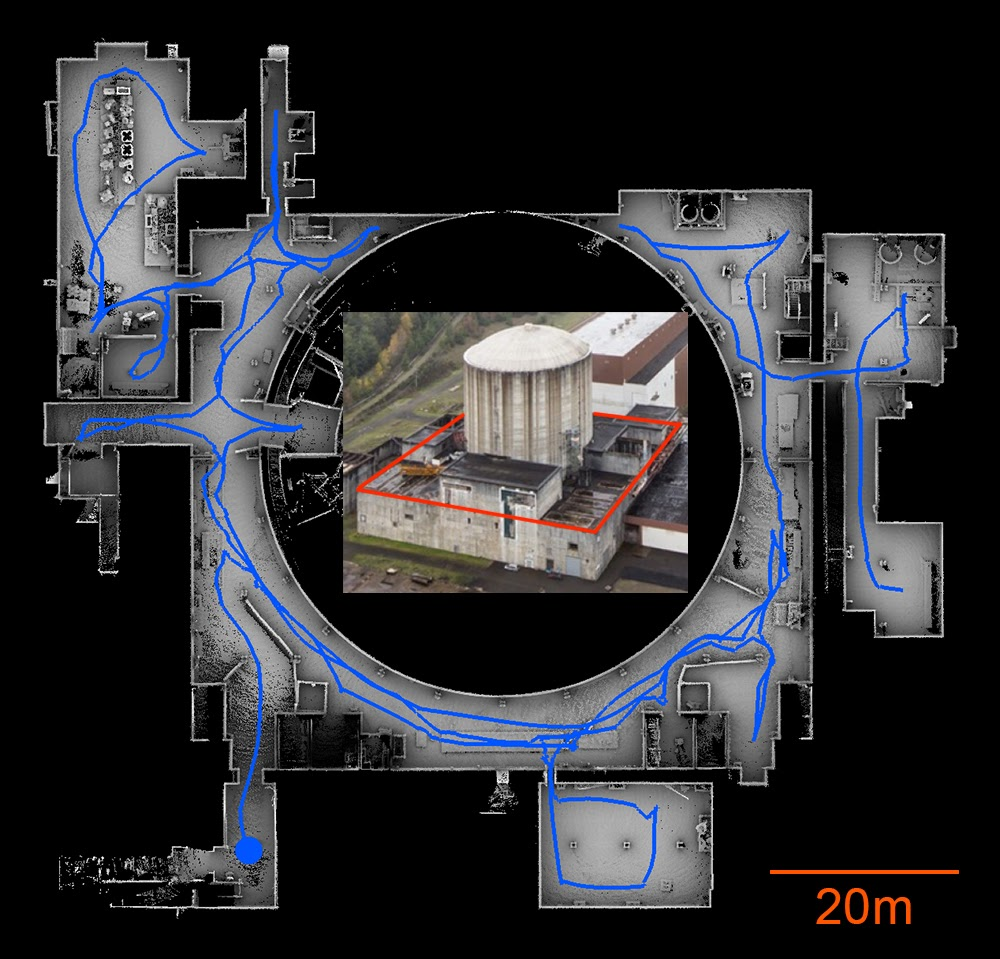
\includegraphics[width=0.7\textwidth]{Images/tare_darpa_exploration.jpg}
            \caption{TARE planner exploration during DARPA SubT challenge, from \cite{tare}}
            \label{fig:tare_darpa_exploration}
        \end{figure}

        \begin{figure}[H]
            \centering
            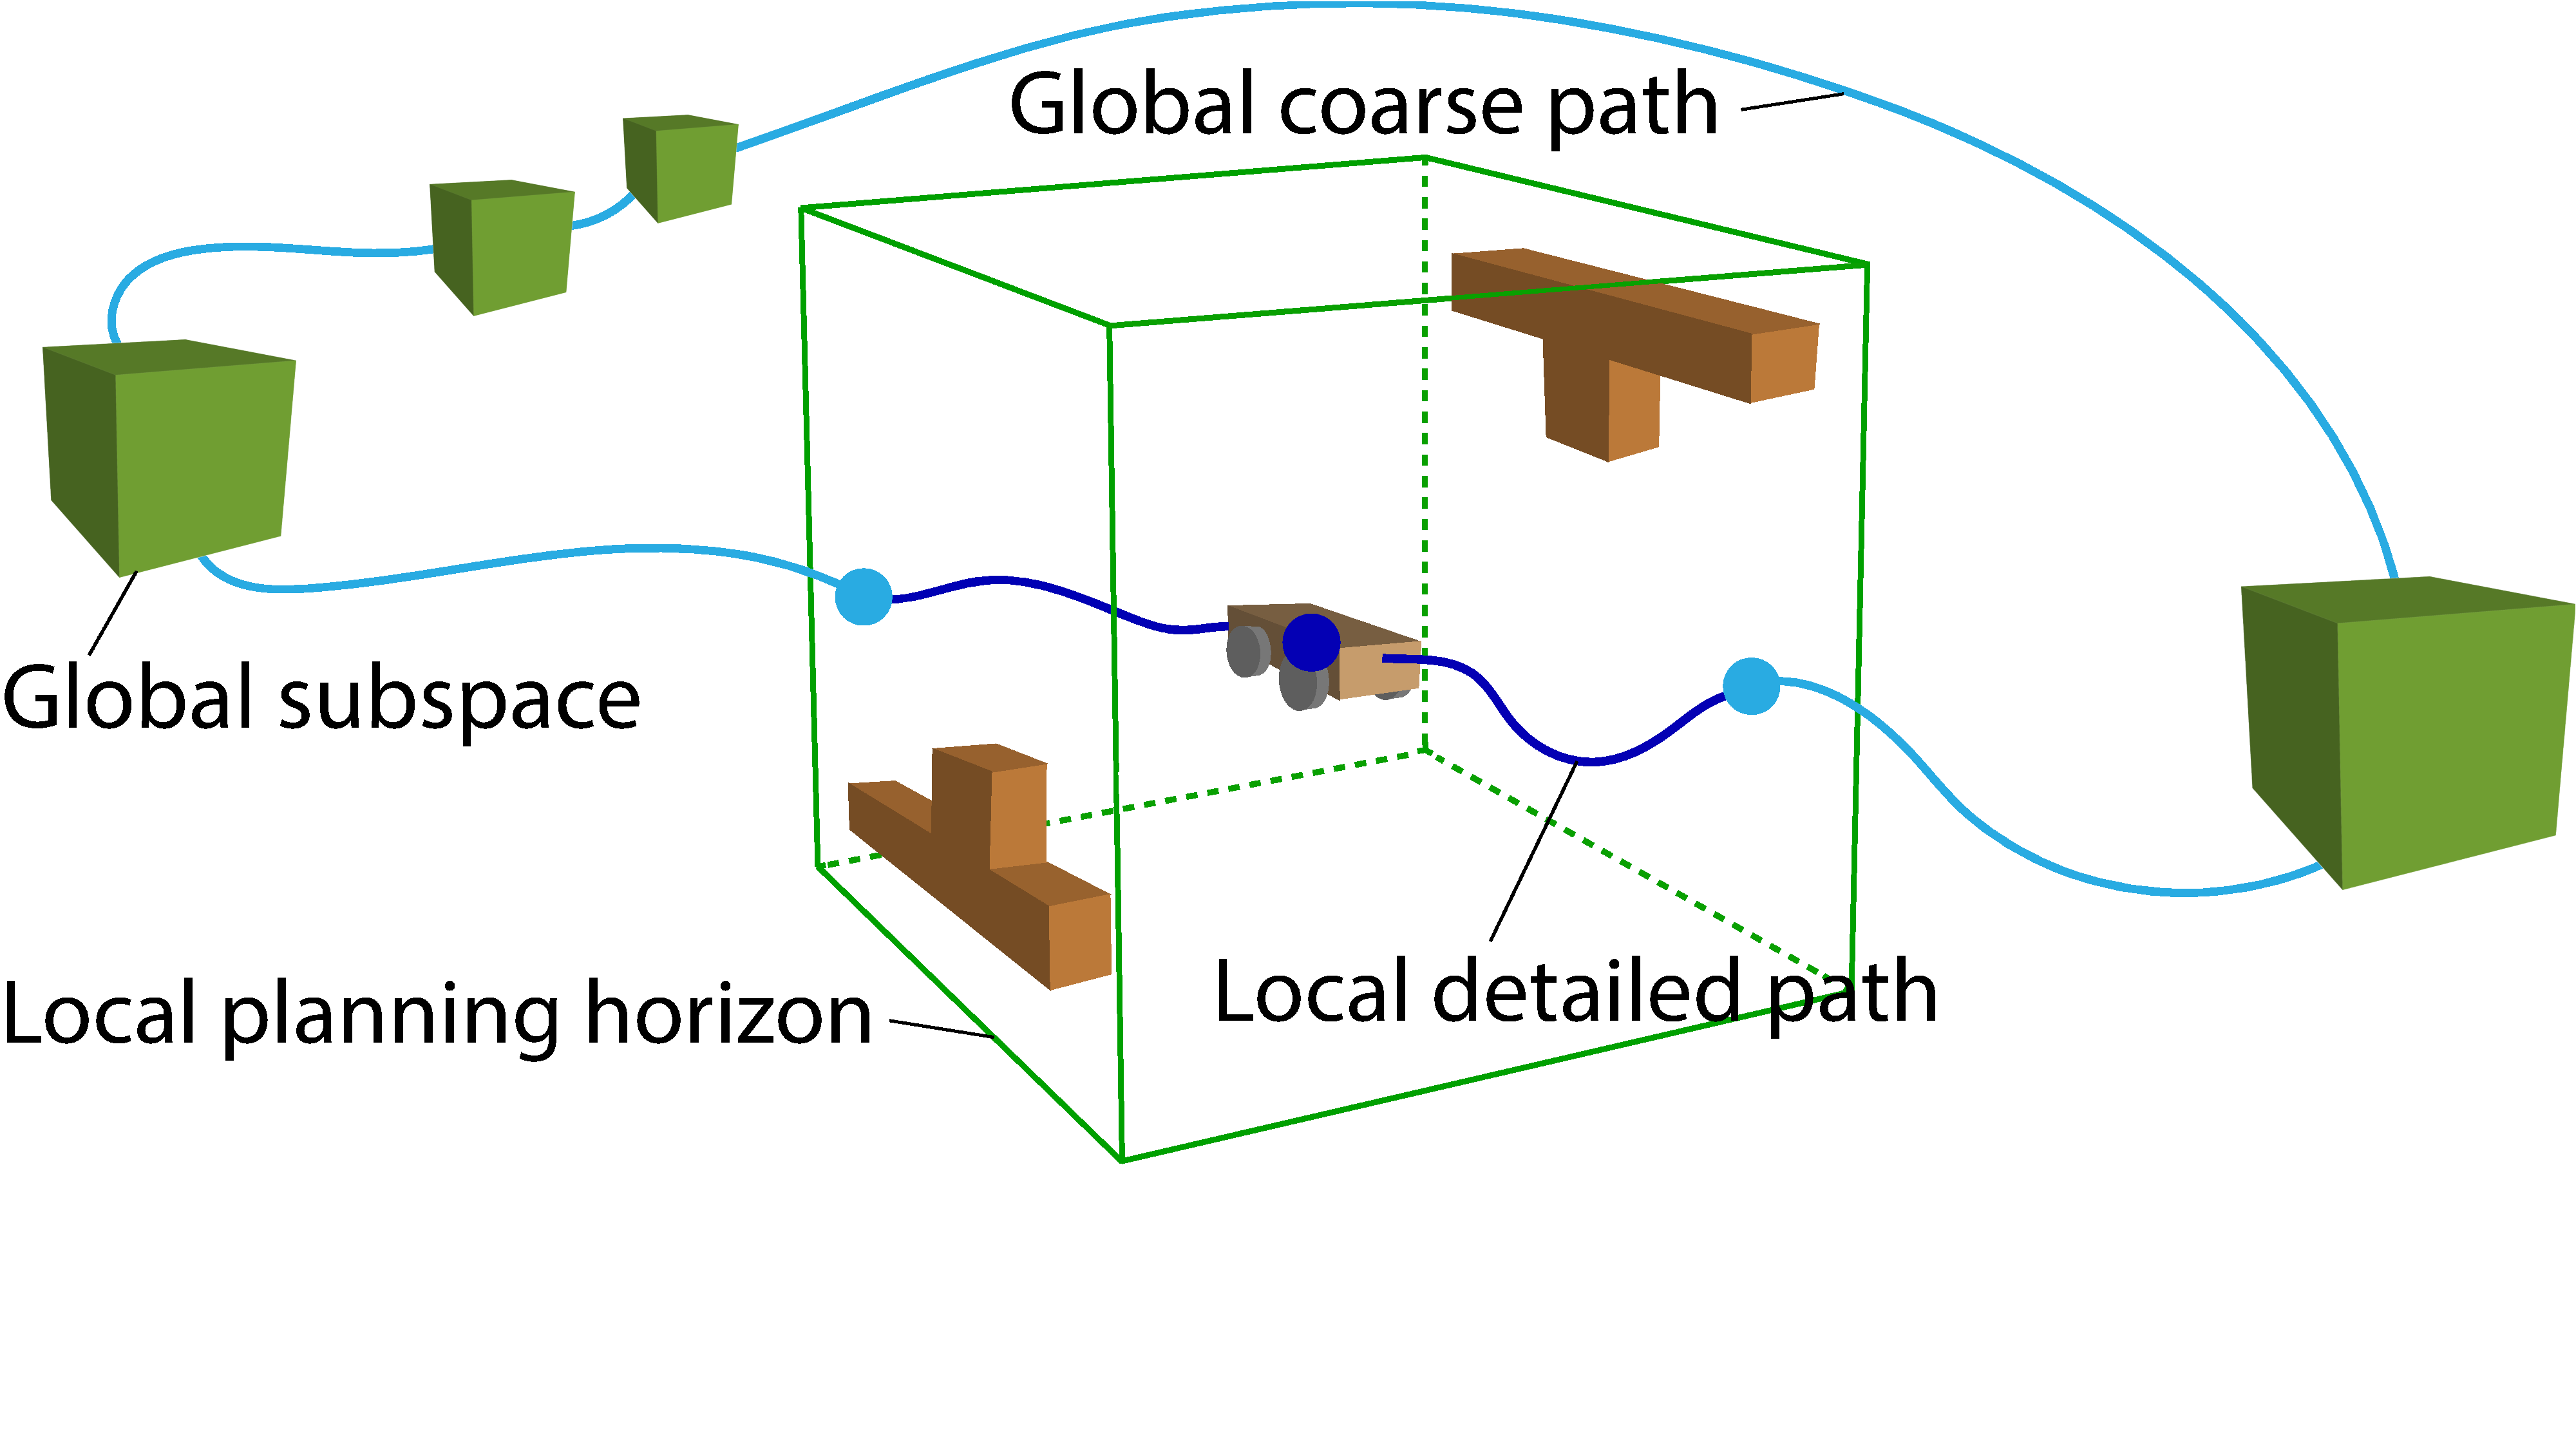
\includegraphics[width=0.7\textwidth]{Images/tare.pdf}
            \caption{Local and global paths of the TARE planner, a dense map is conserved only for the local planning horizon, while a sparse map is kept for the global planning, from \cite{tare}}
            \label{fig:tare_local_global}
        \end{figure}


        A test was performed with the TARE planner in a real environment to showcase the exploration capabilities of the planner. The environment chosen is the ground floor of the Alumni Hall at IIT that features a concrete testing lab, a machine shop, a classroom, and two entryways. In Figure \ref{fig:tare_iit_exploration}, the exploration of the Alumni Hall can be seen. The planner was able to explore most of the environment in a less than 10 minutes. It however struggled to go through tight passages, like certain doorways, but did not require any manual interventions. The resulting map captured by the LIDAR of the GO2 can be seen in Figure \ref{fig:tare_iit_map}.


        \begin{figure}[H]
            \centering
            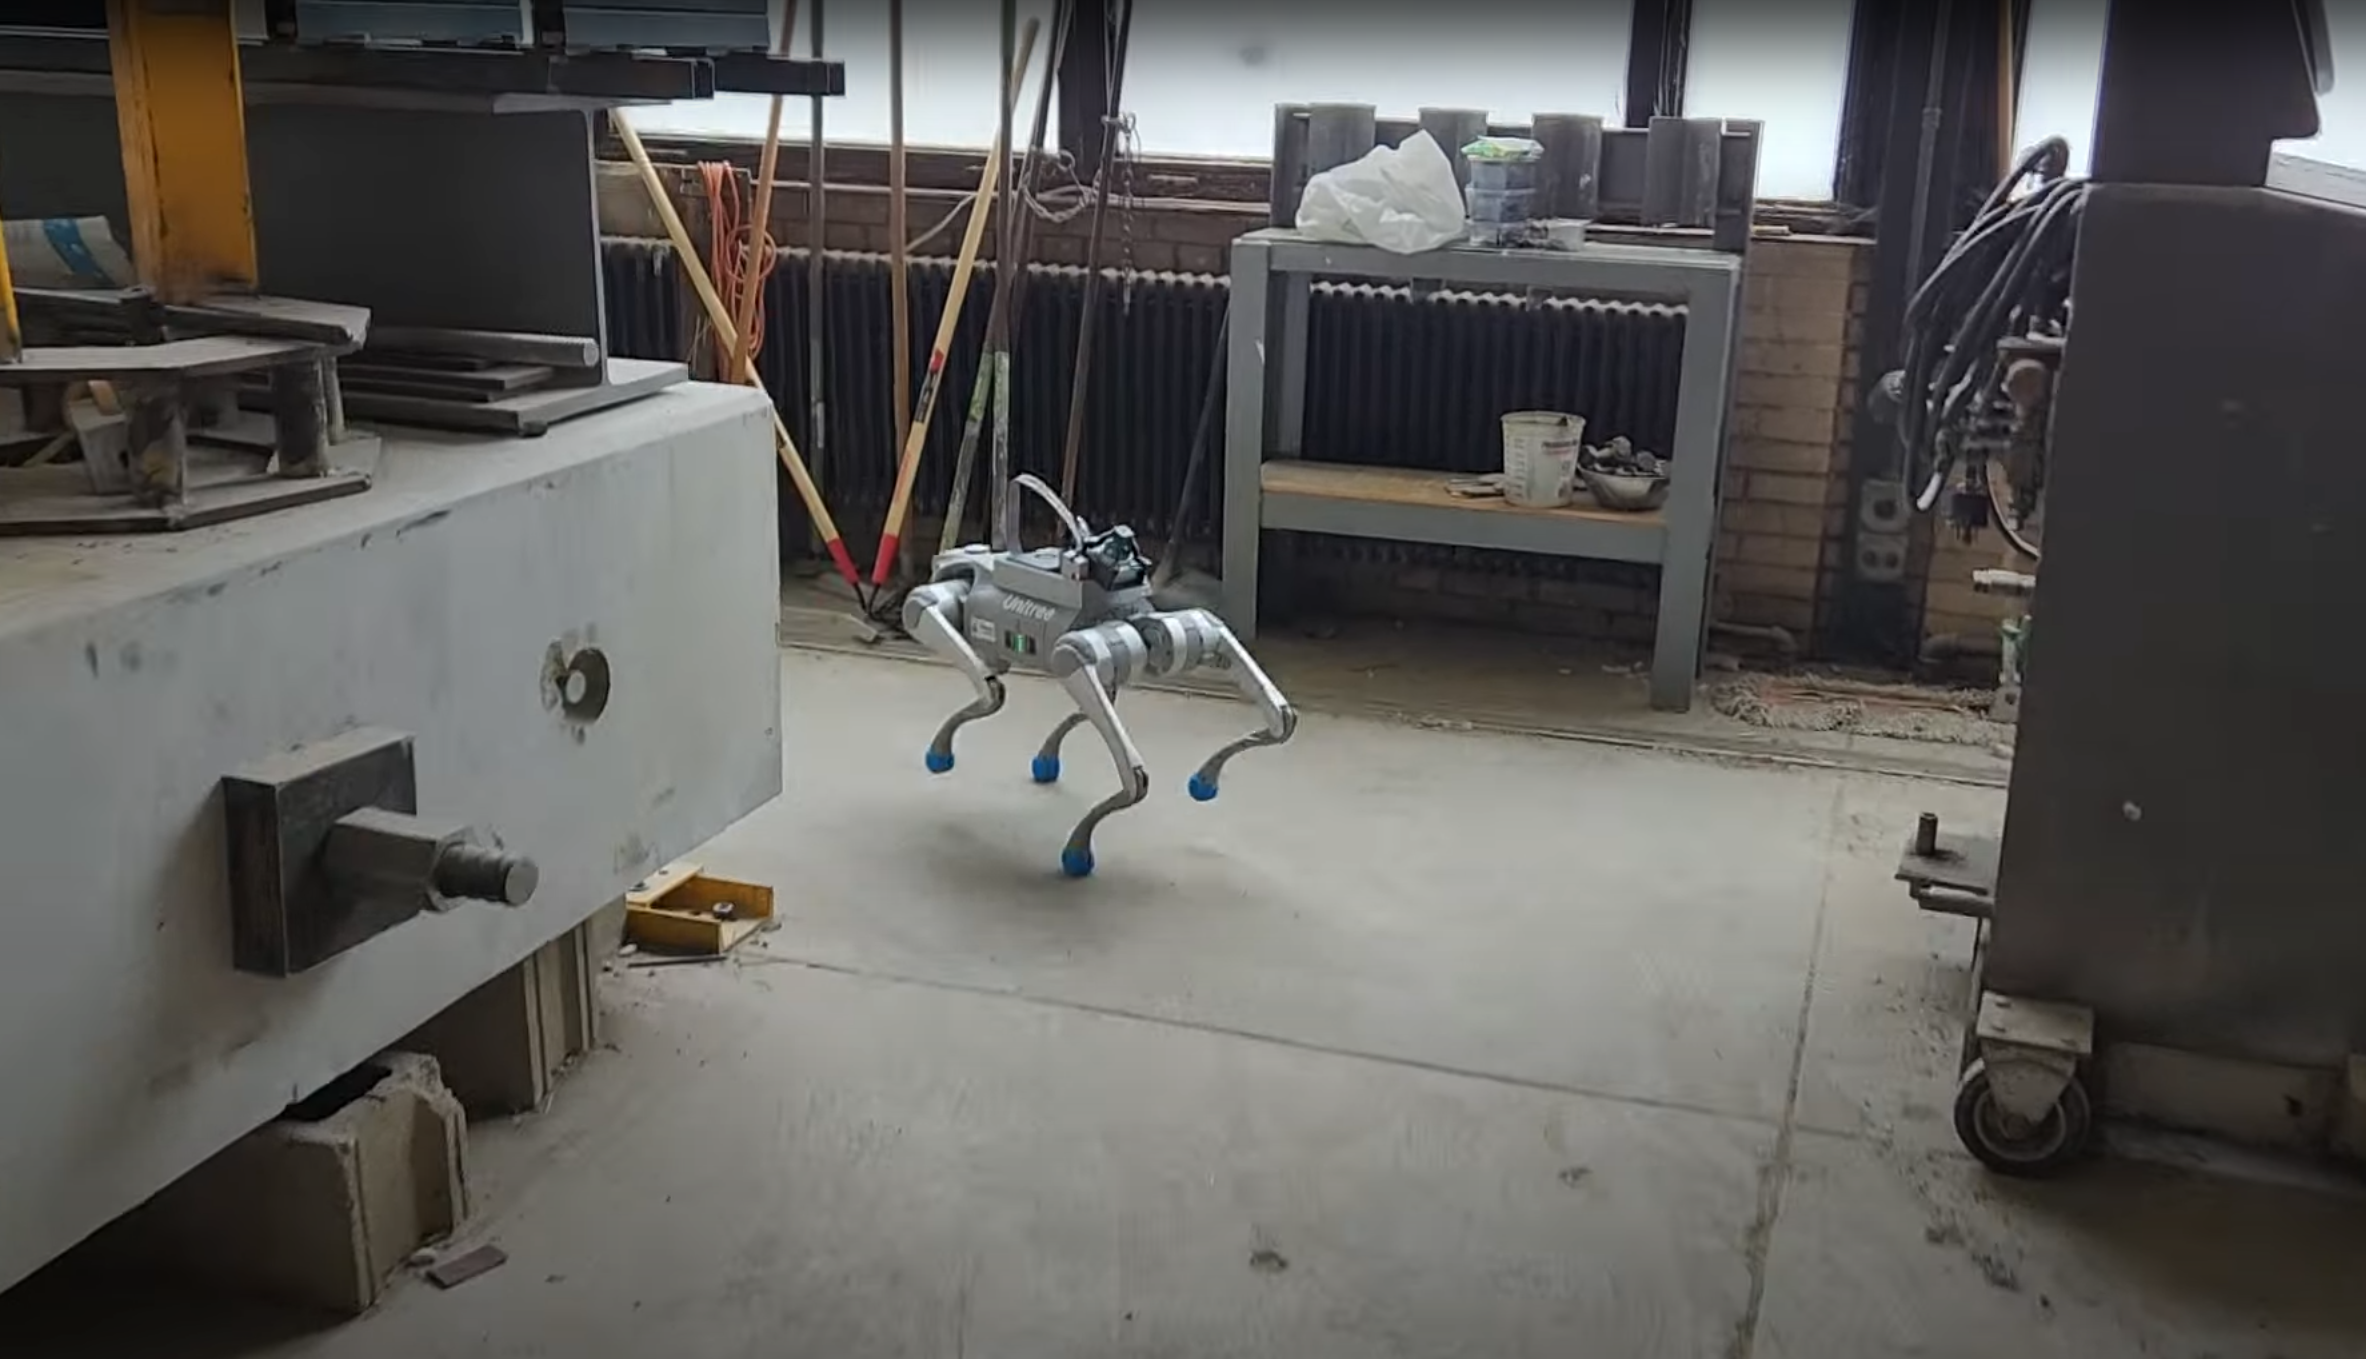
\includegraphics[width=0.7\textwidth]{Images/GO2_exploring_alumni.png}
            \caption{Unitree GO2 during a test exploration of the Alumni Hall at IIT}
            \label{fig:tare_iit_exploration}
        \end{figure}

        

        \begin{figure}[H]
            \centering
            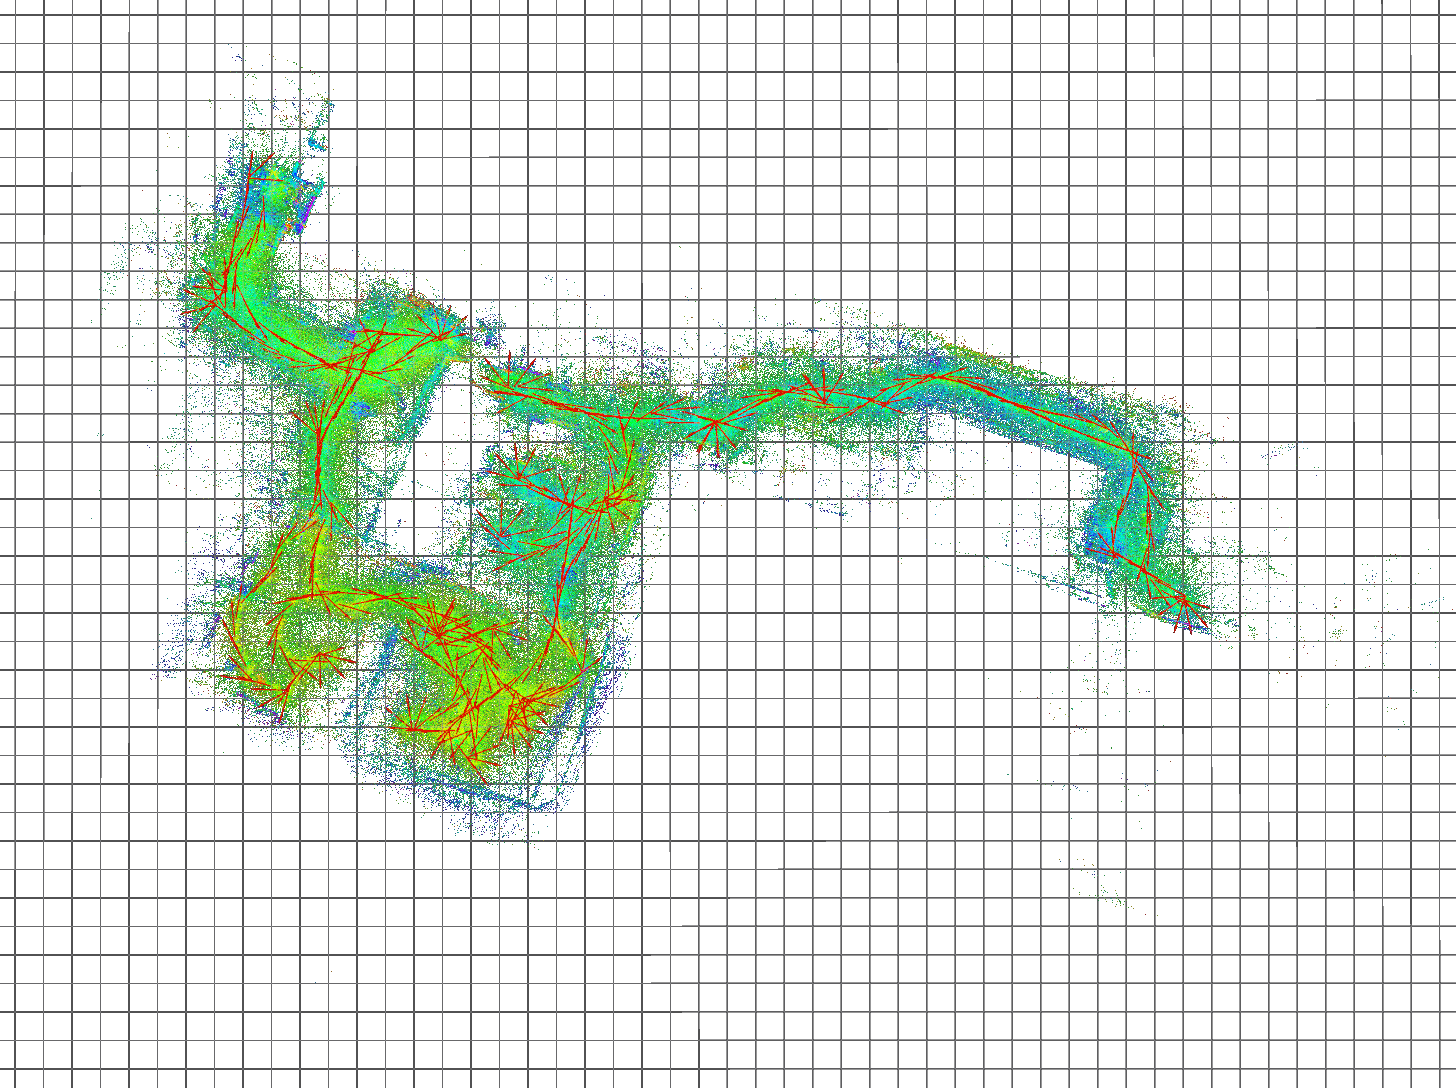
\includegraphics[width=0.95\textwidth]{Images/map_explore_alumni_no_bg.png}
            \caption{Top-down view of the point cloud captured by the GO2 during the exploration of the Alumni Hall at IIT, the grid has a cell size of 1m, the red arrows represent the odometry of the robot at various times}
            \label{fig:tare_iit_map}
        \end{figure}


        % TODO : explain the viewpoint selection with a figure 

        
        \subsubsection{MUI-TARE planner}
        % multi agent exploration

        The MUI-TARE planner \cite{yan2023mui} (Multi-agent TARE with Unknown Initial position) is an extended version of the previously described TARE planner that was used by the CMU team during the multi robot exploration stage of the DARPA SubT challenge. It uses AutoMerge \cite{yin2023automerge}, a framework meant for merging multiple large scale point clouds. MUI-TARE follows the hierarchical exploration strategy of TARE, where the entire exploration path is considered, maximizing the exploration rate.

        Until maps get initially merged, and their relative positions to one another is unknown, each agent plans its exploration independently. Once the maps are merged, the agents then cooperate in the exploration effort, by continuously sharing their maps. If communication is lost, the agents will resynchronize their maps by going back to a known meeting point. The meeting point is continuously updated while communications are active, but only after a certain amount of time has passed without communication will the agents go back to the last known meeting point. This ensures that the agents can continue to explore distant areas without having to go back to the meeting point too often. 


        As a simulation environment is provided, the MUI-TARE planner was first tested in simulation, allowing myself to understand the planner and to test the planner in a controlled environment. Such test can be seen in Figure \ref{fig:mui_tare_simulation}. The simulation environment is provided as a Docker image



        \begin{figure}
            \centering
            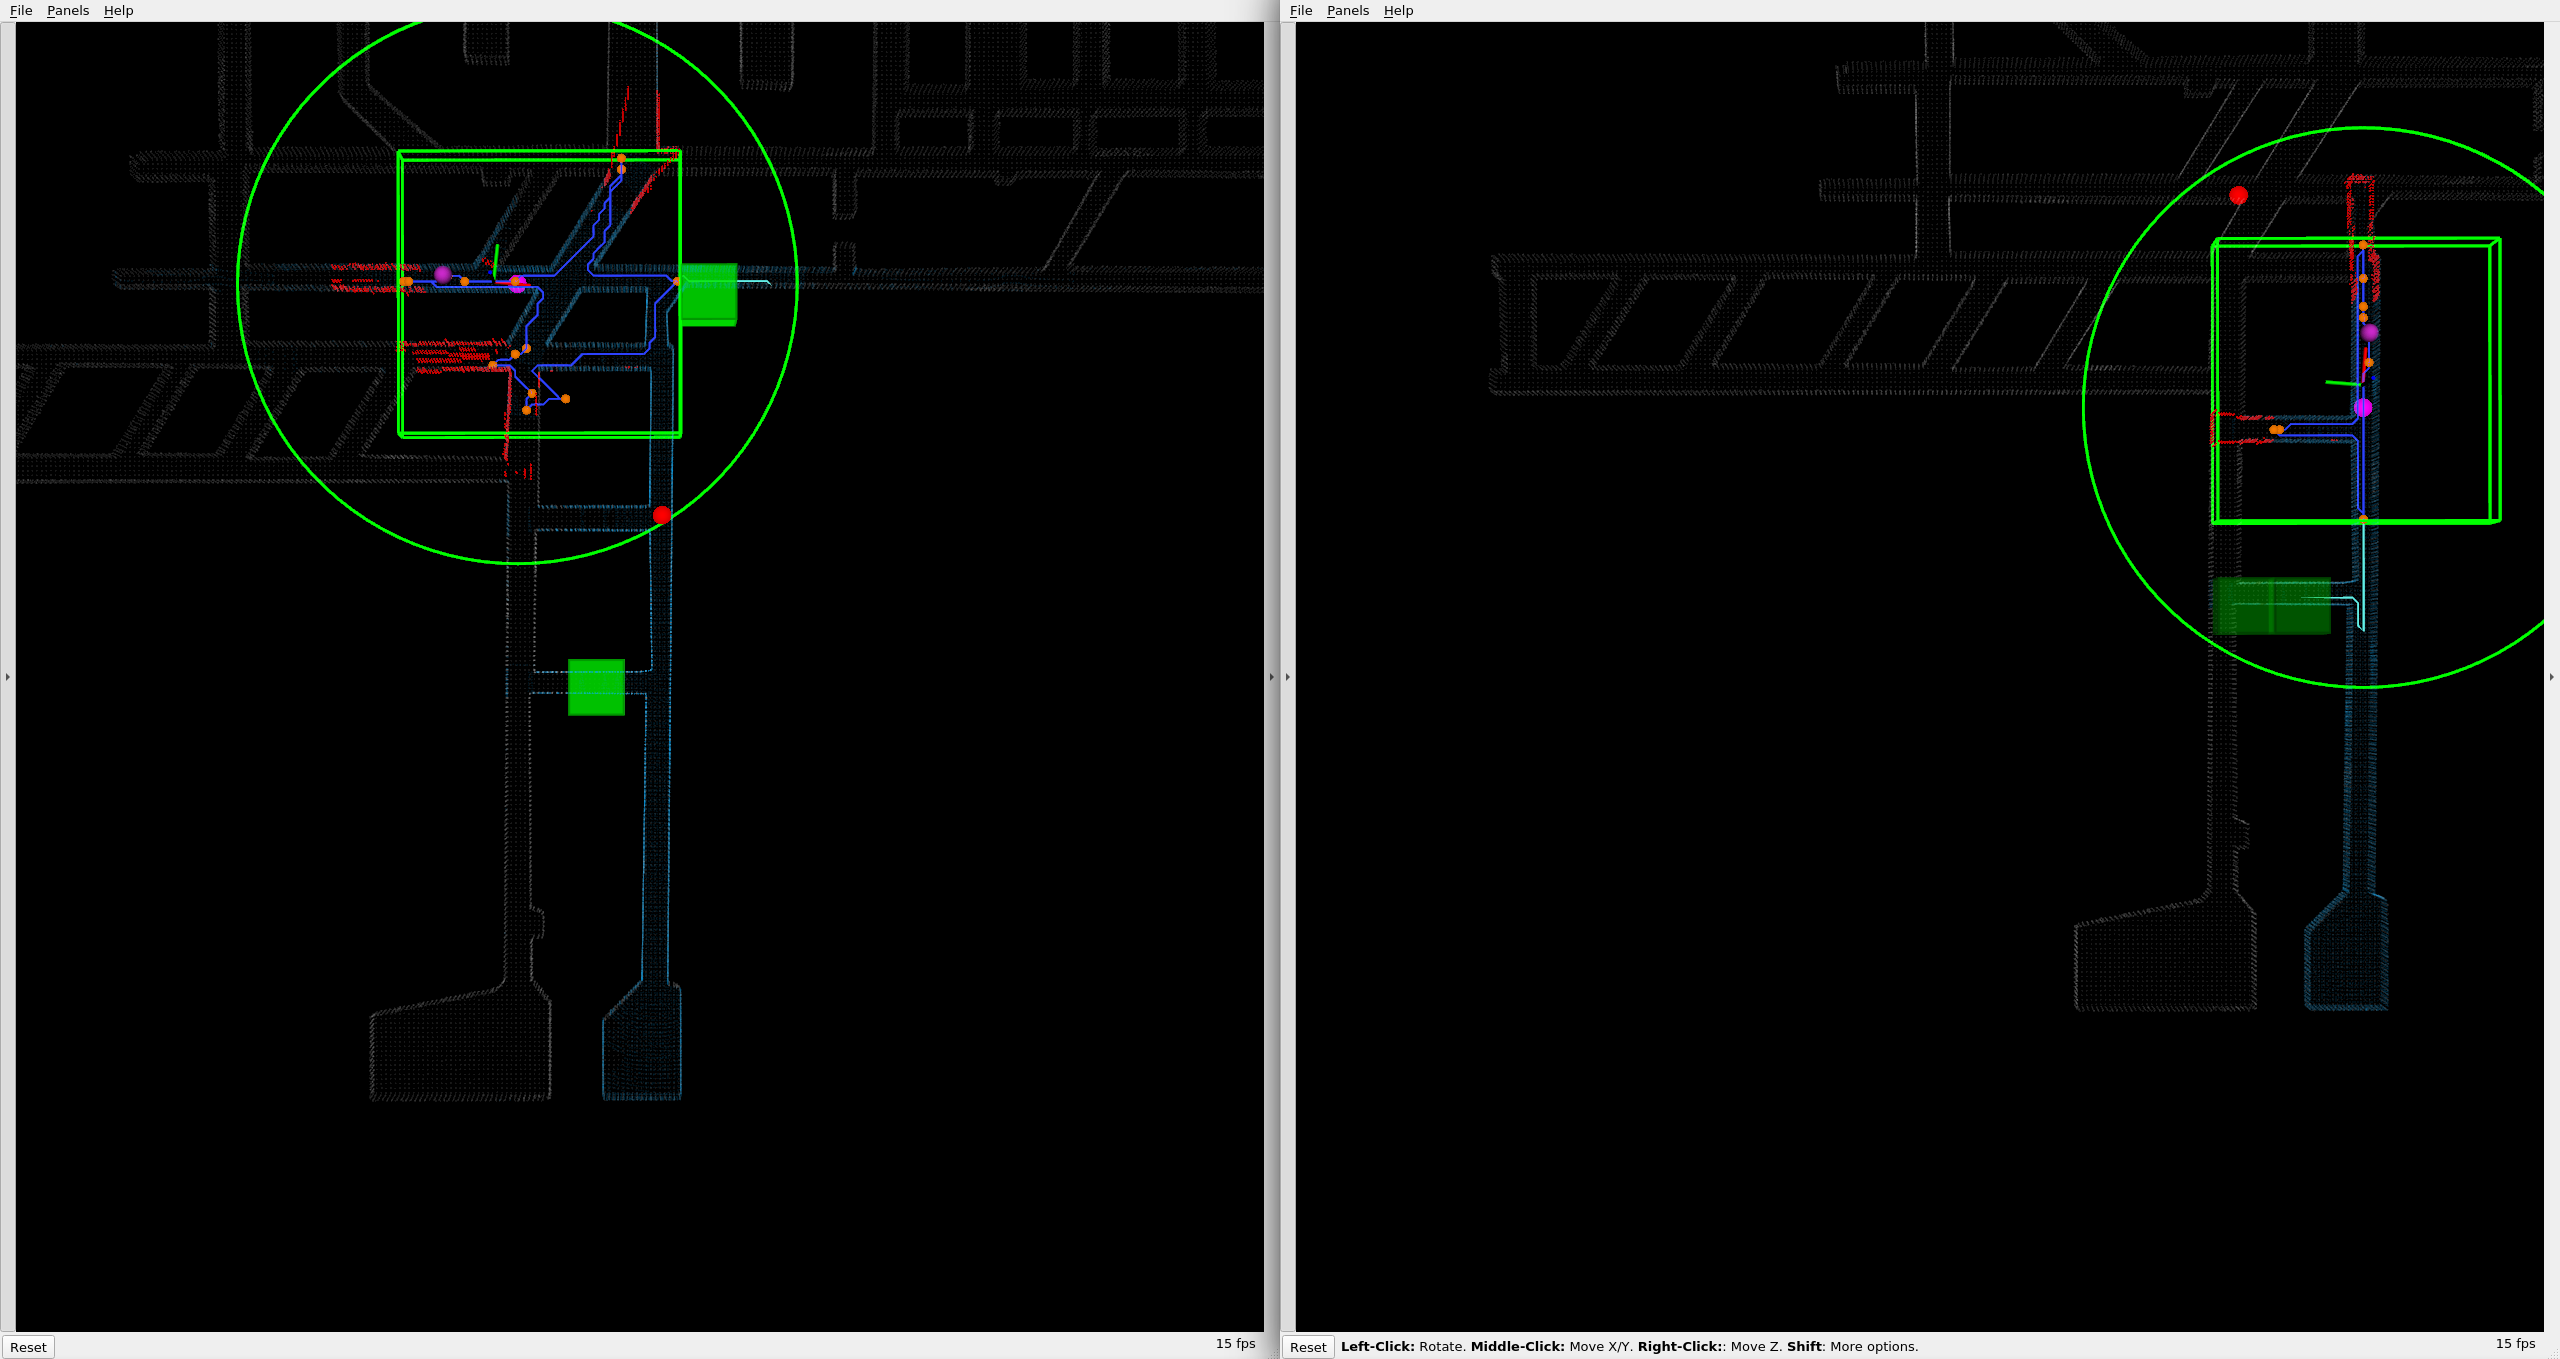
\includegraphics[width=0.95\textwidth]{Images/mtare_sim.png}
            \caption{Simulation of two agents exploring a tunnel environment, the agents' simulated communication ranges are represented by the green circles}
            \label{fig:mui_tare_simulation}
        \end{figure}

        While this algorithm was designed for the DARPA SubT challenge, it can be used in other exploration scenarios, such as the exploration of a large building in construction. That is why efforts were made to make the planner compatible with the quadruped and wheeled platforms. However, its high complexity and it's need to run a combination of ROS1 and ROS2 nodes made it difficult to integrate. Additionally, the communication method used during the DARPA SubT challenge was not disclosed, and time constraints made it impossible to implement a communication method that would work. We considered mesh networks, like the one used by the LoRaWAN \cite{rahman2020lorawan} protocol, but the high latency and low bandwidth made in unsuitable to send pint clouds. Some teams solutions were provided \cite{roucek2021system} but often rely on expensive and complicated hardware, often having multiple people per team dedicated to the communication aspect of the challenge.

        As such, the MUI-TARE planner was not integrated into the robots but remains a good candidate for the future. Additionally, the planner is proven to work in simulation, and has been tested during the DARPA SubT challenge, showcasing its robustness and efficiency. We believe this planner could thus be used in future exploration scenarios with the platforms already built, or with new platforms, by simply adding the necessary communication hardware and software. 

        %! This should be done but the work is too much for the time left
        %\subsubsection{Comparison of exploration algorithms}
        % metion the other exploration planners that are mentioned in the literature and how they compare to TARE and MTARE


    
\newpage
\section{Simulation}

    In robotics, simulation is a key part of the development process. Unlike traditional software development, the testing of algorithms needs to be done on the physical platform, which can be time consuming and costly. Simulation allows for the testing of algorithms in a controlled environment, where the behavior of the robot can be closely mimicked. It also removes any risks associated with testing on the physical platform, such as damaging the robot or causing injury. 

    \subsection{Choosing a simulation environment}

        To test the algorithms and the coordination of the different platforms, a simulation environment was needed. The choice of the simulation environment was based on the following criteria : being able to simulate multiple platforms, being able to simulate the sensors we had on the physical platforms, and the portability of the simulation environment.


        \subsubsection{Gazebo}
            Gazebo is a well known simulation environment in the robotics community. It is widely used and has a large community. It is open source and has a lot of plugins available, for simulation sensors, motion platforms and more. As I was already familiar with it, I first looked at it to build a crude simulation of the 6 wheeled platform. Thanks to the use of ROS2 and ROS2-control for the drive train, I was able to quickly build a simulation of the platform. 

            I was also able to find a working simulation of the Livox Mid-360 LIDAR sensor we chose for every platform. The package \cite{livox_lidar_simulation_fork} was a fork of the original simulation package from Livox \cite{livox_laser_simulation} and was modified to work with the specific LIDAR we are using.
            
            \begin{figure}[H]
                \centering
                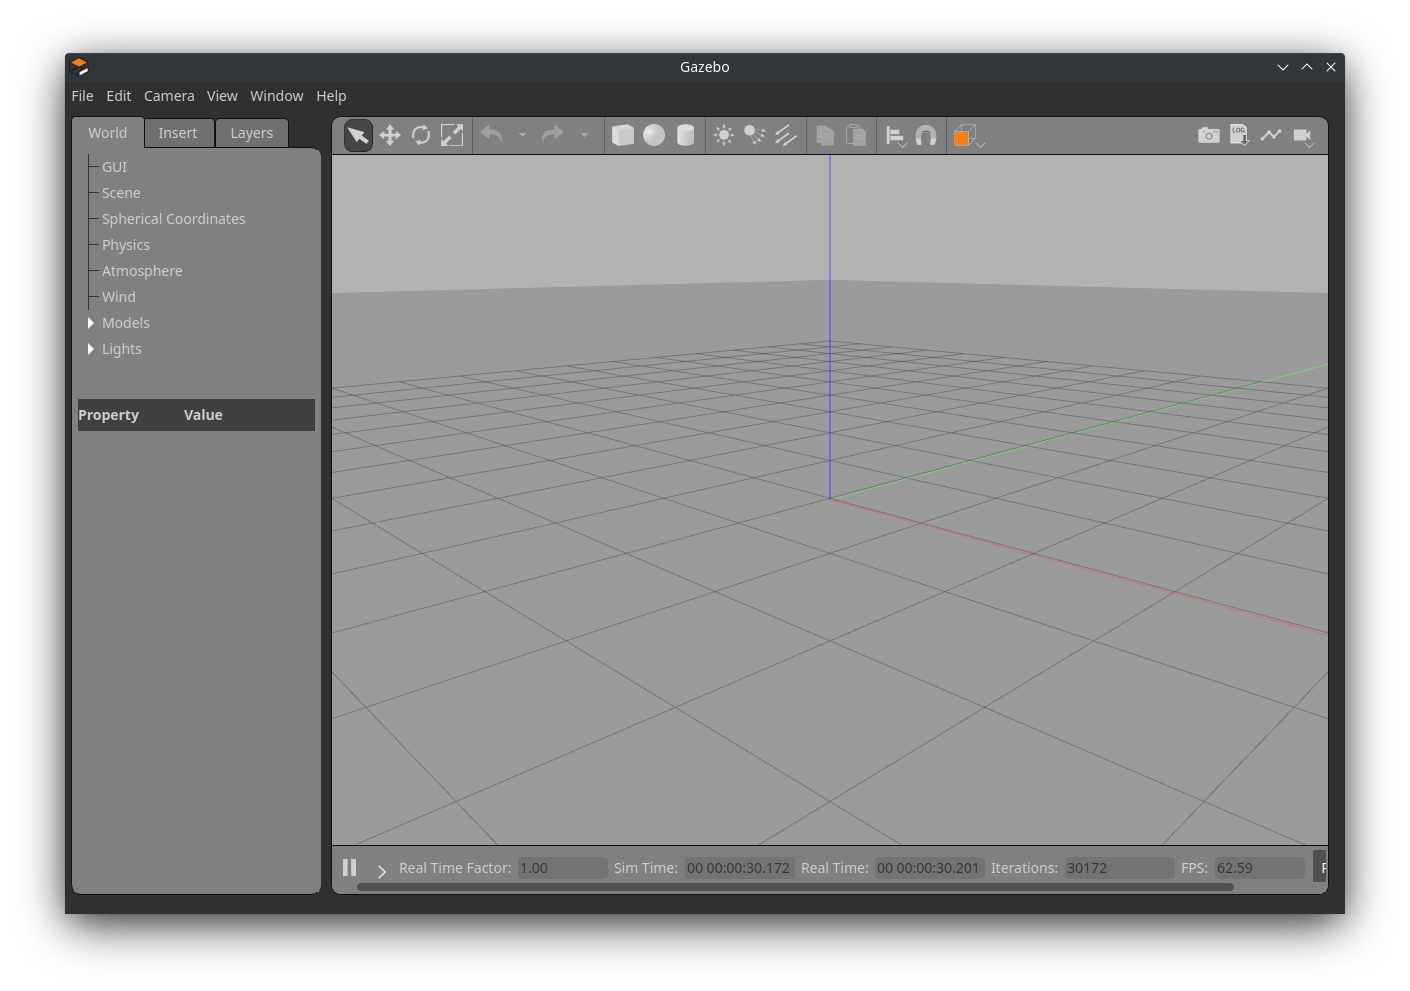
\includegraphics[width=0.7\textwidth]{Images/gazebo_interface.png}
                \caption{Gazebo classic interface, simulation environment in the center, toolbar on top, and the world tree on the left}
                \label{fig:gazebo_simulation}
            \end{figure}


        \subsubsection{Nvidia Isaac Sim}

            Isaac sim is a high fidelity simulation environment developed by Nvidia. This simulation environment uses a PhysX based physics engine and is able to simulate multiple platforms at once. It is also able to simulate sensors like cameras, LIDARs and IMUs. The main advantage of Isaac sim is its high fidelity and parallelization. However, this also brings a lot of complexity and the need for an RTX GPU to run it.
            
            \begin{figure}[H]
                \centering
                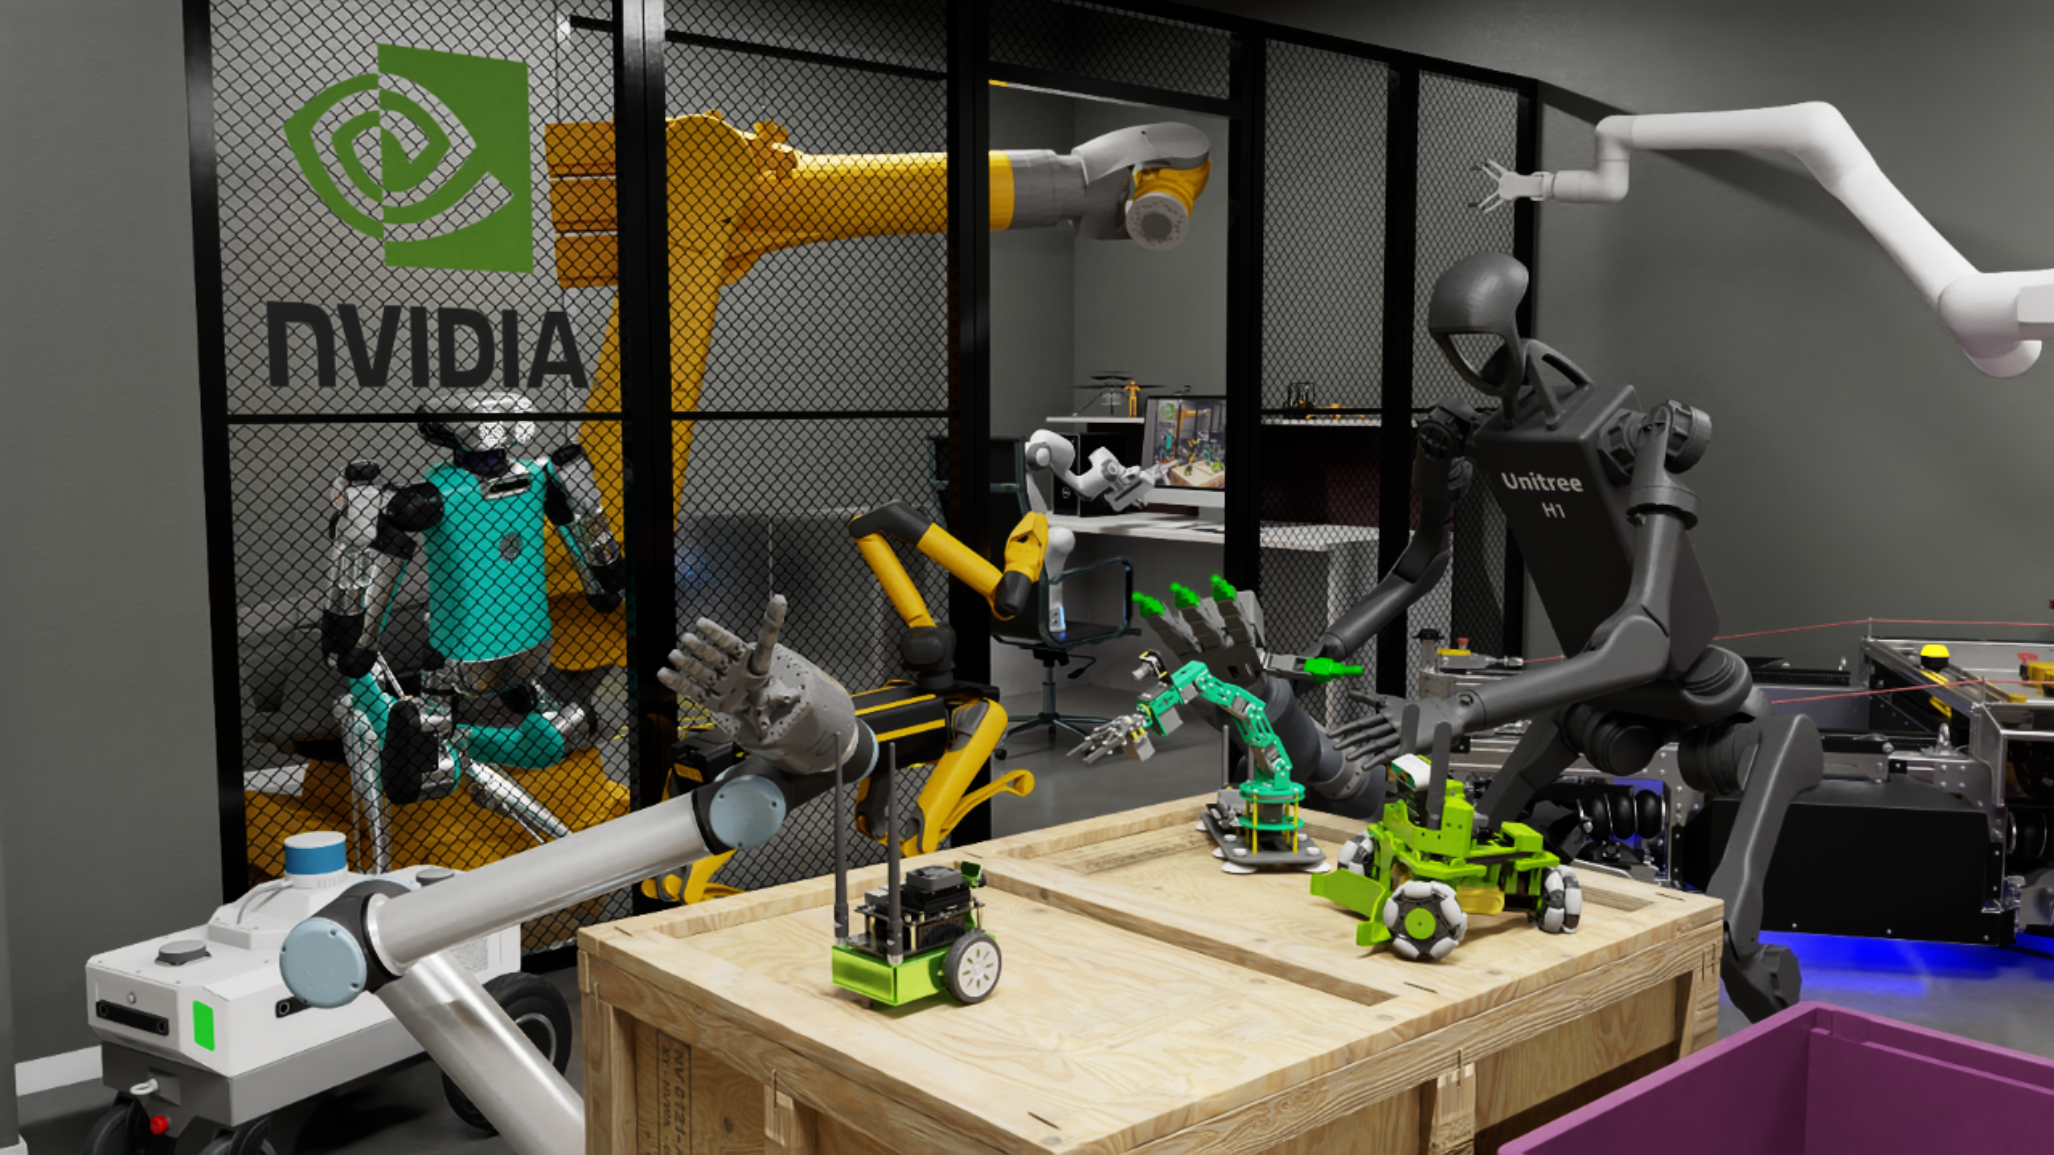
\includegraphics[width=0.69\textwidth]{Images/isaac_sim.png}
                \caption{View of some built-in robots in Isaac Sim}
                \label{fig:isaac_sim_robots}
            \end{figure}
            
            The high overhead, complexity, low portability and the fact that it was not open source made me choose Gazebo over Isaac sim for the simulation of the platforms.

            In addition, the LIDAR we are using has a non-repetitive pattern, which is not currently supported by Isaac sim and would have required a lot of work to simulate.

            I did experiment with Isaac sim to simulate the quadruped platform, as it was the most complex platform to simulate and there existed a simulation of the robot in Isaac sim.

            Some built-in robots in Isaac sim are shown in Figure \ref{fig:isaac_sim_robots}. We can also observe the high fidelity of the simulation environment and the lighting effects that Isaac Sim is capable of.

            I did end up experimenting with Isaac Sim for simulating the quadruped platform, as examples are available for reinforcement learning of locomotion for quadrupeds. The simulation of the quadruped platform in Isaac Sim can be seen in Figure \ref{fig:isaac_sim_quadruped}.



            \begin{figure}[H]
                \centering
                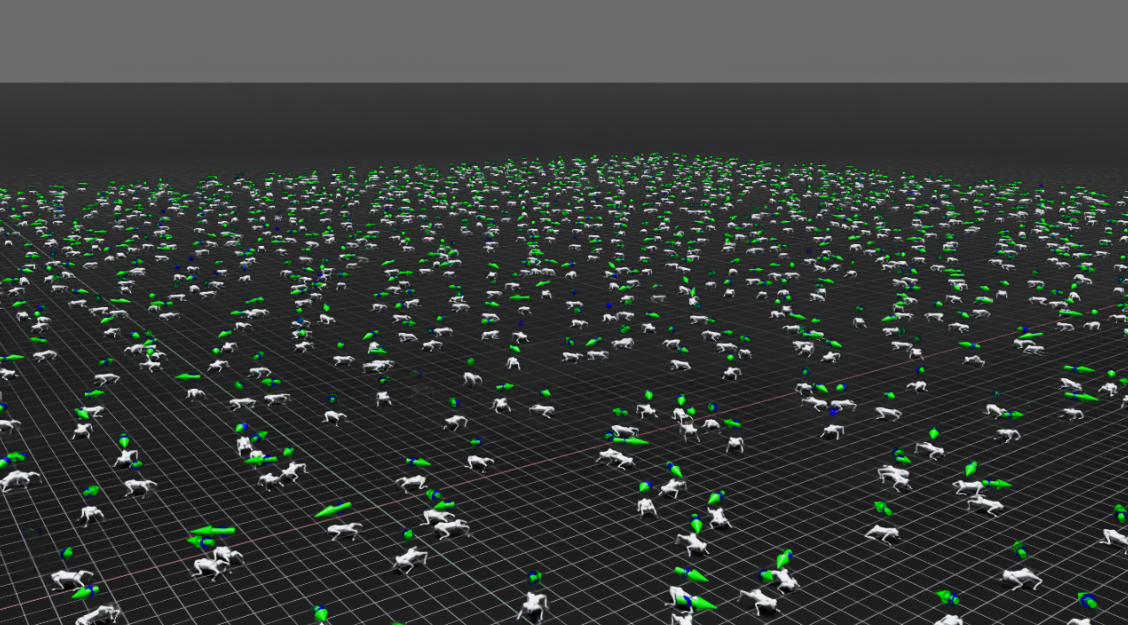
\includegraphics[width=0.5\textwidth]{Images/go2_rl_training.png}
                \caption{Quadruped platform reinforcement learning training in Isaac Sim}
                \label{fig:isaac_sim_quadruped}
            \end{figure}

        \subsubsection{Simulation using game engines}

            Other researchers have used game engines like Unity or Unreal Engine for simulation. These engines offer high graphical fidelity while maintaining a high level of performance. One example is the GO2 and Diablo simulations that researchers at Carnegie Mellon University have done in Unity as can be seen in Figure \ref{fig:unity_simulation}. This simulation uses \texttt{ros\_tcp\_endpoint}, a ROS package that allows for communication between ROS and Unity. The Unity simulation requires the \texttt{ros\_tcp\_connector} unity package, this establishes a connection between the ROS2 node and the Unity simulation.
            \begin{figure}[h]
                \centering
                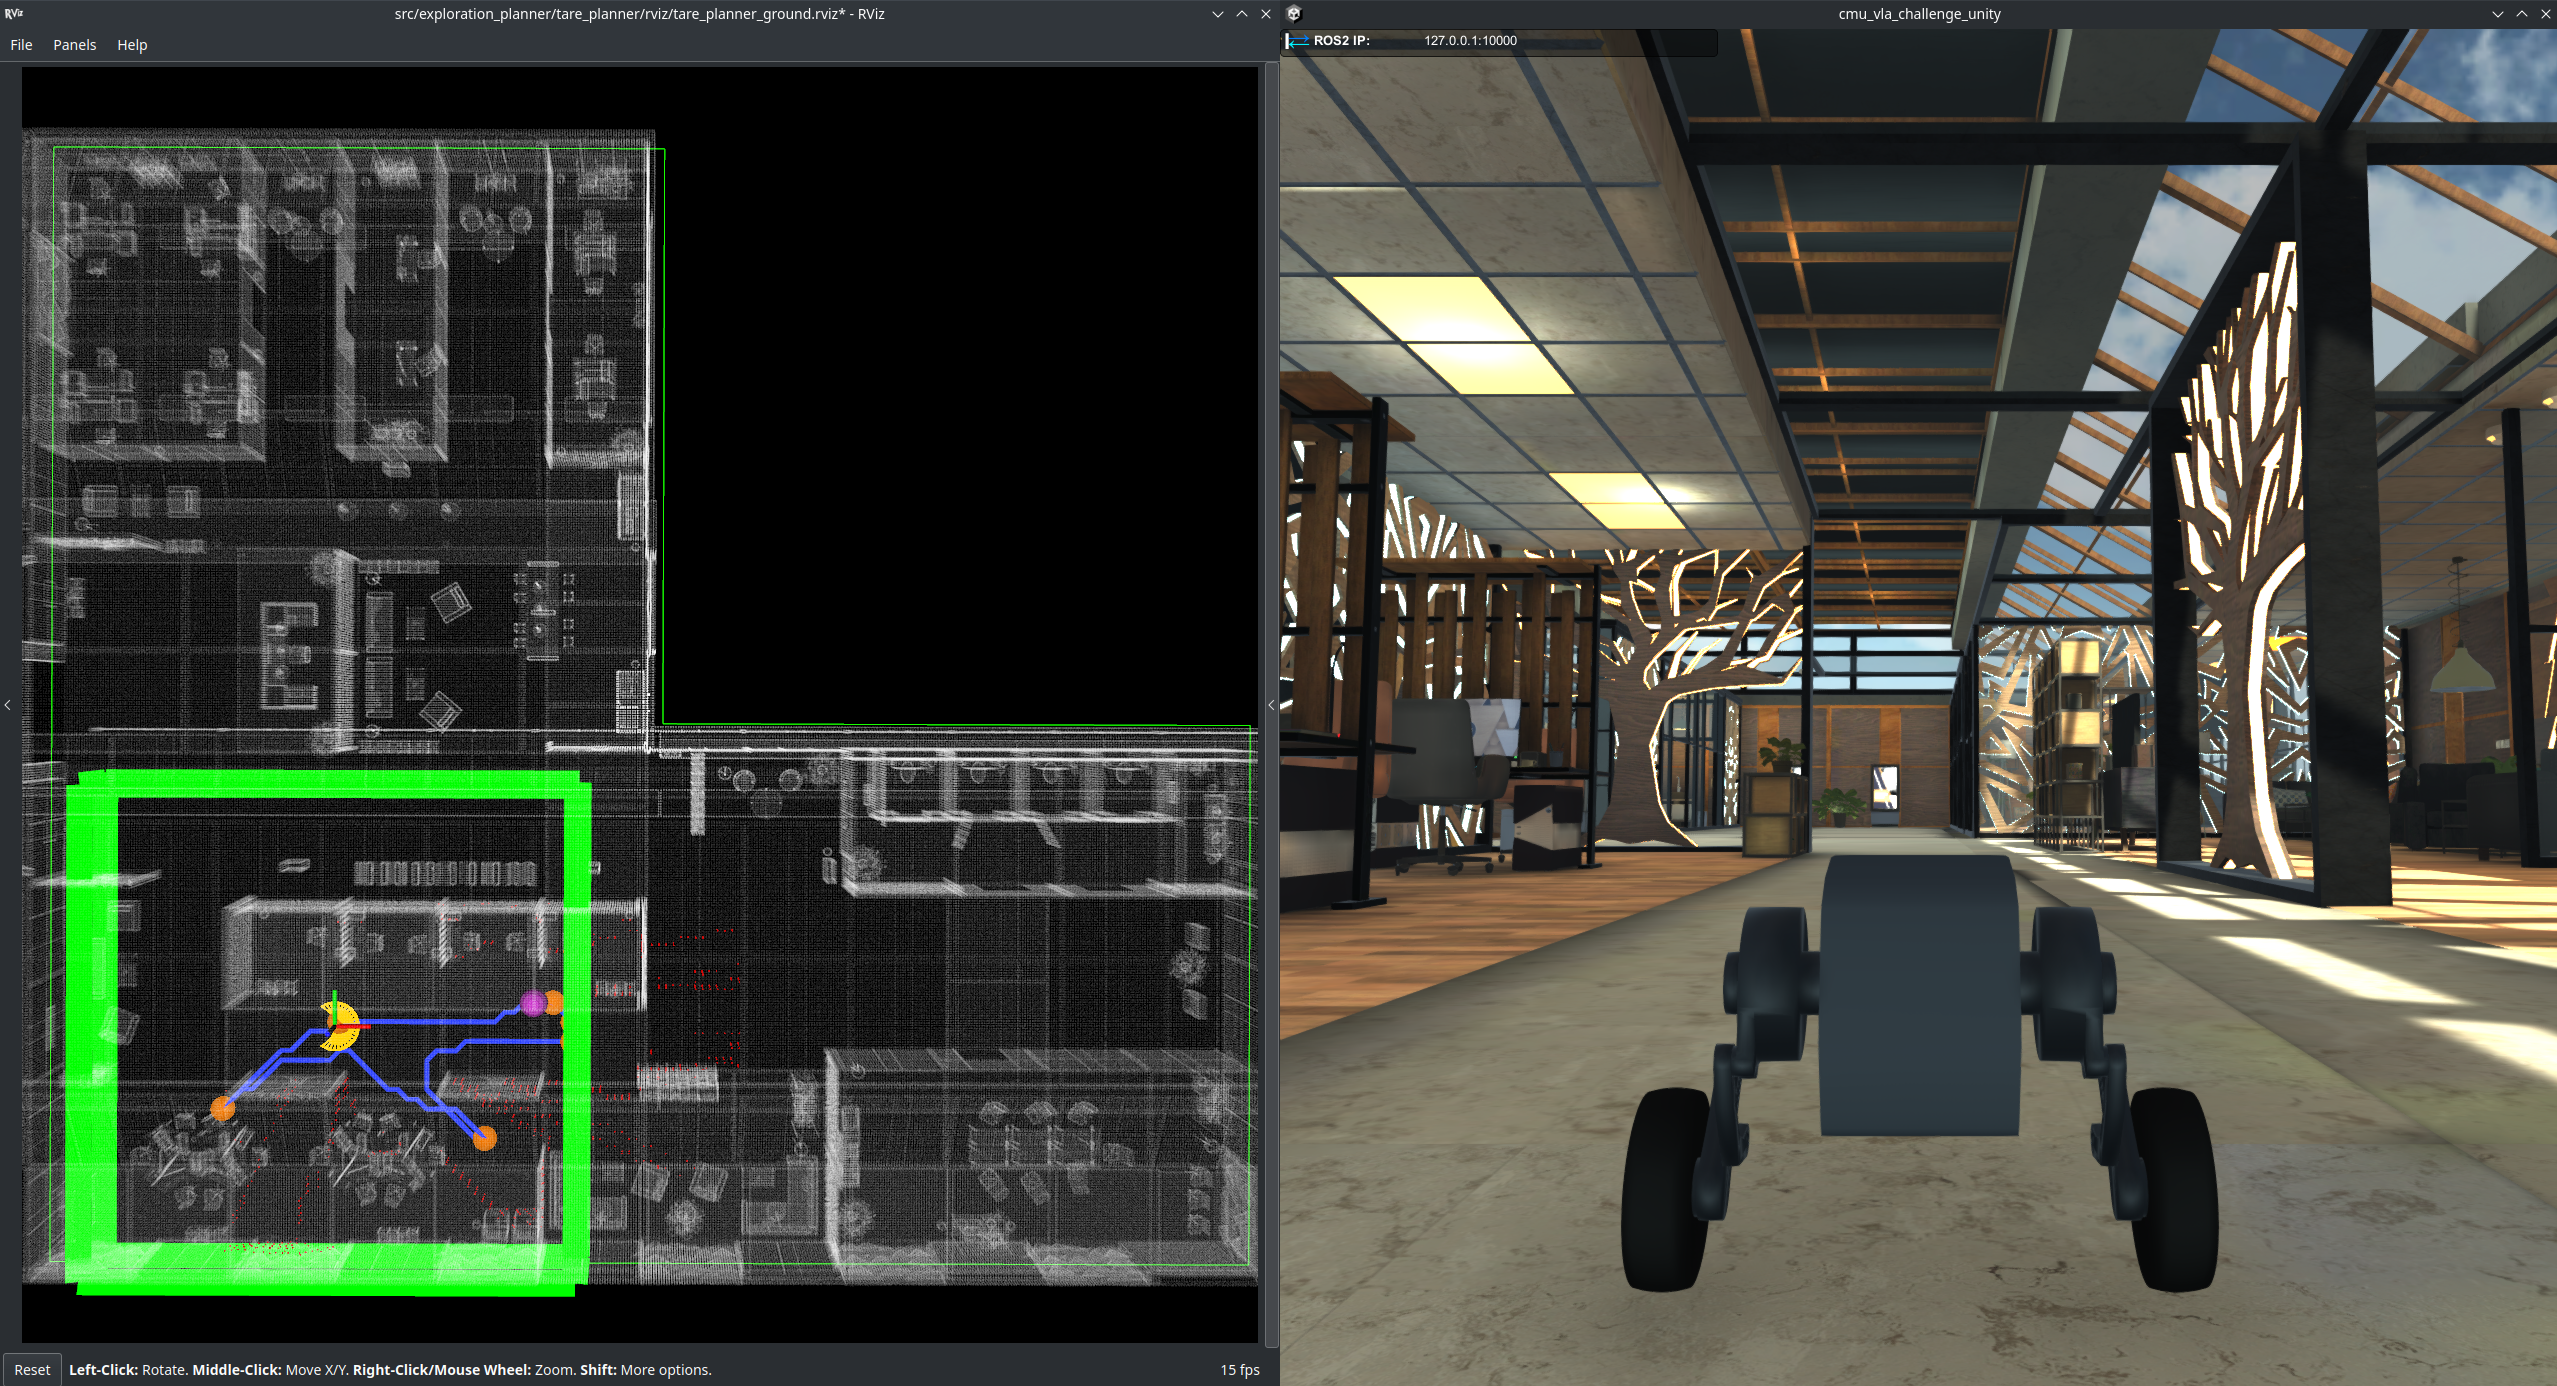
\includegraphics[width=0.75\textwidth]{Images/Unity_simulation.png}
                \caption{Simulations of the GO2 and Diablo platforms in Unity on the right, with the data generated and tare planner running visualized in RVIZ2 on the left}
                \label{fig:unity_simulation}
            \end{figure}

            The main advantage of using a game engine for such simulation is the high fidelity that can be achieved, which is sometimes necessary for tasks such as machine vision or reinforcement learning. However, the complexity of the setup and the need to implement every sensor and actuator can be a drawback. Additionally, the physics engines used in game engines are optimized for games and not for accuracy, which can be a problem for some applications.

            The long and complex setup of the Unity simulation is the reason why I did not choose this method for the simulation of the platforms.

    \subsection{Simulating sensors}

        To have an accurate simulation that closely mimics the physical platform, the sensors on the physical platform need to be simulated. The sensors that were simulated were the LIDAR and the IMU. Even though not necessary, the camera and depth camera were also simulated to have a complete simulation of the platform.

        \subsubsection{LIDAR}

        Gazebo comes with a way of simulating 2D LIDARs, but no built-in way of simulating 3D LIDARs. This functionality was introduced in a recent version of Gazebo, but it's incompatibility with older Gazebo worlds and robot model made it difficult to justify changing version when a lot of work was already invested in the simulation. Moreover, the LIDAR we are using has a non-repetitive pattern, which is not currently supported by Gazebo build in GPU LIDAR that is present in the newer version. 
        
                \begin{figure}[H]
                    \centering
                    \subfigure[Gazebo simulation environment]{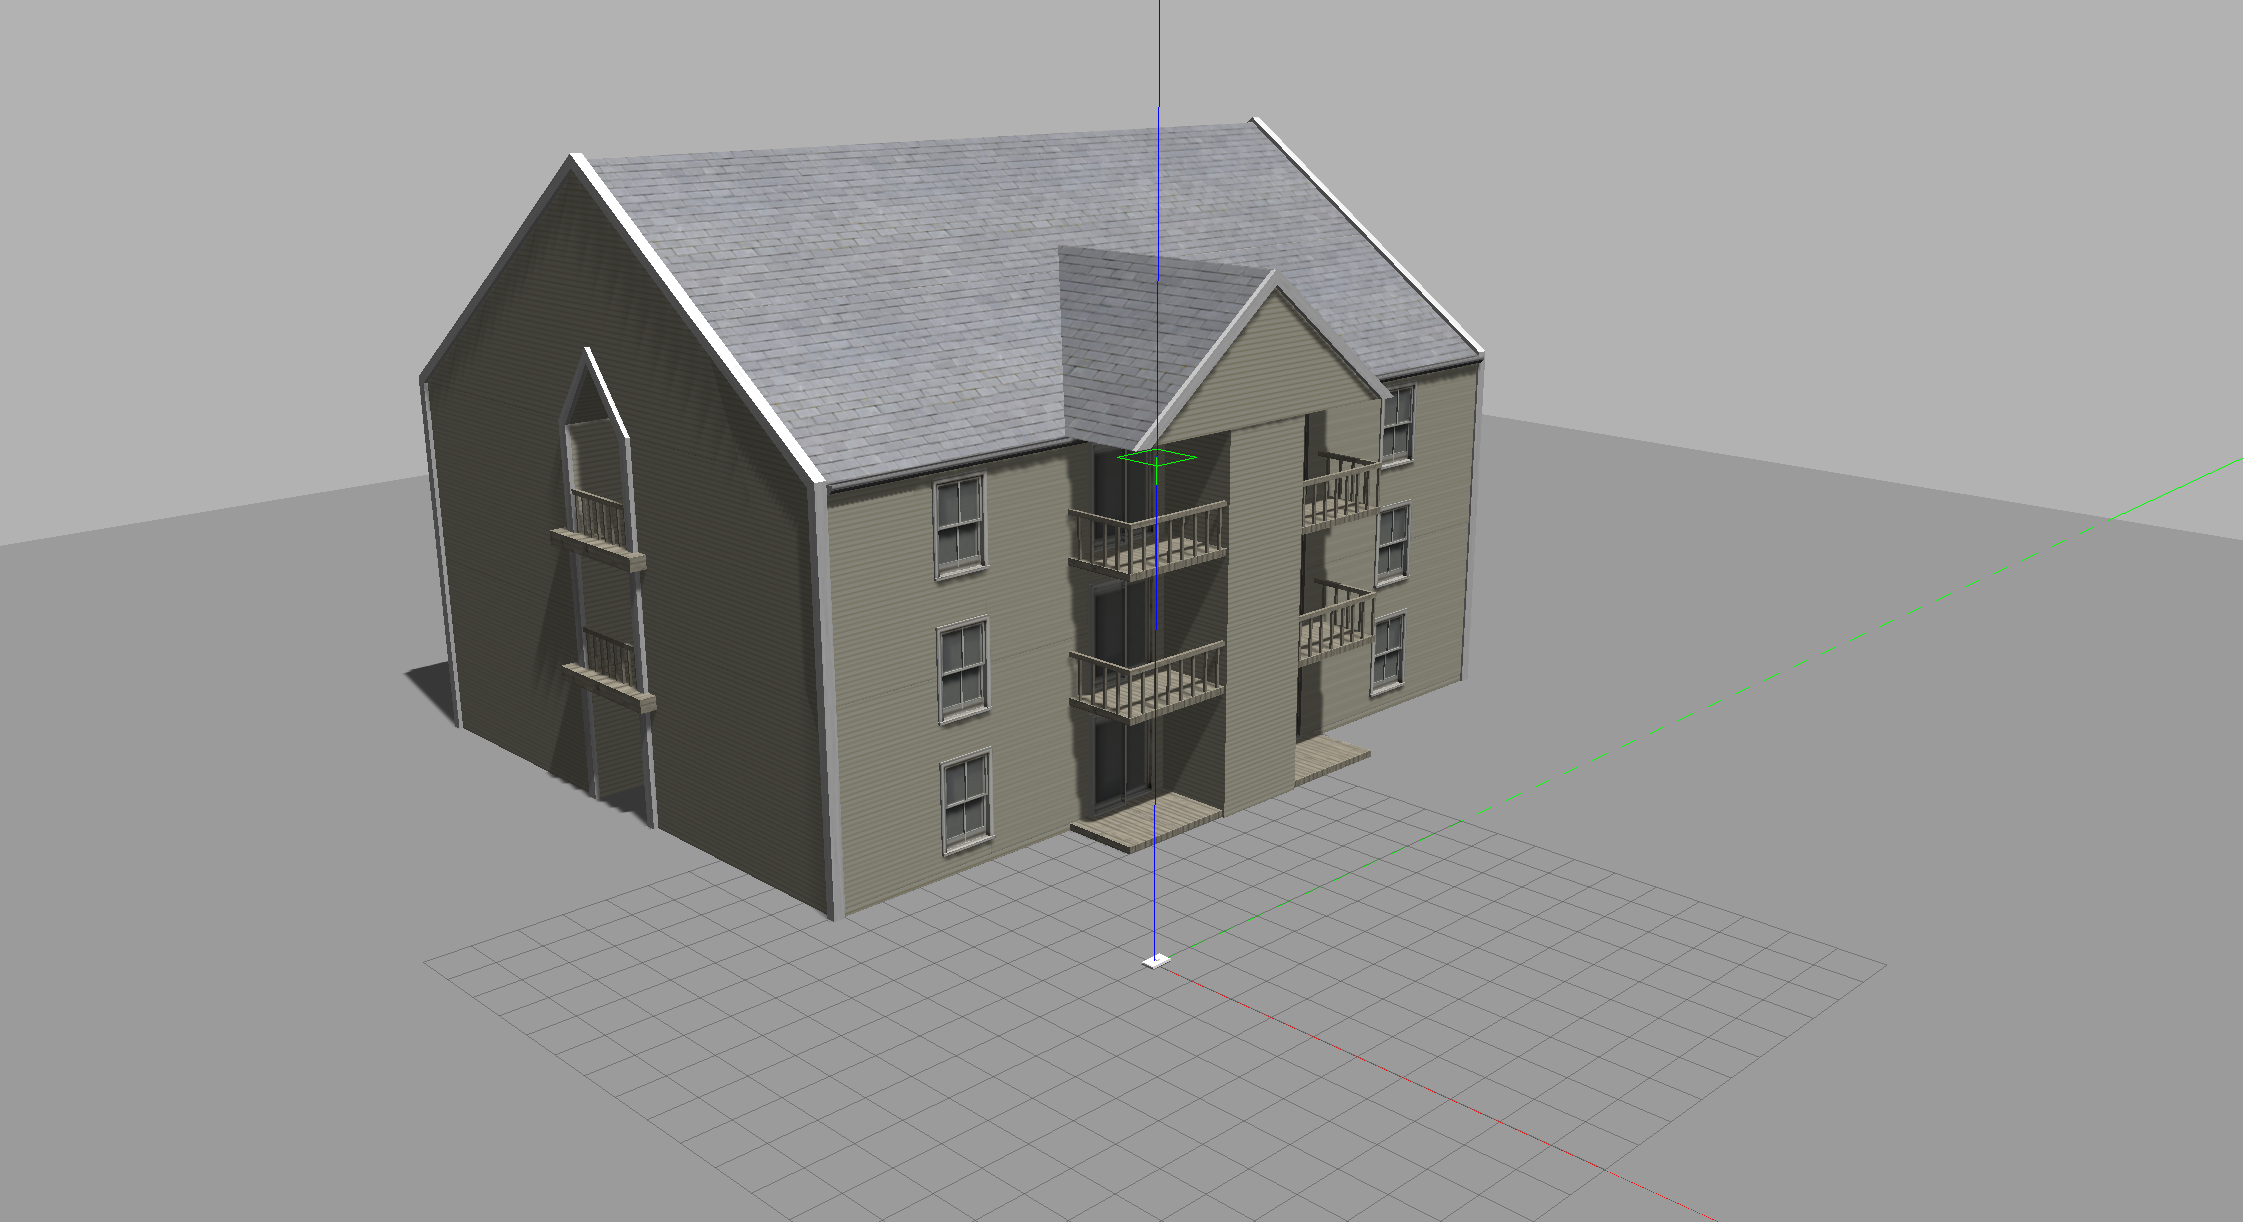
\includegraphics[height=0.25\textwidth]{Images/croped lidar simulation gazebo.png}}
                    \subfigure[Point cloud from simulated LIDAR]{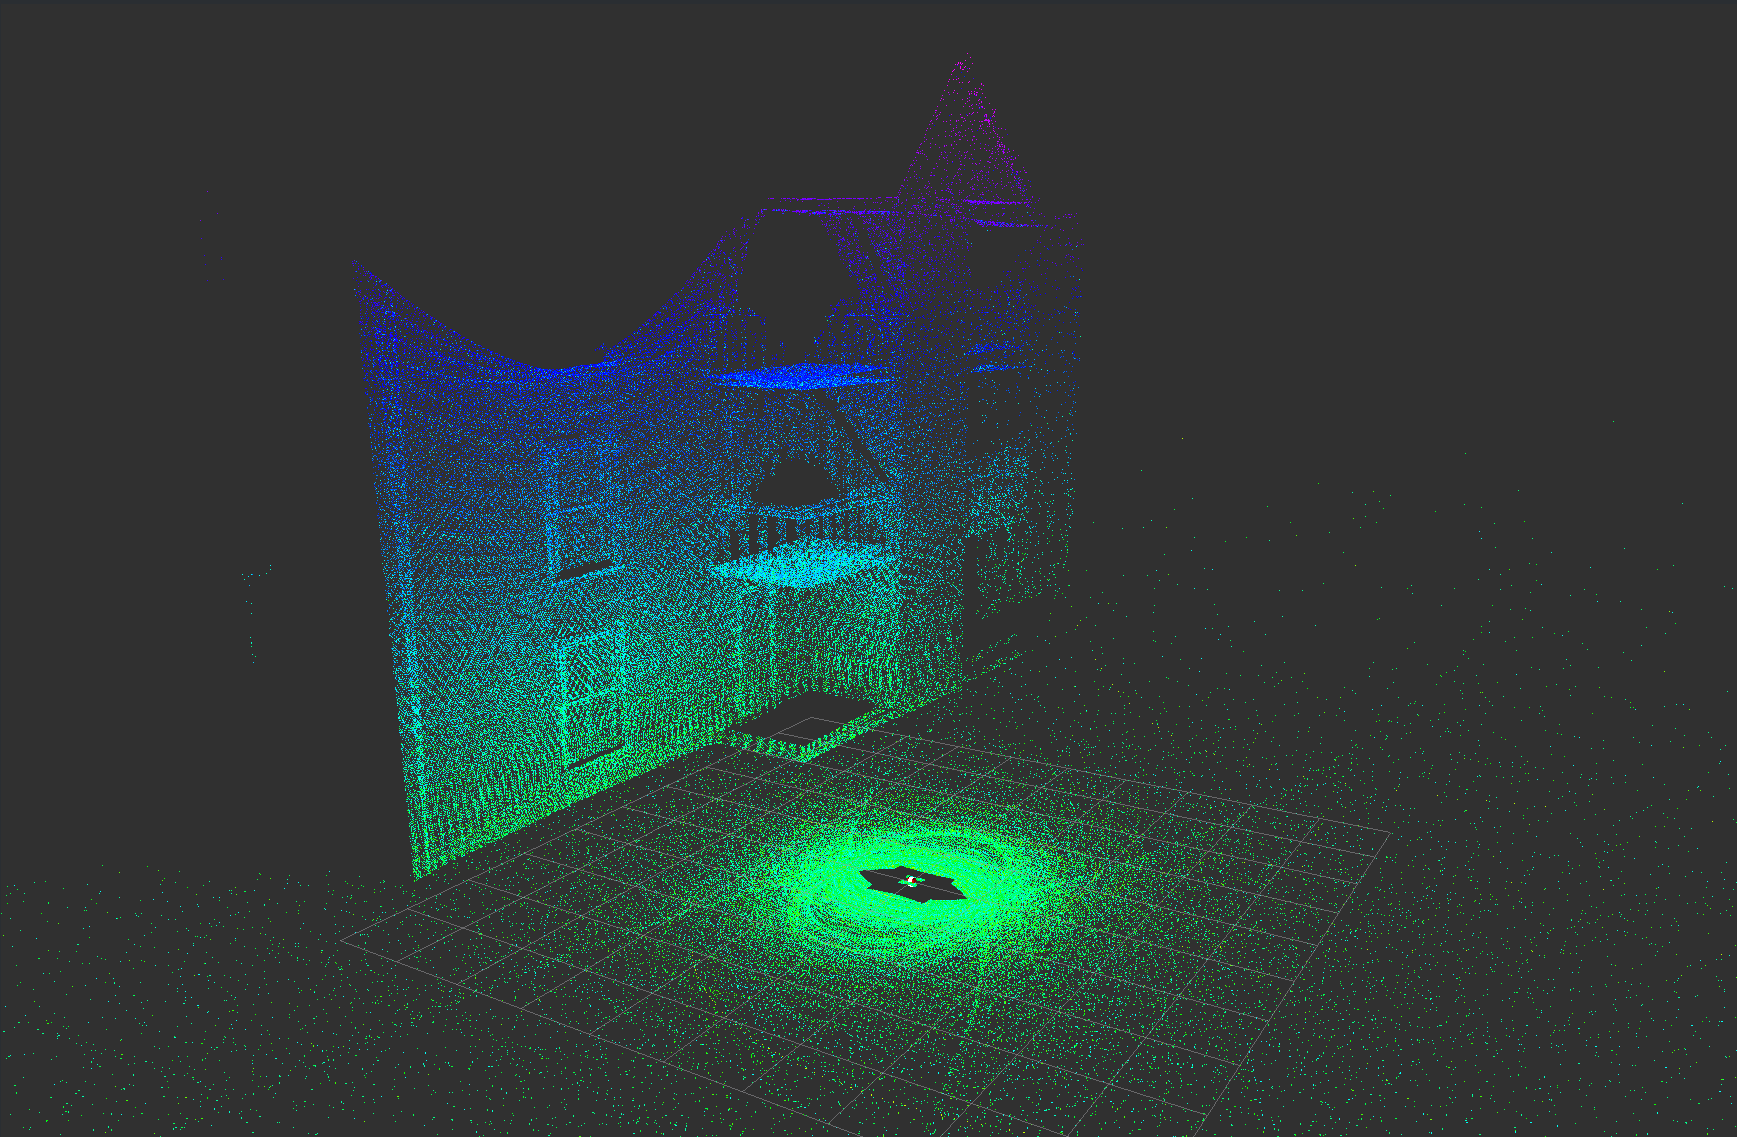
\includegraphics[height=0.25\textwidth]{Images/croped lidar simulation rviz2.png}}
                    \caption{Simulated LIDAR in Gazebo and point cloud in RVIZ2}
                    \label{fig:lidar_simulation}
                \end{figure}
        
        That is why I relied on a fork \cite{livox_laser_simulation_RO2} of Livox original simulation plugin was used. This plugin offers a simulation of the Mid-360 LIDAR that we are using, and offers a way to simulate the exact messages that the LIDAR driver would send. Additionally, the package offers a close simulation of the non repeating pattern of the LIDAR by using recorded laser angle measured from the real LIDAR and using this data to simulate the LIDAR in Gazebo. As we can see in Figure \ref{fig:lidar_simulation}, the LIDAR simulation is close to the real LIDAR point cloud, and does not feature repeating line of traditional multi-line 3D LIDARs. No effort were made to make this simulation of the LIDAR more accurate, however, we can note that in Figure \ref{fig:lidar_simulation}, the point cloud does not feature the same blind spots as the real LIDAR as can be seen in Figure \ref{fig:real_lidar_scan}. This is a point that could be improved in the future.


        \begin{figure}[H]
            \centering
            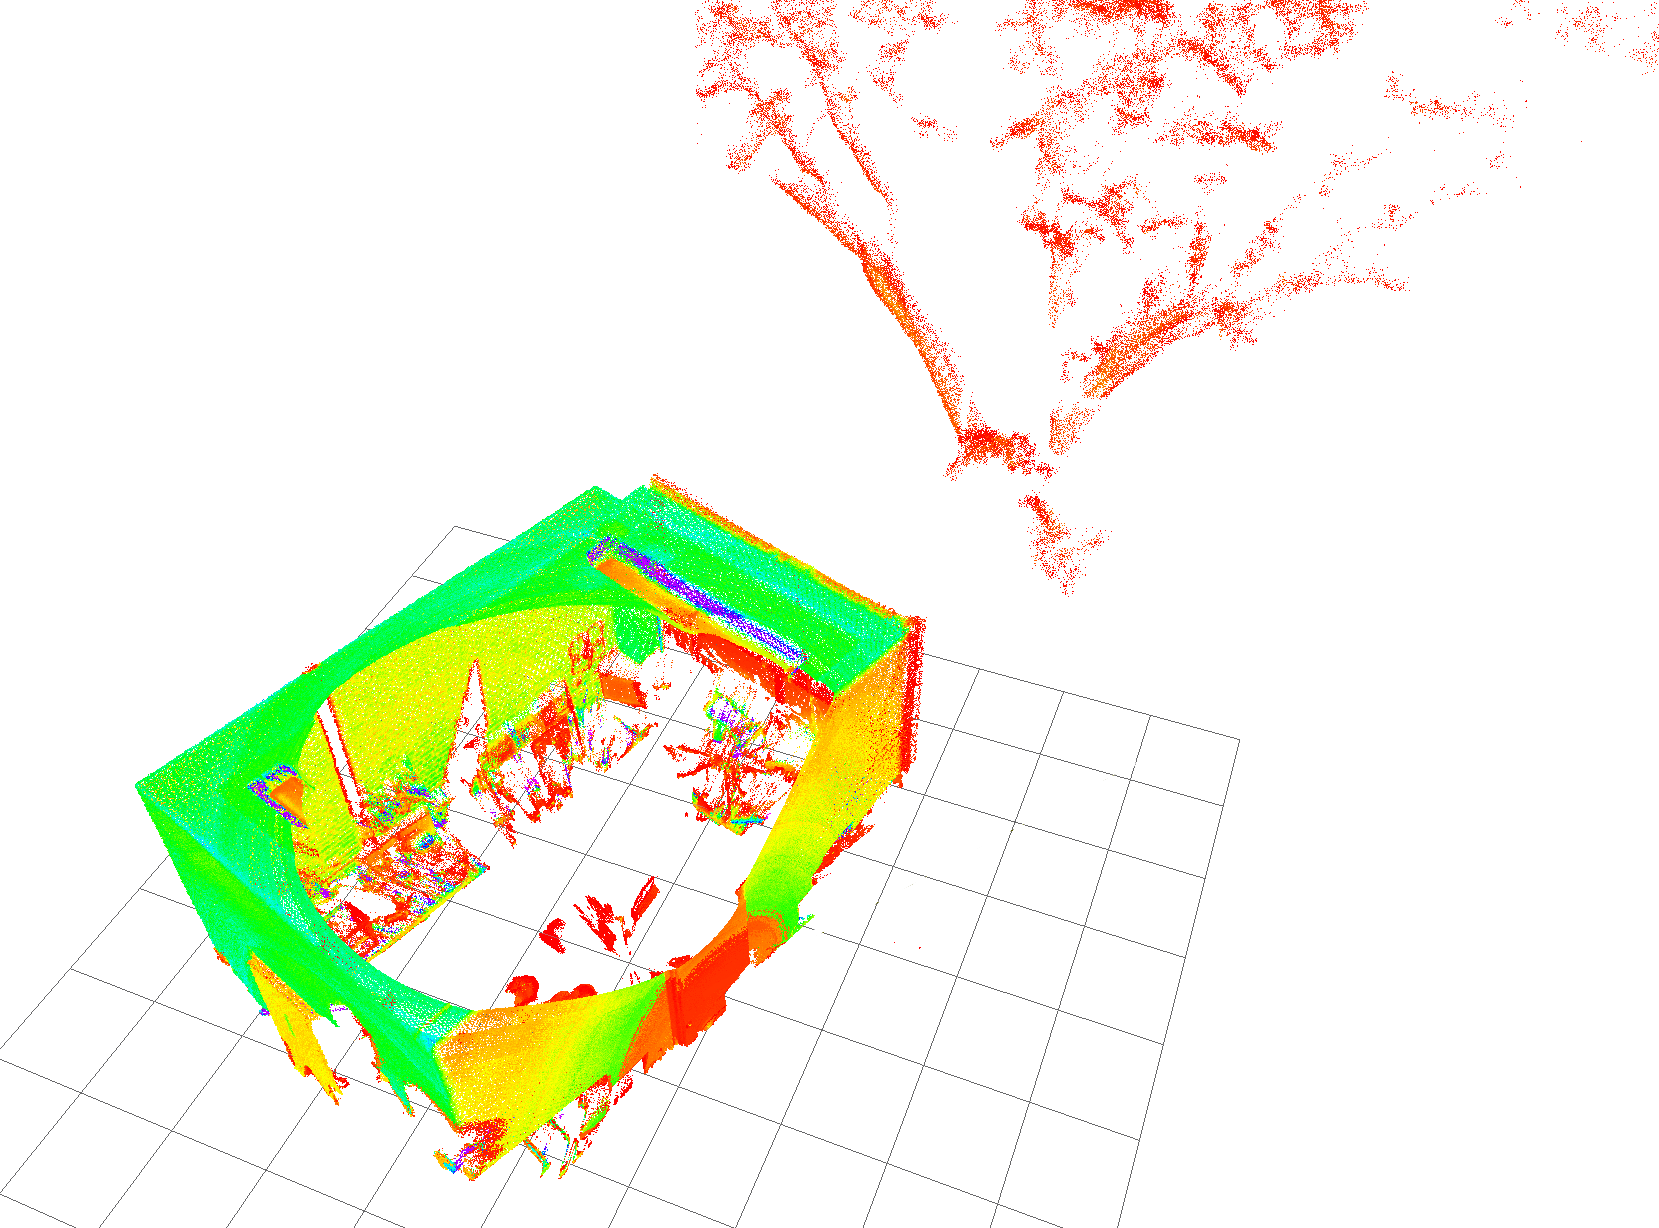
\includegraphics[width=0.7\textwidth]{Images/ldiar_scan_deadzone.png}
            \caption{Blind spots in the ceiling and the floor, in a real static LIDAR scan}
            \label{fig:real_lidar_scan}
        \end{figure}

        \subsubsection{IMU}

        Gazebo has a built-in IMU sensor that can be added to the robot's description, which our mapping algorithm needs for point cloud deskewing and alignment as discussed in \ref{section:lidar_inertial_odometry}. The IMU sensor can be configured to have a certain update rate, noise, and bias. Noise can be added to the IMU sensor to simulate the noise in the IMU data. An example of an IMU sensor configuration can be seen in listing \ref{lst:imu_sensor}.

    \vspace{10pt }
\begin{minipage}{0.9\textwidth}
\begin{lstlisting}[style=xmlStyle, caption={IMU Sensor Configuration}, label={lst:imu_sensor}]
<gravity>true</gravity>
<sensor name="imu_sensor" type="imu">
    <always_on>true</always_on>
    <update_rate>100</update_rate>
    <visualize>true</visualize>
    <topic>default_topic</topic>
    <plugin filename="libgazebo_ros_imu_sensor.so" name="imu_plugin">
    <topicName>imu</topicName>
    <bodyName>imu</bodyName>
    <updateRateHZ>100.0</updateRateHZ>
    <xyzOffset>0 0 0</xyzOffset>
    <rpyOffset>0 0 0</rpyOffset>
    <frameName>imu</frameName>
    <initial_orientation_as_reference>false</initial_orientation_as_reference>
    <noise>
        <type>gaussian</type>
        <rate>
            <x>0.01</x>
            <y>0.01</y>
            <z>0.01</z>
        </rate>
        <acceleration>
            <x>0.01</x>
            <y>0.01</y>
            <z>0.01</z>
        </acceleration>
    </noise>
    </plugin>
</sensor>
\end{lstlisting}
\end{minipage}

        \subsubsection{Camera}

        In gazebo, cameras can be simulated by modifying the robot's description and adding a sensor tag to the robot's description. The camera sensor can be configured to have a certain field of view, resolution, and clipping planes. The camera sensor can also be configured to always be on, to have a certain update rate, to visualize the image, and to publish the image to a certain topic. An example of a camera sensor configuration can be seen in listing \ref{lst:camera_sensor}.

\vspace{10pt }
\begin{minipage}{0.9\textwidth}
\begin{lstlisting}[style=xmlStyle, caption={Camera Sensor Configuration}, label={lst:camera_sensor}]
<sensor name="camera" type="camera">
    <camera>
        <horizontal_fov>1.047</horizontal_fov>
        <image>
            <width>320</width>
            <height>240</height>
        </image>
    </camera>
    <always_on>1</always_on>
    <update_rate>30</update_rate>
    <visualize>true</visualize>
    <topic>camera</topic>
</sensor>
\end{lstlisting}
\end{minipage}



        Similarly, a depth camera can be simulated, as we intend to add am Intel RealSense D435 to the quadruped platform. The depth camera can be configured to have a certain field of view, resolution, clipping planes, and update rate. As depth camera tend to be noisy in the depth data, the noise can be added to the depth data. An example of a depth camera sensor configuration can be seen in listing \ref{lst:depth_camera_sensor}. Here, the noise is set to be Gaussian with a mean of 0.0 and a standard deviation of 0.01. Those values were not measured but are a good starting point for the simulation. In the case of the depth camera, the clipping planes are set to 0.05 and 8.0 meters, as the depth camera is not able to see further than 8 meters. The depth camera is also configured to have a reduced resolution of just 640x480 pixels. Both color and depth views can be seen in Figure \ref{fig:cameras_simulation_view}.
        
\vspace{10pt }
\begin{minipage}{0.9\textwidth}      
\begin{lstlisting}[style=xmlStyle, caption={Depth Camera Sensor Configuration}, label={lst:depth_camera_sensor}]
<sensor name="camera" type="depth">
    <visualize>true</visualize>
    <update_rate>10</update_rate>
    <camera>
        <horizontal_fov>1.089</horizontal_fov>
        <image>
            <format>R8G8B8</format>
            <width>640</width>
            <height>480</height>
        </image>
        <clip>
            <near>0.05</near>
            <far>8.0</far>
        </clip>
    </camera>
    <plugin name="camera_controller" 
    filename="libgazebo_ros_camera.so">
    </plugin>
</sensor>
\end{lstlisting}
\end{minipage}

\begin{figure}[H]
    \centering
    \subfigure[RGB camera view]{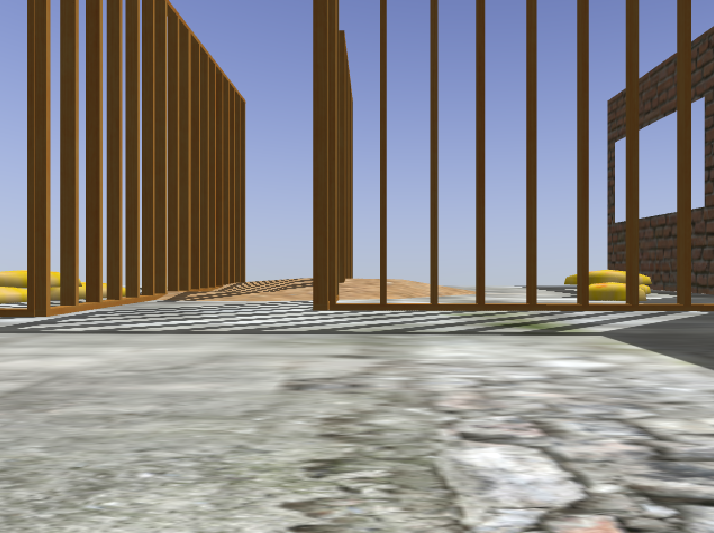
\includegraphics[width=0.45\textwidth]{Images/rviz_rgb.png}}
    \subfigure[Depth camera view]{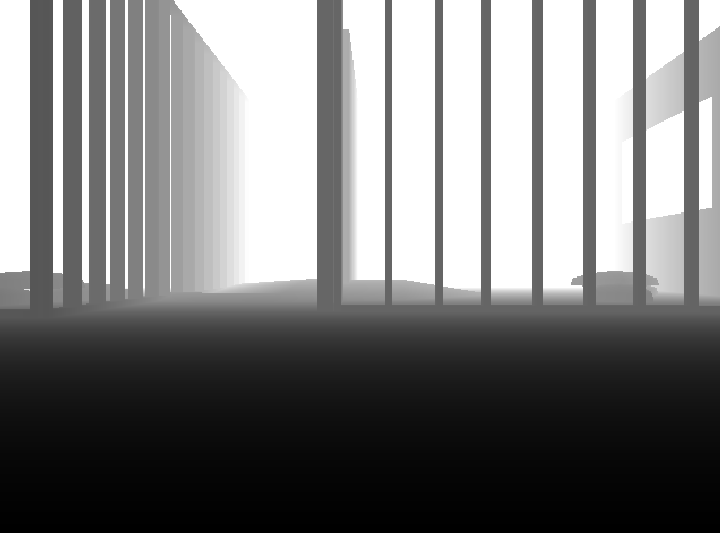
\includegraphics[width=0.45\textwidth]{Images/rviz_depth.png}}
    \caption{RGB and depth camera simulation view}
    \label{fig:cameras_simulation_view}
\end{figure}

    \subsubsection{Simulated world}

    As the target application of this multi agent exploration is to map a construction environment, a simulated world of an office in construction was created. The world is mainly based on the Gazebo office world by Clearpath Robotics and has two versions : one in construction with walls being built and construction equipment all over, and one where the office is constructed as can be seen in figure \ref{fig:office_world}. The figure also shows the acquired pint cloud from a stationary LIDAR in the office world. 

    \begin{figure}[H]
        \centering
        \subfigure[Office in construction point-cloud]{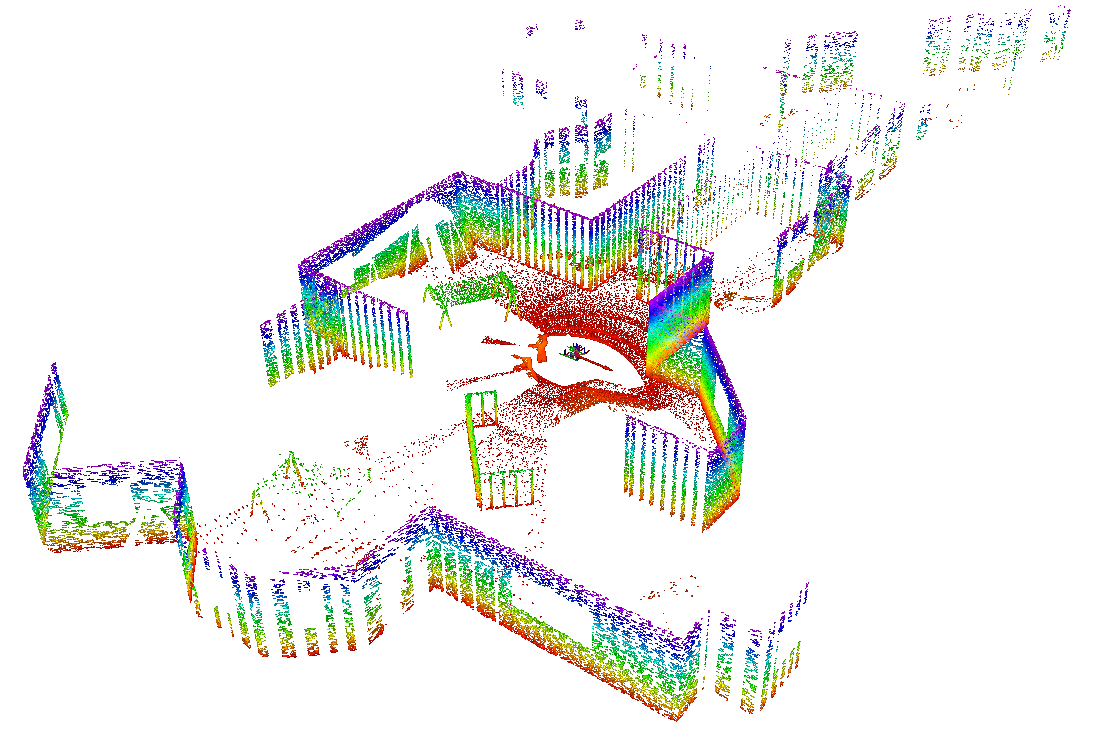
\includegraphics[width=0.49\textwidth]{Images/construction rviz.png}}
        \subfigure[Office constructed point-cloud]{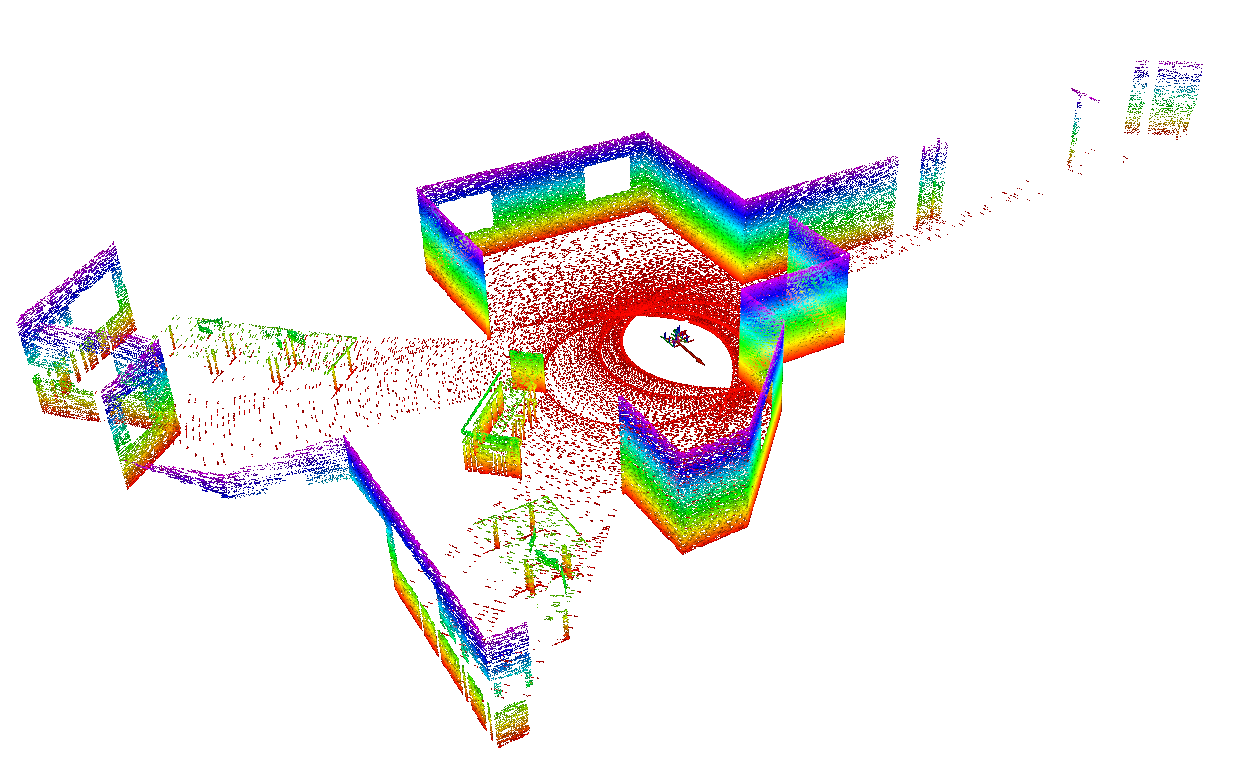
\includegraphics[width=0.49\textwidth]{Images/office_constructed_rviz.png}}
        \subfigure[Office in construction gazebo]{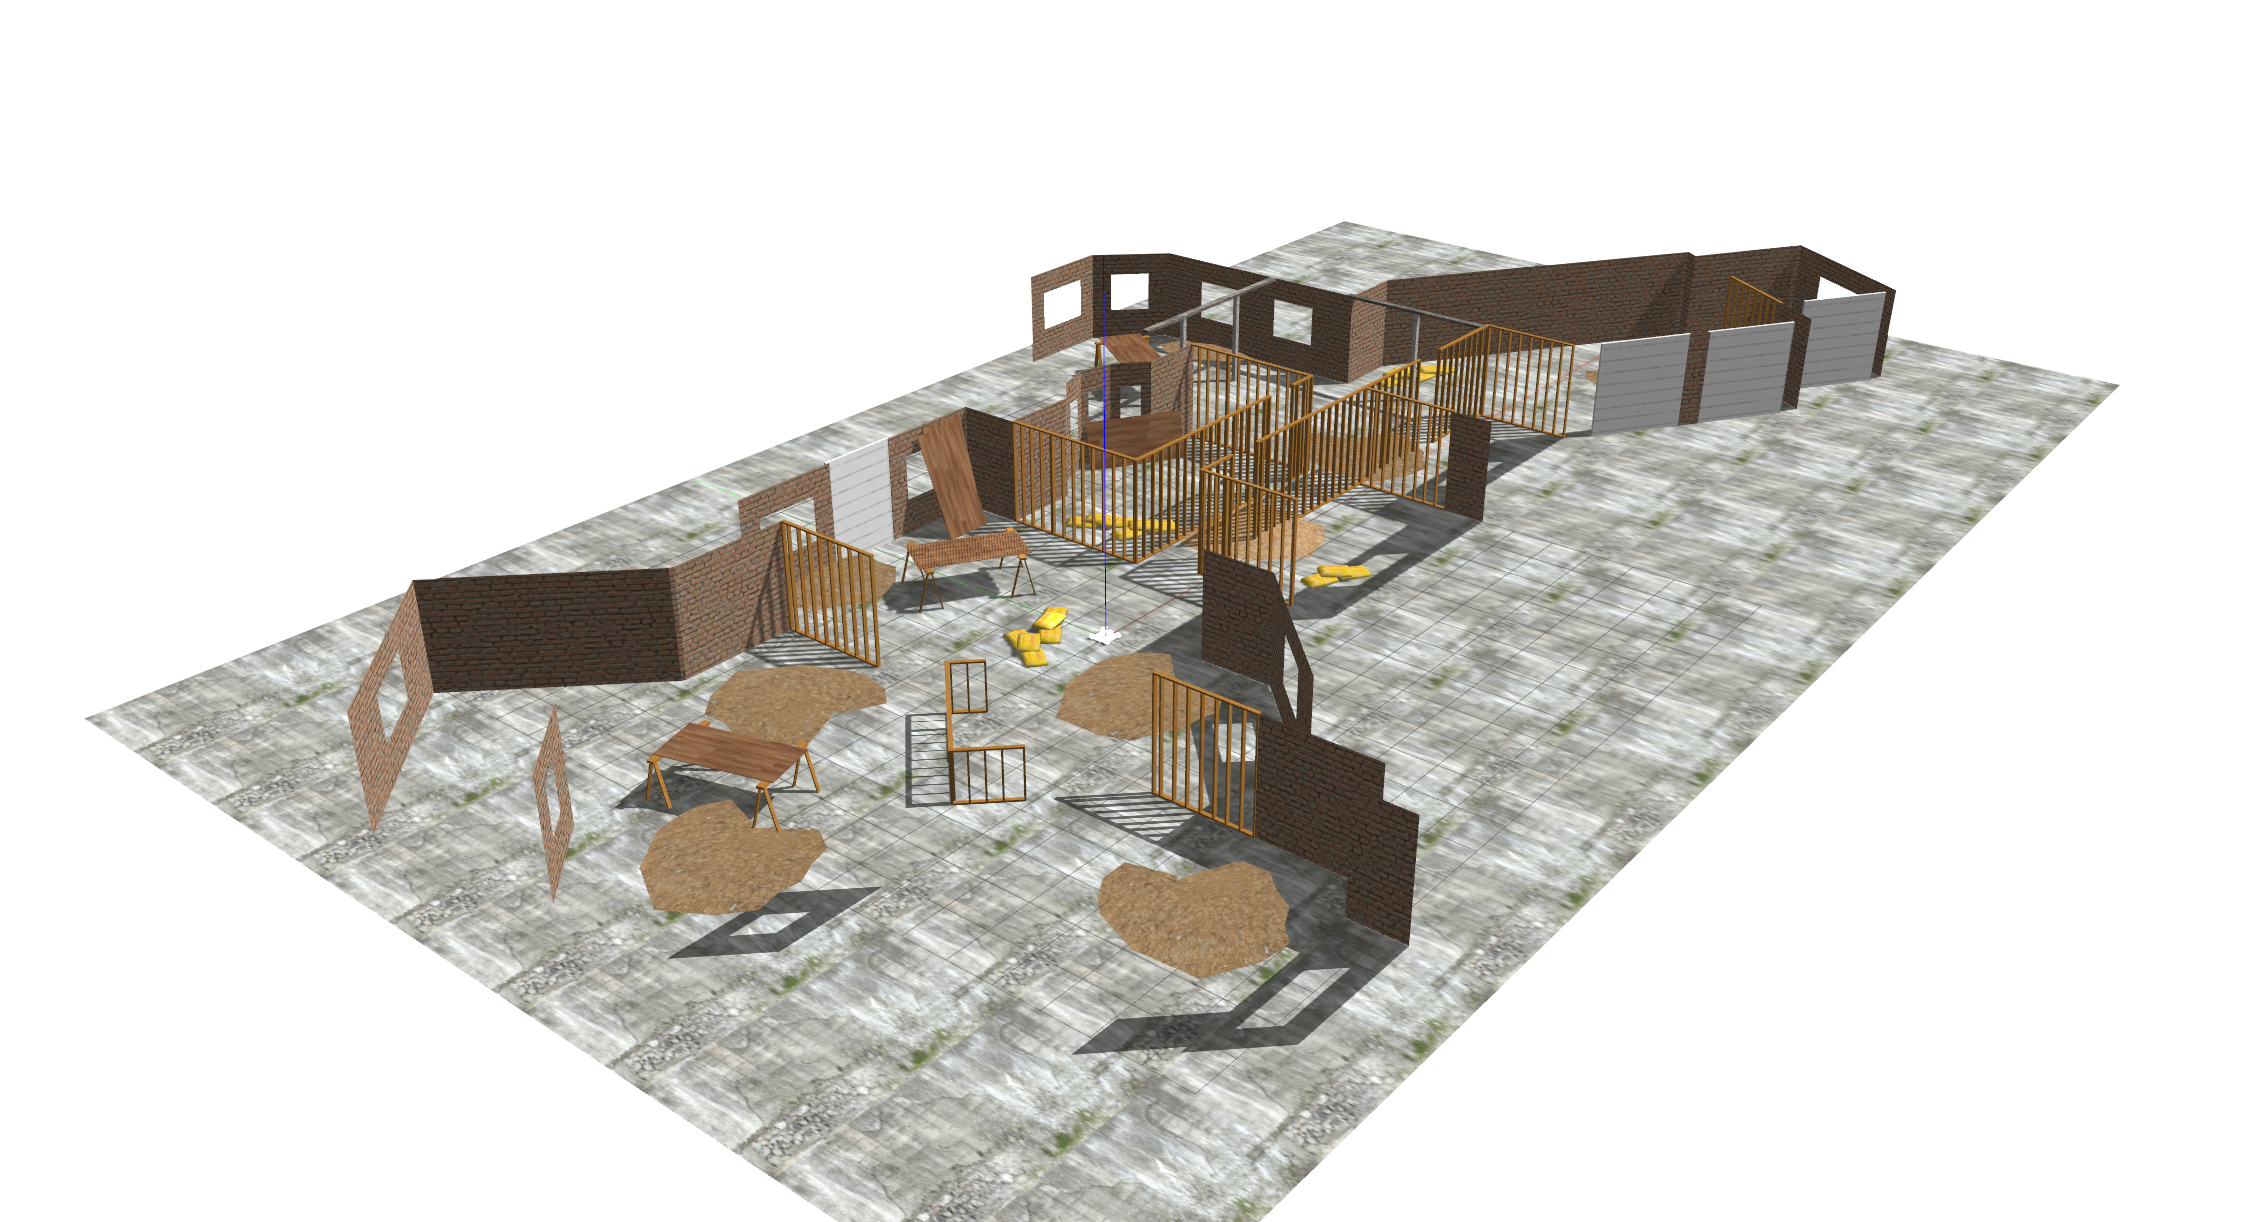
\includegraphics[width=0.49\textwidth]{Images/Construction_gazebo.png}}
        \subfigure[Office constructed]{\includegraphics[width=0.49\textwidth]{Images/office_constructed_gazebo.png}}
        \caption{Office world in construction and constructed}
        \label{fig:office_world}
    \end{figure}

    To test the planning algorithms, a more complex environment with more ramps, stairs, and difference in level would have been interesting to develop. However, a lack of time meant that the simulation remained simple, opting for prebuilt environment like the one developped for the Falco paper \cite{zhang2020falco}. They provide 5 environments like a multi-level parking garage, a university campus, a tunnel network, onw with indoor corridors, and a forest. 
    
    \begin{figure}[H]
        \centering
        \includegraphics[width=0.8\textwidth]{Images/falco_environments.png}
        \caption{Environments used in the Falco paper}
        \label{fig:falco_environments}
    \end{figure}
    
    These environments (Figure \ref{fig:falco_environments}), offer different settings like narrow passages, dead-ends, or large areas to explore. They were subsequently used to test the exploration algorithms like TARE and MTARE.

\section{Contributions}

    With this internship, I bring a low-cost exploration platform that can autonomously map and explore unknown environments. The quadruped platform is especially interesting as it uses a dedicated LIDAR for navigation, exploration, and planning, and a second LIDAR for mapping. This relives some effort from the embedded computer that can perform most of the decisions using a low point per second LIDAR, while the second LIDAR requires a very low amount of processing for mapping. Furthermore, the quadruped platform can be used to explore areas that are difficult to reach for wheeled platforms, like stairs, ramps, or uneven terrain. Stairs remain difficult for a platform of this size, but other platform like Boston Dynamics' Spot, Anybotics' Anymal, or Unitree B2 and B2W have shown tremendous capabilities in this area.

    Additionally, during this internship several contributions to open source projects were made. Following is a list of commits and pull request made to open source projects during this internship :

    % gazebosim/gz-gui | pr | Added dark mode for drawer and menu buttons | merged
    % gazebosim/docs | pr |Update ros_installation.md as Jazzy is now released | merged
    % gazebosim/gz-msgs | issue | MessageFactory::Types returns duplicate message types | opened and fixed
    % gazebo-web/gzweb | pr | Add missing primitive model support | merged
    % ros2/ros2_documentation | pr | Changed the description of the clang compile setup | merged
    % ros-navigation/nav2 | pr | precomputeDistanceHeuristic is now computed once | merged
    % ros-control/gz_ros_control | pr | Changed command for gui launch to gz instead of ign | merged 
    % FreeCAD/FreeCAD | issue | Start: Thumbnail is not displayed if name of file contains dot | open
    % FreeCAD/FreeCAD | pr | Gui: allow LineEdit to grow with text - fixes #17747
    % FreeCAD/FreeCAD | code review | Assembly: prescribed motions
    \begin{table}[H]
        \centering
        \small
        \mbox{}\clap{
        \begin{tabular}{|l|l|l|l|}
            \hline
            \textbf{Repository} & \textbf{Type} & \textbf{Description} & \textbf{Status} \\ \hline
            gazebosim/gz-gui & pr & Added dark mode for drawer and menu buttons & merged \\ \hline
            gazebosim/docs & pr & Update ros\_installation.md as Jazzy is now released & merged \\ \hline
            gazebosim/gz-msgs & issue & MessageFactory::Types returns duplicate message types & open\\ \hline
            gazebo-web/gzweb & pr & Add missing primitive model support & merged \\ \hline
            ros2/ros2\_documentation & pr & Changed the description of the clang compile setup & merged \\ \hline
            ros-navigation/nav2 & pr & precomputeDistanceHeuristic is now computed once & merged \\ \hline
            ros-control/gz\_ros\_control & pr & Changed command for gui launch to gz instead of ign & merged \\ \hline
            FreeCAD/FreeCAD & issue & Start: Thumbnail is not displayed if name of file contains dot & open \\ \hline
            FreeCAD/FreeCAD & pr & Gui: allow LineEdit to grow with text - fixes \#17747 & open \\ \hline
            FreeCAD/FreeCAD & code review & Assembly: prescribed motions & open \\ \hline
        \end{tabular}
        }
        \caption{Contributions to open source projects}
        \label{tab:contributions}
    \end{table}

    The reverse engineering efforts of the GO2 battery and the internal firmware that were documented in section \ref{section:go2_battery} were also shared with the community. These efforts aim to help in the development of an open source firmware for the GO2.

    The work on making the TARE planner work with the Unitree GO2 will also help accelerate the development of exploration algorithms for the quadruped platform, with our solution being a low cost and open source alternative to other solutions based on expensive hardware and proprietary software. The configuration we used for the TARE planner with the GO2 can be found in Listing \ref{lst:tare_config}.

    % TODO : add in annex working configuration of TARE for a GO2


\newpage
\section{Conclusion}
%\addcontentsline{toc}{section}{Conclusion}

    % TODO : Write the conclusion
    Conclusion     

\newpage
\bibliography{refs} % Entries are in the refs.bib file
\addcontentsline{toc}{section}{Bibliography}

\newpage
\addcontentsline{toc}{section}{Glossaire}
\printnoidxglossaries %glossaire, dans le fichier lexique.tex

\newpage
\addcontentsline{toc}{section}{List of figures}
\listoffigures


\newpage
\section*{Annexe}
\addcontentsline{toc}{section}{Annexe}
% Uncomment input annexe when needed
\begin{lstlisting}[style=yaml, caption={TARE planner parameter configuration for Unitree GO2}, label={lst:tare_config}]
tare_planner_node:
  ros__parameters:
    sub_start_exploration_topic_ : /start_exploration
    sub_terrain_map_topic_ : /terrain_map
    sub_terrain_map_ext_topic_ : /terrain_map_ext
    sub_state_estimation_topic_ : /state_estimation_at_scan
    sub_registered_scan_topic_ : /registered_scan
    sub_coverage_boundary_topic_ : /sensor_coverage_planner/coverage_boundary
    sub_viewpoint_boundary_topic_ : /navigation_boundary
    sub_nogo_boundary_topic_ : /sensor_coverage_planner/nogo_boundary
    sub_joystick_topic_ : /joy
    sub_reset_waypoint_topic_ : /reset_waypoint
    pub_exploration_finish_topic_ : exploration_finish
    pub_runtime_breakdown_topic_ : runtime_breakdown
    pub_runtime_topic_ : /runtime
    pub_waypoint_topic_ : /way_point
    pub_momentum_activation_count_topic_ : momentum_activation_count

    kAutoStart : true
    kRushHome : true
    kUseTerrainHeight : true
    kCheckTerrainCollision : true
    kExtendWayPoint : false
    kUseLineOfSightLookAheadPoint : false
    kNoExplorationReturnHome : false
    kExtendWayPointDistanceBig : 1.0
    kExtendWayPointDistanceSmall : 0.5  
    kKeyposeCloudDwzFilterLeafSize : 0.2
    kRushHomeDist : 0.05 # 5.0
    kAtHomeDistThreshold : 0.75 # 0.5
    kTerrainCollisionThreshold : 0.5
    kLookAheadDistance : 8.0
    kUseMomentum : false 
    kDirectionChangeCounterThr : 6
    kDirectionNoChangeCounterThr : 5
    kResetWaypointJoystickAxesID : 2

    # PlanningEnv
    kUseFrontier : true
    kFrontierClusterTolerance : 2.0 # 1.0
    kFrontierClusterMinSize : 5 #10
    kUseCoverageBoundaryOnFrontier : false
    kUseCoverageBoundaryOnObjectSurface : false

    # Rolling occupancy grid
    rolling_occupancy_grid/resolution_x : 0.2
    rolling_occupancy_grid/resolution_y : 0.2
    rolling_occupancy_grid/resolution_z : 0.2

    kSurfaceCloudDwzLeafSize : 0.3 # 0.3
    kCollisionCloudDwzLeafSize : 0.2 # 0.2
    kKeyposeCloudStackNum : 5 # 5
    kPointCloudRowNum : 20 # 50
    kPointCloudColNum : 20 # 50
    kPointCloudLevelNum : 30
    kMaxCellPointNum : 100000 # 100000
    kPointCloudCellSize : 5.0 # 18.0
    kPointCloudCellHeight : 1.8 # 1.8
    kPointCloudManagerNeighborCellNum : 5 # 5
    kCoverCloudZSqueezeRatio : 2.0 # 2.0

    # KeyposeGraph
    keypose_graph/kAddNodeMinDist : 1.0
    keypose_graph/kAddNonKeyposeNodeMinDist : 0.5
    keypose_graph/kAddEdgeConnectDistThr : 3.0
    keypose_graph/kAddEdgeToLastKeyposeDistThr : 3.0
    keypose_graph/kAddEdgeVerticalThreshold : 1.0
    keypose_graph/kAddEdgeCollisionCheckResolution : 0.4
    keypose_graph/kAddEdgeCollisionCheckRadius : 0.4
    keypose_graph/kAddEdgeCollisionCheckPointNumThr : 1

    # ViewPointManager
    viewpoint_manager/number_x : 30 # 50
    viewpoint_manager/number_y : 30 # 50
    viewpoint_manager/number_z : 1
    viewpoint_manager/resolution_x : 0.2 # 0.4
    viewpoint_manager/resolution_y : 0.2 # 0.4
    viewpoint_manager/resolution_z : 0.0
    kConnectivityHeightDiffThr : 0.25
    kGreedyViewPointSampleRange : 3 # 3
    kLocalPathOptimizationItrMax : 10 # 10
    kViewPointCollisionMargin : 0.25  # 0.6
    kViewPointCollisionMarginZPlus : 0.5
    kViewPointCollisionMarginZMinus : 0.5
    kCollisionGridZScale : 1.0
    kCollisionGridResolutionX : 0.2
    kCollisionGridResolutionY : 0.2
    kCollisionGridResolutionZ : 0.0
    kCollisionPointThr : 1
    kLineOfSightStopAtNearestObstacle : true
    kViewPointHeightFromTerrain : 0.3  # 0.75
    kViewPointHeightFromTerrainChangeThreshold : 0.2  # 0.6
    kCheckDynamicObstacleCollision : false
    kCollisionFrameCountMax : 3

    kSensorRange : 8.5  # 3.5
    kNeighborRange : 1.5 # 3.0
    kCoverageOcclusionThr : 0.1
    kCoverageDilationRadius : 0.9

    # Grid World
    kGridWorldXNum : 50 # 121
    kGridWorldYNum : 50 # 121
    kGridWorldZNum : 50 # 121
    kGridWorldCellHeight : 3.0 # 3.0
    kGridWorldNearbyGridNum : 5 # 5
    kMinAddPointNumSmall : 1 # 30
    kMinAddPointNumBig : 1 #60
    kMinAddFrontierPointNum : 1 #20
    kCellExploringToCoveredThr : 1
    kCellCoveredToExploringThr: 10 # 10
    kCellExploringToAlmostCoveredThr: 10 # 10
    kCellAlmostCoveredToExploringThr: 20 # 20
    kCellUnknownToExploringThr: 1

    # Visualization (parameters not working I think)
    kExploringSubspaceMarkerColorGradientAlpha : true
    kExploringSubspaceMarkerColorMaxAlpha : 0.8
    kExploringSubspaceMarkerColorR : 0.0
    kExploringSubspaceMarkerColorG : 1.0
    kExploringSubspaceMarkerColorB : 0.0
    kExploringSubspaceMarkerColorA : 1.0
    kLocalPlanningHorizonMarkerColorR : 0.0
    kLocalPlanningHorizonMarkerColorG : 1.0
    kLocalPlanningHorizonMarkerColorB : 0.0
    kLocalPlanningHorizonMarkerColorA : 1.0
    kLocalPlanningHorizonMarkerWidth : 0.05
    kLocalPlanningHorizonHeight : 3.0

\end{lstlisting}



    
\end{document}